%% monografia.tex, fabiokepler, jeancheiran
%% Copyright 2012-2018 by UNIPAMPA LaTeX group at https://bitbucket.org/unipampaalegrete/monografias-cc-es-repo/
%%
%% This work may be distributed and/or modified under the conditions of the LaTeX Project Public
%% License, either version 1.3 of this license or (at your option) any later version.
%% The latest version of this license is in
%%   http://www.latex-project.org/lppl.txt
%% and version 1.3 or later is part of all distributions of LaTeX version 2005/12/01 or later.
%%
%% Based on the example file abtex2-modelo-trabalho-academico.tex of the abntex2 package
%% (http://abntex2.googlecode.com/) and on the ppgccufmg 1.45beta2 class
%% (http://vilarneto.com/ppgccufmg,
%% http://www.dcc.ufmg.br/pos/alunos/modelodisstese.php
%% and http://www.dcc.ufmg.br/~mirella).
%%
%% Adapted for the Computer Science program at UNIPAMPA (http://www.unipampa.edu.br)
%% by Fabio Kepler (fabio@kepler.pro.br) and Jean Cheiran (jeancheiran@unipampa.edu.br).
%%
%% Version 2.5 - 2018/08
%% Version 2.4 - 2017/05
%% Version 2.3 - 2013/03

% +++++++++++++++++++++++++++++++++++++++++++++++++++++++++++++++++++++++++++++++++++++++++++++++++
% Este modelo utiliza o pacote abnTeX2. Veja como instalá-lo em seu ambiente em
% http://abntex2.googlecode.com/.
% -------------------------------------------------------------------------------------------------
% abnTeX2: Modelo de Trabalho Acadêmico (tese de doutorado, dissertação de
% mestrado e trabalhos monográficos em geral) em conformidade com
% ABNT NBR 14724:2011: Informação e documentação - Trabalhos acadêmicos -
% Apresentação
% -------------------------------------------------------------------------------------------------
% Normas institucionais utilizadas:
% http://porteiras.r.unipampa.edu.br/portais/sisbi/programa-de-capacitacao/
% +++++++++++++++++++++++++++++++++++++++++++++++++++++++++++++++++++++++++++++++++++++++++++++++++

\documentclass[12pt,openright,twoside,a4paper,chapter=TITLE,english]{abntex2}    % frente e verso
%\documentclass[12pt,oneside,a4paper]{abntex2}            % apenas frente

% +++++++++++++++++++++++++++++++++++++++++++++++++++++++++++++++++++++++++++++++++++++++++++++++++
% PACOTES
% -------------------------------------------------------------------------------------------------
% Pacotes fundamentais
\usepackage[style=abnt,backref=true]{biblatex}
\usepackage{cmap}           % Mapeamento de caracteres especiais no PDF
\usepackage{lmodern}        % Usa fonte Latin Modern
\usepackage[T1]{fontenc}    % Seleção de codificação de fonte
\usepackage[utf8]{inputenc} % Codificação do arquivo (conversão automática dos acentos)
\usepackage[brazil]{babel}  % Idioma para hifenização e tradução de vários elementos
\usepackage{makeidx}        % Criação de índice
\usepackage{hyperref}       % Formatação do índice
\usepackage{lastpage}       % Usado pela Ficha catalográfica
\usepackage{indentfirst}    % Indenta o primeiro parágrafo de cada seção
\usepackage[table,xcdraw,usenames,dvipsnames]{xcolor}  % Controle das cores (com nomes) e formatação de tabelas
\usepackage{graphicx}       % Inclusão de gráficos
\usepackage{forest}
\usepackage{booktabs}       % Formatação de tabelas
\usepackage{adjustbox}

% \usepackage{rotating}
\usepackage{lscape}

% -------------------------------------------------------------------------------------------------
% Para citações
% \usepackage[brazilian,hyperpageref]{backref} % Páginas com as citações na bibliografia
% \usepackage[alf,abnt-emphasize=bf]{abntex2cite} % Citações padrão ABNT (alfanumérico)

% -------------------------------------------------------------------------------------------------
% Pacotes opcionais
\usepackage{nomencl}        % Para criar uma lista de símbolos
\usepackage{acro}           % Para usar acrônimos e abreviaturas
\usepackage{tikz}           % Para fazer figuras, diagramas e gráficos integrados e elegantes
\usepackage{pgfplots}       % Usa o pacote tikz para fazer gráficos muito melhores que os do Excel
% \usepackage{pgfplotstable}  % Para gerar tabelas automaticamente a partir de arquivos com dados
\usepackage{filecontents}   % Para colocar o conteúdo de um arquivo dentro de um arquivo tex
\usepackage{todonotes}      % Para criar anotações durante o desenvolvimento do texto
\usepackage{multirow}       % Permite fazer tabelas com múltiplas linhas
%\let\newfloat=\undefined    % Workaround para usar o pacote algorithm
%\usepackage{algorithm}      % Para escrever algoritmos
%\usepackage{clrscode}       % Para escrever algoritmos
%\usepackage{clrscode3e}     % Para escrever algoritmos; mais simples que os pacotes acima
\usepackage{pdfpages}        % Para incluir a folha de aprovação assinada em PDF
\usepackage[olditem]{paralist}  % Listas in-line
\usepackage{colortbl}        % Cronograma (Tabelas)
\usepackage[autostyle]{csquotes} % Citações
\usepackage{url}
\usepackage{hhline}
\usepackage[nameinlink]{cleveref}
\usepackage{makecell}
\usepackage{rotating}

% \usepackage{enumerate}
\usepackage{enumitem}

\usetikzlibrary{patterns}

\usepackage{smartdiagram}

\usepackage{amssymb}

\usepackage{pgf-pie}

\smartdiagramset{circular distance=3.5cm, font=\medium, text width=2.0cm,
module minimum width=1.5cm, module minimum height=1.0cm,arrow tip=to,uniform connection color=true,uniform color list=blue!30 for 7 items}

\def\BibTeX{{\rm B\kern-.05em{\sc i\kern-.025em b}\kern-.08em
    T\kern-.1667em\lower.7ex\hbox{E}\kern-.125emX}}

%PGPLOTS
\usepackage{pgfplots}
\usetikzlibrary{patterns}
\usepgfplotslibrary[statistics] % ConTEXt
\usetikzlibrary{pgfplots.statistics} % LATEX and plain TEX
\usepackage{tikz}
\usepackage{ragged2e}

\usetikzlibrary{patterns}
%\rowcolors{1}{gray!10}{}

\usetikzlibrary{angles,shadows,positioning,backgrounds,mindmap}

\pgfplotsset{width=9cm, height=8cm, compat=1.9}

\usetikzlibrary{shapes,backgrounds}
\def\BibTeX{{\rm B\kern-.05em{\sc i\kern-.025em b}\kern-.08em
    T\kern-.1667em\lower.7ex\hbox{E}\kern-.125emX}}

% começo da bagunça
\usetikzlibrary{angles,shadows.blur,positioning,backgrounds}
\usepackage{forest}
\forestset{
  declare count register=disjuncts from,
  disjuncts from'=0,
  declare count register=concrete from,
  concrete from'=2,
  concrete colour/.code={\colorlet{concretecol}{#1}},
  abstract colour/.code={\colorlet{abstractcol}{#1}},
  draw colour/.code={\colorlet{drawcol}{#1}},
  concrete colour=gray,
  abstract colour=white,
  draw colour=black,
  /tikz/mandatory/.style={circle, fill=drawcol, draw=drawcol},
  /tikz/optional/.style={circle, draw=drawcol, fill=white},
  /tikz/concrete/.style={fill=concretecol, draw=drawcol},
  /tikz/abstract/.style={fill=abstractcol, draw=drawcol},
  /tikz/or/.style={},
  mandatory/.style={edge label={node [mandatory] {}}},
  optional/.style={edge label={node [optional] {}}},
  or/.style={for first={disjunct}},
  disjunct/.style={
    tikz+={\path (.parent) coordinate (A) -- (!u.children) coordinate (B) -- (!ul.parent) coordinate (C) pic [fill=drawcol] {angle};}
  },
  disjunction tree/.style={
    where={isodd(n_children())}{
      for n={int((n_children()+1)/2)}{calign with current},
    }{
      calign=midpoint,
    },
    before typesetting nodes={
      for nodewalk={
        filter/.wrap pgfmath arg={{level>=##1}{n_children()>1}}{(disjuncts_from)}
      }{
        or,
      },
      where={level()>=(concrete_from)}{
        concrete,
      }{
        abstract,
      },
      tikz+={
        [font=\sffamily]
        \node (l) [anchor=north east, xshift=10pt] at (current bounding box.north east) {Legend};
        \foreach \i/\j [remember=\i as \k (initially l)] in {mandatory/Mandatory,optional/Optional,or/Or,abstract/Abstract,concrete/Concrete}
        {
          \node (\i) [below=20pt of \k.north, anchor=north, text centered, \i, minimum width=5pt,] {};
          \node (\j) [right=15pt of \i.center -| mandatory.west, anchor=west] {\j};
        };
        \draw [drawcol] (or.south west) coordinate (A) -- (or.north) coordinate (B) -- (or.south east) coordinate (C) pic [fill=drawcol, angle radius=5pt] {angle};
        \foreach \i in {mandatory,optional} \draw [darkgray] (\i.north east) -- +(45:5pt);
        \node (c) [below=0pt of Concrete.south] {};
        \scoped[on background layer]{\node [draw, fill=white, blur shadow, fit=(l) (Mandatory) (Optional) (Or) (Abstract) (Concrete) (c), rounded corners] {};}
      },
    },
    for tree={
      parent anchor=children,
      child anchor=parent,
      l'+=10mm,
      blur shadow,
      rounded corners,
      text height=2ex,
      text depth=.5ex,
      font=\sffamily,
    }
    % qtree/.style={
    %     for tree={
    %         parent anchor=south, 
    %         child anchor=north,
    %         align=center,
    %         inner sep=0pt,
    %         l'+=10mm,
    %         blur shadow,
    %         rounded corners,
    %         text height=2ex,
    %         text depth=.5ex,
    %         font=\sffamily,
    %     }
    % },
  },
}

% -------------------------------------------------------------------------------------------------
% Configurações de pacotes
% -------------------------------------------------------------------------------------------------

\addto\captionsenglish{% ingles
  %% adjusts names from abnTeX2
  \renewcommand{\folhaderostoname}{Title page}
  \renewcommand{\epigraphname}{Epigraph}
  \renewcommand{\dedicatorianame}{Dedication}
  \renewcommand{\errataname}{Errata sheet}
  \renewcommand{\agradecimentosname}{Acknowledgements}
  \renewcommand{\anexoname}{ANNEX}
  \renewcommand{\anexosname}{Annex}
  \renewcommand{\apendicename}{APPENDIX}
  \renewcommand{\apendicesname}{Appendix}
  \renewcommand{\orientadorname}{Supervisor:}
  \renewcommand{\coorientadorname}{Co-supervisor:}
  \renewcommand{\folhadeaprovacaoname}{Approval}
  \renewcommand{\resumoname}{Resumo} 
  \renewcommand{\listadesiglasname}{List of Abbreviations and acronyms}
  \renewcommand{\listadesimbolosname}{List of Symbols}
  \renewcommand{\fontename}{Source}
  \renewcommand{\notaname}{Note}
   %% adjusts names used by \autoref
  \renewcommand{\pageautorefname}{page}
  \renewcommand{\chapterautorefname}{Chapter}
  \renewcommand{\figureautorefname}{Figure}
  \renewcommand{\tableautorefname}{Table}
  \renewcommand{\sectionautorefname}{Section}
  \renewcommand{\subsectionautorefname}{Section}
  \renewcommand{\subsubsectionautorefname}{Section}
  \renewcommand{\paragraphautorefname}{Section}
%   \renewcommand{\englishbibname}{References}
%   \renewcommand{\englishindexname}{Index}
%   \renewcommand{\englishlistfigurename}{List of Figures}
%   \renewcommand{\englishfigurename}{Figure}
%   \renewcommand{\englishlisttablename}{List of Tables}
%   \renewcommand{\englishtablename}{Table}
%   \renewcommand{\englishcontentsname}{List of Contents}
%   \renewcommand{\englishchaptername}{Chapter}
  \renewcommand{\imprimirtipotrabalho}{Term Paper }
}

% -------------------------------------------------------------------------------------------------
% Configurações do pacote backref
% Usado sem a opção hyperpageref de backref
% \renewcommand{\backrefpagesname}{Cited in page(s):~}
% \renewcommand*{\backrefsep}{,~}%
% \renewcommand*{\backreftwosep}{,~}% ', and~'
% \renewcommand*{\backreflastsep}{,~}% ' and~'
% % Texto padrão antes do número das páginas
% \renewcommand{\backref}{}
% % Define os textos da citação
% \renewcommand*{\backrefalt}[4]{
%     \ifcase #1 %
%         No text citation.%
%     \or
%         Cited in page #2.%
%     \else
%         Cited #1 times on pages #2.%
%     \fi}%
% -------------------------------------------------------------------------------------------------
% Configurações de aparência do PDF final
%\definecolor{blue}{RGB}{41,5,195}
% \definecolor{webgreen}{rgb}{0,.5,0}
% Metainformações do PDF e cores dos links
\hypersetup{
  portuguese,
  %backref=true,
  %pagebackref=true,
  %bookmarks=true,             % show bookmarks bar?
  %bookmarksnumbered=true,
  bookmarksdepth=4,
  pdftitle={\@title},
  pdfauthor={\@author},
  pdfsubject={\imprimirpreambulo},
  pdfkeywords={UNIPAMPA}{Computação}{UNIPAMPA}{abntex}{TCC},
  %pdfproducer={LaTeX with abnTeX2},     % producer of the document
  pdfcreator={\@author},
  colorlinks=true,           % false: boxed links; true: colored links
  linkcolor=black,            % color of internal links
  citecolor=black,            % color of links to bibliography
  filecolor=black,         % color of file links
  urlcolor=black
}
%   linktocpage,
%   colorlinks,
%   citecolor=webgreen,
%   urlcolor=Maroon,
%   linkcolor=RoyalBlue,
%   filecolor=black,
% -------------------------------------------------------------------------------------------------
% Espaçamentos entre linhas e parágrafos
% O tamanho do parágrafo é dado por
\setlength{\parindent}{1.3cm}
% Controle do espaçamento entre um parágrafo e outro
\setlength{\parskip}{0.2cm} % tente também \onelineskip
% Controles do espaçamento entre linhas
%\OnehalfSpacing       % espaçamento um e meio (padrão);
%\DoubleSpacing        % espaçamento duplo
%\SingleSpacing        % espaçamento simples
% -------------------------------------------------------------------------------------------------
% Para o pacote de acrônimos
\acsetup{make-links} %first-style=short}
% -------------------------------------------------------------------------------------------------
% Para o pacote tikz, pgfplots e pgfplotstable
\usetikzlibrary{arrows,chains,matrix,positioning,decorations.pathreplacing,calc}
% -------------------------------------------------------------------------------------------------
% Para poder usar subfiguras e subtabelas
\newsubfloat{figure}
\newsubfloat{table}
\providecommand*{\subfigureautorefname}{\figureautorefname}
% +++++++++++++++++++++++++++++++++++++++++++++++++++++++++++++++++++++++++++++++++++++++++++++++++


% +++++++++++++++++++++++++++++++++++++++++++++++++++++++++++++++++++++++++++++++++++++++++++++++++
% Informações de dados para CAPA e FOLHA DE ROSTO
% -------------------------------------------------------------------------------------------------
\titulo{Extensionly - A tool for supporting the management of outreach projects and programs in the university: Backend}

\autor{Igor Dalepiane da Costa}
\local{Alegrete}
\data{2022}
\orientador{Prof. PhD. Maicon Bernardino da Silveira}

% \coorientador{Prof. <titulação> Nome do Coorientador} % Se houver
\instituicao{FEDERAL UNIVERSITY OF PAMPA}
\tipotrabalho{Projeto de Trabalho de Conclusão de Curso~} % Para TCC I
% \tipotrabalho{Trabalho de Conclusão de Curso~} % Para TCC II
% O preambulo deve conter o tipo do trabalho, o objetivo, o nome da instituição e a área de concentração
\preambulo{\imprimirtipotrabalho presented in Software Engineering Graduation Course in the Federal University of Pampa as a partial requirement for obtaining the title of Software Engineering
Bachelor}
% +++++++++++++++++++++++++++++++++++++++++++++++++++++++++++++++++++++++++++++++++++++++++++++++++
\setlength\bibitemsep{1.8\itemsep}
\addbibresource{bibliografia.bib}
\makeindex % Compila o indice
\makenomenclature % Compila a lista de abreviaturas e siglas

% Abreviaturas 
\DeclareAcronym{fig}{
  short = Fig.,
  long  = Figura,
  tag = abreviaturas
}
% Acrônimos/Siglas
\DeclareAcronym{API}{
  short = API,
  long  = Application Programming Interface,
  tag = acronimos
}
\DeclareAcronym{ATE}{
  short = ATE,
  long  = Administrative Technician in Education,
  tag = acronimos
}
\DeclareAcronym{CAEX}{
  short = CAEX,
  long  = Outreach Actions Control,
  tag = acronimos
}
\DeclareAcronym{CLE}{
  short = CLE,
  long  = Local Outreach Committee,
  tag = acronimos
}
\DeclareAcronym{CONSUNI}{
  short = CONSUNI,
  long  = University Council,
  tag = acronimos
}
\DeclareAcronym{CSE}{
  short = CSE,
  long  = Superior Outreach Committee,
  tag = acronimos
}
\DeclareAcronym{DBMS}{
  short = DBMS,
  long  = Database Management System,
  tag = acronimos
}
\DeclareAcronym{FOREXT}{
  short = FOREXT,
  long  = National Forum for Outreach and Community Action of Universities and Community Higher Education Institutions,
  tag = acronimos
}
\DeclareAcronym{FORPROEX}{
  short = FORPROEX,
  long  = Forum of Pro-Rectors for Outreach of Brazilian Public Universities,
  tag = acronimos
}
\DeclareAcronym{FR}{
  short = FR,
  long  = Functional Requirement,
  tag = acronimos
}
\DeclareAcronym{HECI}{
  short = HECI,
  long  = Higher Education Community Institution,
  tag = acronimos
}
\DeclareAcronym{HEI}{
  short = HEI,
  long  = Higher Education Institution,
  tag = acronimos
}
\DeclareAcronym{HTTP}{
  short = HTTP,
  long  = Hypertext Transfer Protocol,
  tag = acronimos
}
\DeclareAcronym{ICES}{
  short = ICES,
  long  = Higher Education Community Institution,
  tag = acronimos
}
\DeclareAcronym{ID}{
  short = ID,
  long  = {Identification},
  tag = acronimos
}
\DeclareAcronym{IDP}{
  short = IDP,
  long  = Institutional Development Plan,
  tag = acronimos
}
\DeclareAcronym{JS}{
  short = JS,
  long  = JavaScript,
  tag = acronimos
}
\DeclareAcronym{MEC}{
  short = MEC,
  long  = Ministry of Education,
  tag = acronimos
}
\DeclareAcronym{MoSCoW}{
  short = MoSCoW,
  long  = {Must have, Should have, Could have and Will not have},
  tag = acronimos
}
\DeclareAcronym{MVP}{
  short = MVP,
  long  = Minimum Viable Product,
  tag = acronimos
}
\DeclareAcronym{MySQL}{
  short = MySQL,
  long  = My Structured Query Language,
  tag = acronimos
}
\DeclareAcronym{NGO}{
  short = NGO,
  long  = Non-Governmental Organization,
  long-plural-form = Non-Governmental Organizations,
  tag = acronimos
}
\DeclareAcronym{OA}{
  short = OA,
  long  = Outreach Activity,
  long-plural-form = Outreach Activities,
  tag = acronimos
}
\DeclareAcronym{ORM}{
  short = ORM,
  long  = Object Relational Mapper,
  long-plural-form = Object Relational Mappers,
  tag = acronimos
}

\DeclareAcronym{PROEXT}{
  short = PROEXT,
  long  = Dean of Outreach and Culture,
  tag = acronimos
}
\DeclareAcronym{OCA}{
  short = OCA,
  long  = Outreach Curriculum Activity,
  long-plural-form = Outreach Curriculum Activities,
  tag = acronimos
}
\DeclareAcronym{ProExt}{
  short = ProExt,
  long  = University Outreach Program,
  tag = acronimos
}
\DeclareAcronym{PR}{
  short = PR,
  long  = Pull Request,
  tag = acronimos
}
\DeclareAcronym{REST}{
  short = REST,
  long  = Representational State Transfer,
  tag = acronimos
}
\DeclareAcronym{SAP}{
  short = SAP,
  long  = Academic Project System,
  tag = acronimos
}
\DeclareAcronym{SEI}{
  short = SEI,
  long  = Electronic Information System,
  tag = acronimos
}
\DeclareAcronym{SGCE}{
  short = SGCE,
  long  = Electronic Certificate Management System,
  tag = acronimos
}
\DeclareAcronym{SIGAA}{
  short = SIGAA,
  long  = Integrated Academic Activities Management System,
  tag = acronimos
}
\DeclareAcronym{SIPPEE}{
  short = SIPPEE,
  long  = {Information System for Research, Teaching and Outreach Projects},
  tag = acronimos
}
\DeclareAcronym{TP}{
  short = TP,
  long  = Term Paper,
  long-plural-form = Term Papers,
  tag = acronimos
}
\DeclareAcronym{TS}{
  short = TS,
  long  = TypeScript,
  tag = acronimos
}
\DeclareAcronym{UNIPAMPA}{
  short = UNIPAMPA,
  long  = Federal University of Pampa,
  tag = acronimos
}
\DeclareAcronym{CD}{
  short = CD,
  long  = Continuous Deployment,
  tag = acronimos
}
\DeclareAcronym{CDE}{
  short = CDE,
  long  = Continuous Delivery,
  tag = acronimos
}
\DeclareAcronym{CI}{
  short = CI,
  long  = Continuous Integration,
  tag = acronimos
}
\DeclareAcronym{DevOps}{
  short = DevOps,
  long  = Development Operations,
  tag = acronimos
}
\DeclareAcronym{PaaS}{
  short = PaaS,
  long  = Platform as a Service,
  tag = acronimos
}





















% \DeclareAcronym{FORPROEX}{
%   short = FORPROEX,
%   long  = Forum of Pro-Rectors for Outreach of Brazilian Public Universities,
%   tag = acronimos
% }





% \DeclareUnicodeCharacter{0301}{*************************************}
% ************************************************************************************************
\begin{document}
% Pequenos consertos e ajustes para que fique de acordo com o Manual de Normatização 2011.

\setlength{\ABNTEXsignwidth}{12cm}

% ---
% Impressão da Capa
\renewcommand{\imprimircapa}{%
  \begin{capa}%
    \center
    {\ABNTEXchapterfont\large\MakeUppercase\imprimirinstituicao}

    \vspace*{\fill}
    {\ABNTEXchapterfont\large\imprimirautor}

    \vspace*{\fill}
    {\ABNTEXchapterfont\bfseries\LARGE\imprimirtitulo}

    \vspace*{\fill}
    ~
    \vspace*{\fill}

    {\large\imprimirlocal}
    \par
    {\large\imprimirdata}

    \vspace*{1cm}
  \end{capa}
}
% ---


% ---
% Impressão da Folha de Rosto
\makeatletter
\renewcommand{\folhaderostocontent}{
  \begin{center}

    {\ABNTEXchapterfont\large\imprimirautor}

    \vspace*{\fill}%\vspace*{\fill}
    {\ABNTEXchapterfont\bfseries\Large\imprimirtitulo}
    \vspace*{\fill}

    \abntex@ifnotempty{\imprimirpreambulo}{%
      \hspace{.45\textwidth}
      \begin{minipage}{.5\textwidth}
        {\SingleSpacing
        \imprimirpreambulo}

        \vspace*{1em}
        \imprimirorientadorRotulo~\imprimirorientador\par

        \abntex@ifnotempty{\imprimircoorientador}{%
          \vspace*{1em}
          \imprimircoorientadorRotulo~\imprimircoorientador%
        }%

      \end{minipage}%
      \vspace*{\fill}
    }%

    {\large\imprimirlocal}
    \par
    {\large\imprimirdata}
    \vspace*{1cm}

  \end{center}
}
\makeatother
% ---

% ---
\renewcommand{\ABNTEXchapterfont}{\rmfamily\bfseries}
\setsecheadstyle{\rmfamily\bfseries}

\renewcommand{\ABNTEXchapterfontsize}{\normalsize}
\renewcommand{\ABNTEXsectionfontsize}{\normalsize}
\renewcommand{\ABNTEXsubsectionfontsize}{\normalsize}
\renewcommand{\ABNTEXsubsubsectionfontsize}{\normalsize}
\renewcommand{\ABNTEXsubsubsubsectionfontsize}{\normalsize}

% Espaçamento entre título e texto
\setlength\afterchapskip{\lineskip}

% Espaçamento entre parágrafos
\setlength{\parskip}{0.cm}

% ---

 % Inclui alguns ajustes finos para que fique de acordo com o Manual de Normatização
\selectlanguage{english}

\imprimircapa % Capa [OBRIGATÓRIO]
\imprimirfolhaderosto % Folha de rosto [OBRIGATÓRIO]

% -----------------------------------------------
% Folha de aprovação [OBRIGATÓRIO]
% -----------------------------------------------
% Este é um exemplo de Folha de aprovação, elemento obrigatório da NBR 14724/2011 (seção 4.2.1.3).
% Você pode utilizar este modelo até a aprovação do trabalho.
% Após isso, altere o conteúdo deste arquivo para inserir uma imagem da página assinada pela banca usando
% o modelo que está no final deste arquivo.

% -----------------------------------------------
% Folha de aprovação antes da defesa do TCC
% -----------------------------------------------
%\begin{comment}
\begin{folhadeaprovacao}
  \begin{center}
    {\ABNTEXchapterfont\large\imprimirautor}

    \vspace*{\fill}%\vspace*{\fill}
    {\ABNTEXchapterfont\bfseries\Large\imprimirtitulo}
    \vspace*{\fill}

    \hspace{.45\textwidth}
    \begin{minipage}{.5\textwidth}
        \imprimirpreambulo
    \end{minipage}%
    \vspace*{\fill}
  \end{center}

  \begin{center}
    \imprimirtipotrabalho presented and approved on ..... .............. of ......

    Committee members:
  \end{center}

  \assinatura{\textbf{\imprimirorientador} \\ Supervisor \\ UNIPAMPA}
  \makeatletter
  \abntex@ifnotempty{\imprimircoorientador}{%
    \assinatura{\textbf{\imprimircoorientador} \\ Coorientador \\ <sigla da instituição>}%
  }
  \makeatother
  \assinatura{\textbf{Prof. Ph.D. Aline Vieira de Mello} \\ UNIPAMPA}
  \assinatura{\textbf{Prof. Ph.D. Fábio Paulo Basso} \\ UNIPAMPA}

\end{folhadeaprovacao}
%\end{comment}
% -----------------------------------------------
% Folha de aprovação após a defesa do TCC com a imagem da folha de aprovação assinada pela banca.
% -----------------------------------------------
\begin{comment}
\begin{folhadeaprovacao}

% Escolher entre uma das seguintes opções para inclusão da folha de aprovação
% Versão assinada em arquivo PDF (incluir no arquivo principal o comando \usepackage{pdfpages})
%\includepdf{pretextuais/aprovacao.pdf}

% Ou, versão assinada em arquivo de imagem (jpg, png, etc)
% Mas prefira em PDF. Em imagem é preciso acertar os recuos das margens:
%\vspace*{-4cm}
%\hspace*{-3.5cm}
%\includegraphics[width=\paperwidth]{pretextuais/aprovacao}

\end{folhadeaprovacao}
\end{comment}
 % Folha de aprovação [OBRIGATÓRIO]
\begin{dedicatoria}
   \vspace*{\fill}
   \begin{flushright}
     I dedicate this work to my family and to God, \\
     who have always been my greatest strengths.
   \end{flushright}
   \vspace*{\fill}
\end{dedicatoria}
 % Dedicatória [OPCIONAL]
\begin{agradecimentos}

First and foremost, I would like to thank my family Eliane, Jair and Mateus, who always helped me in all my obstacles and above all taught me the values, love and religiosity that I carry with me to this day. I also thank all the family members who gave me strength and support to keep me on the road.

A special thanks to my advisor Maicon Bernardino who has always been there to teach and guide me through this journey.

I also thank my colleague Lucas Fell who has been with me since the beginning of college, helping to overcome the challenges along the way.

Thank you for everything and God bless you all!

\end{agradecimentos} % Agradecimentos [OPCIONAL]
\begin{epigrafe}
  \vspace*{\fill}
	\begin{flushright}
		\textit{``Everybody should learn to program a computer,\\
		because it teaches you how to think.''\\
		(Steve Jobs)}
	\end{flushright}
\end{epigrafe}
 % Epígrafe [OPCIONAL]
\begin{resumo}

\textbf{Contexto}: Devido às diretrizes impostas pela Resolução Nº 7 de 2018 do Conselho Nacional de Educação (CNE) \cite{Resolucao-MEC:2018}, a curricularização da extensão se tornará obrigatória no ano de 2023. Com isso, os cursos de graduação de todas as universidades federais deverão alocar uma carga horária equivalente a 10\% (dez por cento) da total do curso, incentivando os alunos a procurarem por mais atividades extensionistas e aos docentes a proporem mais atividades.
\textbf{Objetivo}: Tendo em vista que os processos que dizem a respeito da criação e manutençao de atividades de extensão são burocraticos, demorados e manuais, o objetivo deste trabalho é produzir uma ferramenta baseada na Web, capaz de dar suporte em todos ou na grande maioria destes processos. O seu desenvolvimento está sendo realizado por dois alunos de graduação, dividindo a carga de trabalho que evolvem todo o processo de Engenharia de Software em \textit{frontend} e \textit{backend}, este trabalho se concentra na área do \textit{backend}.
\textbf{Método}: Para isso ser possível, dois métodos científicos foram utilizados:
uma revisão sistematica na literatura cinza, com o objetivo de encontrar ferramentas semelhantes, para a coleta de requisitos e detalhes pertinentes. O segundo foi um levantamento (\textit{survey}) com os possíveis usuários do sistema que fazem parte da comunidade acadêmica da UNIPAMPA. O objetivo foi classificar por ordem de importância as funcionalidades e, além disso, permitindo com que os participantes fornecessem sugestões relacionadas as mesmas, ou até que sugerissem novas. 
\textbf{Resultados}: Com os resultados obtidos, foi possivel construir uma lista de requisitos classificados pela sua prioridade, junto com funcionalidades adicionais sugeridas pelos respondentes do questionário. Sendo assim, o desenvolvimento da ferramenta já está direcionado e pode ser iniciado.
\textbf{Conclusão}: Olhando para a hipótese levantada por este estudo, não é ainda possível confirma-la ou refuta-la, pois a ferramenta ainda não foi desenvolvida e testada com os usuários finais. Entretanto, com os resultados positivos obtidos através do levantamento (\textit{survey}) e da revisão na literatura cinza, é bem provável que ela seja confirmada, através do desenvolvimento correto e completo da aplicação final.

% Devido às diretrizes impostas pela Resolução Nº 7 de 2018 do Conselho Nacional de Educação (CNE) \cite{Resolucao-MEC:2018}, a curricularização da extensão se tornará obrigatória no ano de 2023. 
% Tendo em vista que o processo de criação e manutenção de um programa ou projeto de extensão é demasiado demoroso e adicionado com a obrigatoriedade eminente, o objetivo deste trabalho é implementar uma ferramenta que ofereça suporte ao processo como um todo, permitindo desde a criação até a emissão de certificados para os participantes. 
% Para isto ser possível, realizou-se primeiramente uma revisão sistemática na literatura cinza, em busca de ferramentas semelhantes, sendo extraído funcionalidades e aspectos mais pertinentes entre estas. 
% Posteriormente, utilizando a lista alcançada, foi executado um levantamento (\textit{survey}) com os possíveis usuários finais da comunidade acadêmica da UNIPAMPA, com objetivo de classificar por ordem de importância as funcionalidades, além disso, permitindo com que os participantes fornecessem sugestões relacionadas as mesmas, ou até mesmo sugerindo novas. 
% Os resultados foram analisados e iniciou-se a produção da solução proposta, uma ferramenta baseada na Web que auxiliará no esforço manual requerido nos processos relacionados a atividades de extensão. 
% O desenvolvimento desta proposta de solução está sendo realizado por dois alunos de graduação, dividindo a carga de trabalho que evolvem todo o processo de Engenharia de Software em \textit{frontend} e \textit{backend}, este trabalho se concentra na área do \textit{backend}.

\vspace{\onelineskip}
    
\noindent
\textbf{Palavras-chave}: Ferramenta. \textit{Survey}. Literatura Cinza. \textit{Backend}. NestJS. Extensão. Atividade Extensionista. Comunidade. Universidade.

\end{resumo}
 % Resumo [OBRIGATÓRIO]
\begin{resumo}[Abstract]

\textbf{Context}: Due to the guidelines imposed by Resolution No. 7 of 2018 of the National Council of Education (CNE) \cite{Resolucao-MEC:2018}, the curricularization of outreach will become mandatory in 2023. With this, the undergraduate courses of all federal universities must allocate a workload equivalent to 10\% (ten percent) of the total course, encouraging students to look for more outreach activities and professors to propose more.
\textbf{Objective}: Considering that the processes related to the creation and maintenance of outreach activities are bureaucratic, time-consuming and manual, the objective of this work is to produce a web-based tool, capable of supporting all or in the vast majority of these processes. Its development is being carried out by two undergraduate students, dividing the workload involved in the entire Software Engineering process into frontend and backend, this work focuses on the backend area.
\textbf{Method}: To make this possible, two scientific methods were used:
a systematic review in the gray literature, with the objective of finding similar tools, for the collection of requirements and pertinent details. The second was a survey with the possible users of the system that are part of the academic community of UNIPAMPA. The objective was to classify the requirements in order of importance and, in addition, allowing participants to provide suggestions related to them, or even to suggest new ones.
\textbf{Results}: With the results obtained, it was possible to build a list of requirements classified by their priority, along with additional functionalities suggested by the respondents of the questionnaire. Therefore, the development of the tool is already directed and can be started.
\textbf{Conclusion}: Looking at the hypothesis raised by this study, it is not yet possible to confirm or refute it, as the tool has not yet been developed and tested with end users. However, with the positive results obtained through the survey and the review in the gray literature, it is very likely that it will be confirmed, through the correct and complete development of the final application.

%  Due to the guidelines imposed by Resolution No. 7 of 2018 of the National Education Council (CNE) \cite{Resolucao-MEC:2018}, the curricularization of new outreach actions will become mandatory in 2023. Given that the process of creation and maintenance of an outreach program or project is too time-consuming and added to the imminent obligation, the objective of this work is to implement a tool that supports the process as a whole, allowing from the creation to the issuance of certificates for the participants. For this to be possible, a systematic review was first carried out in the gray literature, in search of similar tools, extracting the most relevant features and aspects among them. Subsequently, using the list reached, a survey was carried out with the possible end users of the academic community of UNIPAMPA, with the objective of classifying the functionalities in order of importance, in addition, allowing the participants to provide suggestions related to them, or even suggesting new ones. The results were analyzed and the production of the proposed solution began, a web tool that will assist in the manual effort required in the processes related to outreach activities. The development of this proposed solution is being carried out by two undergraduate students, dividing the workload involved in the entire Software Engineering process into frontend and backend, this work focuses on the backend.

 \vspace{\onelineskip}
 
 \noindent 
 \textbf{Key-words}: Tool. Survey. Grey Literature. Backend. Outreach. Community. University.
\end{resumo}
 % Abstract (resumo em inglês) [OBRIGATÓRIO]

% Figuras/Ilustrações [OPCIONAL]
\pdfbookmark[0]{\listfigurename}{lof}
\listoffigures*
\cleardoublepage

% Tabelas [OPCIONAL]
\pdfbookmark[0]{\listtablename}{lot}
\listoftables*
\cleardoublepage

% Siglas [OPCIONAL] (veja o pacote acro e os exemplo acima)
\pdfbookmark[0]{\listadesiglasname}{loa}
\printacronyms[include=acronimos,name=\listadesiglasname,heading=chapter*]
\cleardoublepage

% Sumário
\pdfbookmark[0]{Table of contents}{toc}
\tableofcontents*
\cleardoublepage

\textual

% Fundamentação Teórica (Background) - CAP de extensão universitaria, CAP de curricularização da extensão, soluções/ferramentas de apoio a extensão (spoiler) se basear nas leis federais, resoluç~oes da unipampa (se aprofundar na previa do antreprojeto) como que a extensão funciona no Brasil, como é implantada nas universidades, o que foi a lei de curricularização, capitulo para falar da unipampa cidadã (Geral sobre extensão, tipos, perfis de pessoas, sempre com funcamentação. Programas e projetos de extensão na Unipampa (para demonstrar como é importante dentro da faculdade, impacto da ferramenta, graficos, valores)

% Literatura Cinza - protocolo, resultados, lista de ferramentas encontradas -> lista preliminar de requisitos. 
    % Falar sobre as ferramentas finais, Screenshot, analise, resumo sobre elas, falar sobre cada uma delas

% Survey - Input = lista preliminar da literatuza, validação com o usuarios finais agregando novos resultados e ranqueandoos
    % protocolo, questionario, requisitos propostos, resultados, analise

% Extensionly - arquitetura da solução, devops (o que é devops, tecnologias), analise e projeto de software, artefatos de implementaç~ão, graficos, figuras, tecnologias de programação, modelo de dominio, diagrama de componentes, paradigma de programação, tudo relacionado a engenharia de software
    % mais detalhes tecnicos do que é a contribuição de cada um

%Considerações preliminares - ideia de publicar em eventos da area, visando publicações desses resultados, ERES agosto, mais eventos relacionados, congresso brasileiro de informatica na educação (SIMPOSIO SBIE, publicaç~ao de artigos relacionados a extensão, possiveis eventos alvo)

% Você pode dividir o seu texto em vários arquivos. Por exemplo, um para cada seção principal do
% trabalho: introducao.tex, relacionados.tex, metodologia.tex, experimentos.tex, conclusao.tex.

% Deadline 05 de agosto
% Introdução - Objetivo fazer um software ..., falar a limitação da unipampa em prover ferramentas (tem um SAP, que é so cadastro de projetos, mas o processo de gestão nao existe, so acompanhamento, nao gera certificado ...) por causa disso muita burocracia, em vez de fazer extensão opta por outra coisa menos burocratica
    % Deiar claro q é extenso, complexo, e que esta fazendo em duas maos, imagem de lego mostrando a coorelação
%==============================================================================
\chapter{INTRODUCTION}\label{introduction}
%==============================================================================
% Unipampa disponibiliza atividades extras, ensino, ...

% Atualmente a UNIPAMPA disponibiliza tres categorias de atividades extras, as de ensino, de pesquisa e de extensão. Atividades de ensino consistem no aprendizado do aluno de modo geral, podem ser cursos, aulas expositivas, atividades de monitoria, entre outras. As atividades de pesquisa são constituidas por tudo que  ́e relacionado a pesquisa em si, entre elas estão as iniciações cientificas, os Trabalhos de Conclusão de Curso (TCC), publicações de trabalhos em eventos, e assim por diante. Por  ́ultimo temos os projetos e programas de extens ̃ao, que s ̃ao o foco deste trabalho, e de acordo com o Plano de Desenvolvimento Institucional (PDI) de 2019, “A extensão assume o papel de promover a relação dialógica com a comunidade externa, pela democratização do acesso ao conhecimento acadêmico bem como pela realimentação das práticas universitárias a partir dessa dinâmica” [UNIPAMPA 2019].

\acl{UNIPAMPA} currently offers three categories of extra activities, teaching, research and outreach. 
Teaching activities consist of student learning in general, they can be courses, lectures, monitoring activities, among others. 
Research activities are constituted by everything that is related to research itself, among them are scientific initiations, \acp{TP}, publication of papers in events, and so on. 
Finally, we have the Outreach Projects and Programs, which are the focus of this work, and according to the 2019 \ac{IDP}, ``Outreach assumes the role of promoting a dialogic relationship with the external community, for the democratization of access to academic knowledge as well as for the feedback of university practices based on this dynamic'' \cite{PDI-Unipampa:2019-2023}.

%===========================================================

% O que é extensão

% Para explicar o que é extensão dentro de um ambiente acadêmico, será utilizado a Resolução Nº 104 de 2015 \cite{Resolucao-104:2015}, que esclarece a extensão como uma ação que incentiva a pesquisa e o desenvolvimento, aumentando o laço entre comunidade e universidade. As atividades extensionistas devem ter obrigatoriamente a participação da comunidade externa e promover o balanco entre atividades práticas e teóricas. Para realizar a classificação entre as atividades, são definidos quatro termos sendo eles: (1) Projetos, "conjunto de ações articuladas em torno de tema e objetivos comuns"; (2) Programas, "conjunto de projetos articulados, podendo contemplar mais de uma modalidade de ação (projeto, cursos, eventos)"; (3) Cursos, "atividades de formação"; (4) Eventos, "atividades de caráter artístico ou científico". Logo é preciso que alguns orgãos fiquem responsáveis pelo gerenciamento destas atividades, também definidos pela Resolução 104, são eles: (1) Pró-Reitoria de Extensão e Cultura (PROEXT); (2) Comissão Superior de Extensão (CSE); (3) Comissão Local de Extensão (CLE).

To explain what outreach is within an academic environment, Resolution No. 332 of 2021 will be used \cite{Resolucao-332:2021}, which clarifies \ac{OA} as an action that encourages research and development, increasing the bond between the community and \acp{HEI}. 
\acp{OA} must have the participation of the external community and promote a balance between practical and theoretical activities. 
To classify these outreach activities, four terms are defined, namely: 
(1) Projects, ``set of actions articulated around a common theme and objectives''; 
(2) Programs, ``set of articulated projects, which may include more than one type of action (project, courses, events)''; 
(3) Courses, ``training activities''; 
(4) Events, ``activities of an artistic or scientific nature''. 
Therefore, it is necessary for some bodies to be responsible for managing these activities, also defined by Resolution 332, they are: (1) \ac{PROEXT}; (2) \ac{CSE}; (3) \ac{CLE}.

%=============================================================

% O que é curricularização

% A curricularização da extensão descrita na Resolução Nº 7 de 2018 \cite{Resolucao-MEC:2018}, explicita que as atividades de extensão devem ter sua proposta, desenvolvimento e conclusão, devidamente registrados, documentados e analisados, de forma que seja possível organizar os planos de trabalho, as metodologias, os instrumentos e os conhecimentos gerados. 
% Também ordenando que as instituições de ensino deveriam incluir em seu Plano de Desenvolvimento Institucional (PDI), no mínimo 10% (dez por cento) da carga horária total do curso voltada para atividades de extensão, além de todos os termos relacionados, com prazo de até três anos, a contar da data de sua homologação. Tendo em vista esta demanda, a UNIPAMPA criou a Resolução \ac{CONSUNI} Nº 317 de 29 de abril de 2021, que implanta todas as diretrizes apresentadas pelo \ac{MEC}.

The curricularization of the outreach described in Resolution No. 7 of 2018 \cite{Resolucao-MEC:2018}, explains that \acp{OA} must have their proposal, development and conclusion, duly recorded, documented and analyzed, so that it is possible to organize work plans, methodologies, instruments and knowledge generated. 
Also ordering that educational institutions should include in their \ac{IDP}, at least 10\% (ten percent) of the total course load focused on \acp{OA}, in addition to all related terms, with a deadline of up to three years from the date of its approval. 
In view of this demand, \acl{UNIPAMPA} created \ac{CONSUNI} Resolution No. 317 of April 29, 2021, \cite{res317}, which implements all the guidelines presented by the \ac{MEC}.

%==============================================================
% Limitações da Unipampa

% Para controlar tudo isto é indispensável um software completo, e que seja de fácil uso, com que os usuários estejam confortáveis em usar e consigam completar suas tarefas utilizando-o, atualmente a UNIPAMPA apenas possuí um sistema chamado SAP, que serve apenas para o cadastro de projetos de extensão, mas não oferece suporte para a manutenção deles. 
% Por causa disto, acaba fazendo com que a burocracia se concentre fora do sistema, tornando este processo chato e demorado, os professores muitas vezes até desistem de realiza-lo, optando por outras atividades menos burocráticas.

To control all this, a complete software is indispensable, and that is easy to use, with which users are comfortable to use and can complete their tasks using it. 
Currently, \acl{UNIPAMPA} only has a system called \ac{SAP}, which serves for registration outreach projects, submit proposals to the public notices offered and manage the scholarship holders of the awarded notices, but does not contemplate the reach that we want to give. 
Because of this, it ends up making the bureaucracy concentrate outside the system, making this process boring and time-consuming, teachers often even give up doing it, opting for other less bureaucratic activities.

%==============================================================
% Unipampa cidadã

% Relacionado a este assunto, pouco tempo atrás foi divulgado a Instrução Normativa Nº18 \cite{unipampacidada}, que estipula as normativas do Programa Institucional ``UNIPAMPA Cidadã''. A qual é um programa de extensão que deverá ser composto por ações de cidadania e solidariedade, como campanha do agasalho, arrecadação de alimentos, suporte a asilos, etc., sendo obrigatório a sua oferta. Quando efetivada, em todos os cursos de graduação, deverá ser alocada uma carga horária mínima de 60 e máxima de 120.

Related to this matter, Normative Instruction No. 18 \cite{unipampacidada} was released a short time ago, which stipulates the norms of the Institutional Program ``UNIPAMPA Cidadã''. 
Which is an outreach program that should be composed of citizenship and solidarity actions, such as clothing campaign, food collection, support for asylums, etc., being mandatory to offer them. 
When effective, in all undergraduate courses, a minimum workload of 60 and a maximum of 120 must be allocated.

%------------------------------------------------------------------------------
\section{Motivation}\label{sec:motivation}
%------------------------------------------------------------------------------
% Trabalho manual -
% Necessidades da comunidade é dificil atender (falta de ferramenta) -
% Opção de professores por fazer algo menos burocratico
% Divulgação espalhada, muitos emails, alunos não veem
% Literatura cinza e nao encontramos a melhor que resolvesse por completo os problemas não apenas parcialmente, citar duas (pode ser as do anteprojeto e mais algumas da literatura) 
%==============================================================
% O processo de curricularização proposto pela Resolução Nº 317 \cite{res317}, se tornará obrigatório em 2023, tendo em vista o esforço que será necessário para completar demandas manualmente como cadastro, controle, emissão de certificados e ingresso dos participantes, implícitos em uma \ac{OCA}, fora proposto a criação de uma ferramenta de apoio na gestão destes projetos e programas de extensão, conseguindo assim diminuir a burocracia e agilizar o processo.

The process of curricularization of outreach proposed by Resolution Nº 317 \cite{res317}, will become mandatory in 2023. Given the effort that will be required to manually complete demands such as registration, control, issuance of certificates and entry of participants, implicit in an \ac{OCA}, it was proposed to create a support tool in the management of these projects and outreach programs, thus managing to reduce bureaucracy and speed up the process.

%==============================================================

% A comunidade periodicamente entra em contato com a universidade para solicitar algum tipo de ação solidária, com esta demanda são geradas atividades extensionistas, podendo ser exercidas por alunos gerenciados por um professor responsável ou até mesmo dentro de uma disciplina de seus cursos. Mas esta comunicação não é a das mais intuitivas, não possuindo um sistema para gerencialas, leva a unica opção de ter que fazela por meio de ligações ou até mesmo presencialmente, isto é muito desanimador para a comunidade. Tendo em vista isso, uma das motivações do desenvolvimento da ferramenta é fortalecer este laço entre comunicade acadêmica e comunicade externa, permitindo que novas demandas sejam criadas na própria ferramenta.

The community periodically contacts the university to request some type of solidarity action, with this demand, \acp{OA} are generated, which can be carried out by students managed by a coordinator or even within a subject of their courses. 
But this communication is not the most intuitive, not having a system to manage them, it leads to the only option of having to do it through calls or even in person, this is very discouraging for the community. 
In view of this, one of the motivations for the development of the tool is to strengthen this link between academic communication and external communication, allowing new demands to be created in the tool itself.

%==============================================================
% Em relação a divulgação das atividades de extensão, hoje em dia são enviados emails para os alunos informando sobre novas oportunidades, mas geralmente as caixas de entrada dos alunos ja são bombardeadas por emails no dia a dia, levando ao desinteresse de ler todos eles. Por este motivo, com uma ferramenta que concentrasse todas as informações, oportunidades e novidades relacionadas a extensão, os alunos não precisariam mais se aventurar a pesquisar no seu mar de emails quando precisarem procurar por uma nova atividade, apenas recorreriam a ferramenta onde tudo ja esta organizado e pronto para ser utilizado.

Regarding the dissemination of \acp{OA}, nowadays emails are sent to students informing them about new opportunities, but usually students inboxes receives a lot of emails on a daily basis, leading to the lack of interest in reading all of them. 
For this reason, with a tool that concentrated all the information, opportunities and news related to the outreach.
Hence, the students would no longer need to venture into their sea of emails when they need to look for a new activity, they would just resort to the tool where everything is already organized and ready to use.

%==============================================================
% Outro motivador que incentivou o desenvolvimento desta ferramenta é que a partir da revisão na literatura cinza que foi conduzida, não foram encontradas ferramentas que solucionavam por completo os problemas relacionados a estes processos. Algumas ferramentas apresentavam funcionalidades e detalhes que outras não apresentavam e vice-versa, mas que juntas construiriam uma ferramenta íntegra.

Another motivator that encouraged the development of this tool is that from the review in the grey literature that was conducted, no tools were found that completely solved the problems related to these processes. Some tools had features and details that others did not and vice versa, but together they would build a complete tool.

%------------------------------------------------------------------------------
\section{Objectives}\label{sec:objectives}
%------------------------------------------------------------------------------
% Fazer ferramenta que englobe todos os passos
% Deixar mais simples o processo
% Centralização de informações
% Redução do trabalho manual
% Fazer com que a comunidade utilize a ferramenta para sugerir atividades
% Facilitar a comunicação entre aluno e professor
% 

% Tendo em vista o que foi apresentado, o objetivo geral do tema deste TCC, é o desenvolvimento do \textit{backend} de uma ferramenta que servira de apoio na gestão de programas e projetos de extensão, reproduzindo e auxiliando em todos os processos referentes a este assunto, desde sua criação até a geração de certificados quando for finalizada. O intuito é diminuir o esforço e tempo gasto pelos envolvidos, nestas etapas manuais do processos, além disso, permitir que seja construido um novo canal de comunicação entre comunidade acadêmica e comunidade externa, permitindo sugestões de demandas para atividades de extensão diretamente na ferramenta.

In view of what has been presented, the research aim of the theme of this term paper is the development of the backend of a tool that will serve as support in the management of outreach programs and projects, reproducing and assisting in all processes related to this demand, from its creation to the generation of certificates when it is finalized. 
The aim is to reduce the effort and time spent by those involved in these manual steps of the process. 
In addition to allowing a new communication channel to be built between the academic community and the external community, allowing suggestions for demands for \acp{OA} directly in the tool.

The following research objectives were established in order to achieve the research goal:
\begin{itemize}
  \item Systematically review grey literature works and products to find comparable solutions, collecting the first batch of requirements.
  \item Elaborate a survey, according to \textcite{kasunic2005designing}, in order to identify new system requirements and to better comprehend the requirements of the intended users.
  \item Create concrete tasks and an implementation roadmap by analyzing the findings and refining the elicited requirements.
  \item Study the most relevant tools, programming languages, and frameworks to create a stack that offers excellent code maintainability, architecture, and performance.
  \item Create an operational \acl{MVP} (\ac{MVP}) of the system that initially implements the most important requirements that have been gathered and refined.
\end{itemize}

% Portanto, na Tabela \ref{tbl:tableObjectives} é apresentada a síntese dos objetivos gerais e específicos, bem como o assunto, o tema, o problema de pesquisa e a hipótese de solução.

Therefore, the Table \ref{tbl:tableObjectives} presents the synthesis of the research aims and objectives, as well as the subject, the study, the research question (problem) and the solution hypothesis.

\begin{table}[!htb]
  \centering
  \caption{Synthesis of the Research Aim and Research Objectives.}
  \label{tbl:tableObjectives}
  \footnotesize
  \begin{tabular}{l|p{11cm}}
    \bottomrule
    \rowcolor[rgb]{0.749,0.749,0.749} \multicolumn{1}{c|}{\textbf{Topic}}                  & \multicolumn{1}{c}{\textbf{Description}}                                                                                                                                                                                             \\
    \hline
    \rowcolor[rgb]{0.898,0.898,0.898} \textcolor[rgb]{0.145,0.145,0.145}{\textbf{Subject}} & Management of outreach programs and projects.                                                                                                                                                                                        \\
    \textbf{Study}                                                                         & Tool for Support in management of outreach programs and projects.                                                                                                                                                                    \\
    \rowcolor[rgb]{0.898,0.898,0.898} \textbf{Research Question}                           & How can a tool to support the management of outreach programs and projects of \acs{UNIPAMPA} can optimize the management of proposition, registration, dissemination and accountability processes of outreach actions?               \\
    \textcolor[rgb]{0.145,0.145,0.145}{\textbf{Research Hypothesis}}                       & With a tool to support the management of outreach programs and projects, it's possible to have a reduction on the effort needed to create an outreach activity and an increase in the engagement of volunteer outreach participants. \\
    \rowcolor[rgb]{0.898,0.898,0.898} \textbf{Research Aim}                                & Develop the \textit{back-end} of the tool to support the management of outreach programs and projects of \acs{UNIPAMPA}                                                                                                                       \\
    \textbf{Research Objectives}                                                           & Report results and execution methods of the following processes:
    \begin{inparaenum}[(i)]
      \item Research: Analyze similar tools, state the processes that will be made available by the tool, conduct surveys with the organizers and participants of \acp{OA}, understand the limitations of current processes.
      \item Planning: Elicitate functional and non functional requirements, identify stakeholders, define architecture, technologies and tools.
      \item Development: Develop the features raised, build and run test cases.
      \item Deployment: Perform experiments with possible end users, collect feedback and implement appropriate improvements and corrections.
    \end{inparaenum}  
    \\
    \toprule
  \end{tabular}
  \fonte{Author.}
\end{table}

%------------------------------------------------------------------------------
\section{Contribution}\label{sec:contribution}
%------------------------------------------------------------------------------

% Trabalho complexo
% Dois alunos de graduação
% Back e Front, este é back
% Imagem

% A proposta para esta ferramenta é projetada para a participação de dois alunos, Igor Dalepiane da Costa e Lucas Alexandre Fell, pois a sua complexidade é alta, justificando este desenvolvimento em dupla.

% A principal contribuição deste estudo é o desenvolvimento MVp para o backend de uma ferramenta to support and automate the whole process of \aclp{OCA} in the university. 
% Tambem é esperado a geração de dois artefatos, uma revisão sistematica na literatura cinza, para levantar ferramentas semelhantes a proposta, e coletar as suas funcionalidades e detalhes mais importantes. 
% Também será executado um survey com possiveis usuarios finais da ferramenta, para a classificação por relevancia dos requisitos levantados e para entender mais sobre a real necessidade deste publico.

The main contribution of this study is the \ac{MVP} development for the backend of a tool to support and automate the whole process of \aclp{OCA} in the university.
It is also expected the generation of two artifacts, a systematic review in the gray literature, to raise tools similar to the proposal, and collect their most important features and details.
A survey will also be carried out with possible end users of the tool, to classify the requirements raised by relevance and to understand more about the real need of this public.

The proposal for this tool is designed for the participation of two students because its complexity is high, justifying this double development, Igor Dalepiane da Costa, being responsible for the backend and Lucas Alexandre Fell, responsible for the frontend. Regarding the artifacts created to support the research, such as the survey and the systematic review of the grey literature, they were all completed in collaboration by both authors and are not specifically related to any one piece of work.

% Para isto foi feito a divisão entre o desenvolvimento do  \textit{backend} e  \textit{front-end}, o primeiro sendo desenvolvido por pelo proponente deste trabalho e o segundo pelo outro estudante. Para melhor visualização foi desenvolvido um \textit{feature model} com a divisão exata das tarefas que serão desempenhadas por cada um dos estudantes, representado na Figura 1. São contribuições deste trabalho:



% For this, the division was made between the development of \textit{backend} and \textit{front-end}, the first being developed by the proponent of this work and the second by the other student. For better visualization, a feature model was developed with the exact division of the tasks that will be performed by each of the students, represented in Figure 1. Contributions of this work:

% \begin{itemize}
%     \item Pesquisa entre os docentes da universidade sobre a real necessidade deste instrumento de organização dos processos das \acp{OCA}.
%     \item Desenvolvimento do  \textit{backend} do sistema, englobando todos os processos que serão disponibilizados pela ferramenta, explicitados na Figura 1.
% \end{itemize}

% \begin{itemize}
%     \item Research among university professors on the real need for this instrument to organize the \acp{OCA} processes;
%     \item Development of the \textit{backend} of the system, encompassing all the processes that will be made available by the tool, explained in \Cref{fig:featuremodel}.
% \end{itemize}

% \usetikzlibrary{angles,shadows.blur,positioning,backgrounds}
\forestset{
%   declare count register=disjuncts from,
%   disjuncts from'=0,
%   declare count register=colega from,
  colega colour/.code={\colorlet{colegacol}{#1}},
  autor colour/.code={\colorlet{autorcol}{#1}},
  draw colour/.code={\colorlet{drawcol}{#1}},
%   colega colour=gray,
%   autor colour=white,
  draw colour=black,
  /tikz/colega/.style={fill=white, draw=drawcol},
  /tikz/autor/.style={fill=green!25, draw=drawcol},
  disjunct/.style={
    tikz+={\path (.parent) coordinate (A) -- (!u.children) coordinate (B) -- (!ul.parent) coordinate (C) pic [fill=drawcol] {angle};}
  },
  disjunction tree/.style={
    where={isodd(n_children())}{
      for n={int((n_children()+1)/2)}{calign with current},
    }{
      calign=midpoint,
    },
    before typesetting nodes={
      for nodewalk={
        filter/.wrap pgfmath arg={{level>=##1}{n_children()>1}}{(disjuncts_from)}
      }{
        or,
      },
      tikz+={
        [font=\sffamily]
        \node (l) [anchor=east] at (current bounding box.north west) {Legenda};
        \foreach \i/\j [remember=\i as \k (initially l)] in {autor/Autor,colega/Colega}
        {
          \node (\i) [below=20pt of \k.north, anchor=north, text centered, \i, minimum width=5pt,] {};
          \node (\j) [right=5pt of \i.center, anchor=west] {\j};
        };
        \draw [drawcol] (or.south west) coordinate (A) -- (or.north) coordinate (B) -- (or.south east) coordinate (C) pic [fill=drawcol, angle radius=5pt] {angle};
        \node (c) [below=0pt of Colega.south] {};
        \scoped[on background layer]{\node [draw, fill=white, blur,fit=(l) (Autor) (Colega) (c)] {};}
      },
    },
    for tree={
      parent anchor=children,
      child anchor=parent,
      l'+=10mm,
      fill=gray!15,
      text height=2ex,
      text depth=.5ex,
      font=\sffamily,
    }
  },
}

\begin{figure}[!htb]
\label{fig:featuremodel}
\begin{forest} 
    disjunction tree,
    draw colour=darkgray,
    [Extensionly, fill=blue!15, draw=drawcol
        [Back-end, autor,
            [Manter ACEs, autor]
            [Testes, autor
                [Funcionais, autor]
                [Unitários, autor]
            ]
            [Certificados, autor, name=c
                [Geração, autor]
                [Validação, autor]
                [Solicitação, colega]
            ]
        ]
    ]
\end{forest}
\end{figure}

%------------------------------------------------------------------------------
\section{Organization}\label{sec:organization}
%------------------------------------------------------------------------------

This document is organized according to the following:

\begin{itemize}
    \item  \textbf{Chapter 2: Methodology:} Details of the the methodology adopted during the search, along with it's classification and research schedule.
    \item  \textbf{Chapter 3: Background:} Details of main concepts related to this work, such as, resolutions and \acp{OA}.
    \item  \textbf{Chapter 4: Grey Literature:} This chapter presents in more detail the review performed in the grey literature to find similar tools.
    \item  \textbf{Chapter 5: Survey:} Provides details about the survey performed, its protocol and results.
    \item  \textbf{Chapter 6: Extensionly:} Provides details of the design and implementation
of the proposed tool.
    \item  \textbf{Chapter 7: Conclusions:} This chapter presents the partial conclusions about this study.
\end{itemize}



 % 15/07
% Metodologia 3-4 pags, desenho da pesquisa (BPMN, fases e atividades, exemplos nos tcs)
% Cronograma - datas, quando vai ser feito, desde o inicio do projeto la no anteprojeto, proposta, o que foi feito em MPA, o que foi tento entre um semestre e outro, o que ficou de resultado para o TC1
%==============================================================================
\chapter{METHODOLOGY}\label{methodology}
%==============================================================================

% Neste capitulo sera apresentado a metodologia, técnicas e procedimentos que foram utilizadados no decorrer deste estudo. Comecando com a \Cref{sec:met-intro}, onde é apresentada o significado de pesquisa. Na \Cref{sec:met-classification}, será feita a classificação da pesquisa utilizando termos e definições apresentados por \cite{Prodanov:2013}. Em seguida na \Cref{sec:met-design}, é apresentado como este estudo foi conduzido, junto com o desenho de pesquisa, o cronograma da pesquisa, com datas limites e espaços de tempo se encontra na \Cref{sec:met-schedule}.

In this chapter, we presente the methodology, techniques and procedures that were used in the course of this study. 
Starting with \Cref{sec:met-intro}, where we presente the context of the research. 
In \Cref{sec:met-classification}, the search will be classified using terms and definitions presented by \citeonline{Prodanov:2013}. 
Then in \Cref {sec:met-design}, it is presented how this study was conducted, along with the research design, the research schedule, with deadlines and time spaces is in \Cref{sec:met-schedule}.

\section{Introduction}\label{sec:met-intro}

% Para que em um estudo os objetivos sejam alcançados com sucesso, a pesquisa cientifica é considerada muito importante pelas suas contribuições. De acordo com \cite{pingping_yulan_2013}, o objetivo de uma pesquisa é explorar a presente situação e o desenvolvimento do mundo, sob os objetivos estabelecidos anteriormente e planos de conhecimento desconhecidos.

In order for the objectives of a study to be successfully achieved, scientific research is considered very important for its contributions. 
According to \cite{pingping_yulan_2013}, the purpose of a research is to explore the present situation and development of the world, under the previously set goals and unknown knowledge plans.

% Existem diversas maneiras com que a pesquisa cientifica pode ser conduzida e é designado aos pesquisadores definirem qual utilizar, visando a maior relevância nos seus resultados. É de muita importância que sejam escolhidos como base para o desenvolvimento da pesquisa, autores e estudos de sucesso, pois como \cite{dampier_wilson} diz, "O método científico é um processo através do qual cada avanço para o estado da arte é construído sobre verdades conhecidas e avanços anteriores".

There are several ways in which scientific research can be conducted and it is assigned to researchers to define which one to use, aiming at the greatest relevance in their results. 
It is very important that they are chosen as the basis for the development of research, authors and successful studies, because as \citeonline{dampier_wilson} says, the advances made previously and the known truths, serve as a basis for the advances of the scientific method.


\section{Research Classification}\label{sec:met-classification}

% A classificação desta pesquisa se deu de acordo com as definições feitas por \cite{Prodanov:2013}, na \Cref{fig:research-classification} a classificação da pesquisa esta separada por quatro grupos, cada um com suas respectivas categorias, são os grupos: 
% \begin{inparaenum}[(1)]
%   \item According to the Approach;
%   \item According to the Nature;
%   \item According to the Objectives;
%   \item According to the Procedures.
% \end{inparaenum}
% Na imagem os retangulos preenchidos com cor azul representam os que se aplicam a presente pesquisa. 

The classification of this research was given according to the definitions made by \citeonline{Prodanov:2013}, in \Cref{fig:research-classification} the classification of the research is separated by four groups, each with its respective categories, are the groups: 
\begin{inparaenum}[(i)]
  \item According to the \textbf{Approach};
  \item According to the \textbf{Nature};
  \item According to the \textbf{Objectives};
  \item According to the \textbf{Procedures}.
\end{inparaenum}
In \Cref{fig:research-classification} the rectangles filled with blue color represent those that apply to this research. 

% Iniciando com o ponto de vista da natureza, esta se encaixa em \textbf{Applied Research}, pois busca aplicar novos conhecimentos gerados em problemas objetivos, envolvendo verdades, interesses e demandas locais. Trazendo para a realidade deste trabalho, os conhecimentos gerados se refere a todos os dados levantados relacionados a extensão no decorrer do estudo, e o problema objetivo é a burocracia envolvida nos projetos de extensão.

Starting with the point of view of nature, this fits into \textbf{Applied Research}, as it seeks to apply new knowledge generated in objective problems, involving truths, interests and local demands. 
Bringing to the reality of this work, the knowledge generated refers to all the data collected related to outreach in the course of the study, and the objective problem is the bureaucracy involved in \acp{OA}.

% Tendo em vista os objetivos, esta é classificada como \textbf{Exploratory Research} pois para alcancar os objetivos definidos, pesquisas na literatura cinza e questionários com pessoas relacionadas ao assunto, foram executados. Sendo assim, utilizando o que ja existe como base, busca-se construir uma nova solução aprimorada.

In view of the objectives, this is classified as \textbf{Exploratory Research} because to achieve the defined objectives, research in the grey literature and questionnaires with people related to the subject were performed. 
Thus, using what already exists as a basis, we seek to build a new improved solution.

% Em relação aos procedimentos técnicos, se aplica \textbf{Case Study}, pois busca coletar informações de individuos, ferramentas, processos, relacionados com o tema principal utilizando métodos \textbf{Qualitatives}, para ser possível colocar os resultados e gráficos e analisa-los, and \textbf{Quantitavive}, permitindo o entendimento mais profundo do que foi respondido. A classificação \textbf{Survey} também se aplica, por ser esta uma das maneiras de coleta de informação utilizada pelos pesquisadores, antes da execução com o público respondente, um teste piloto foi conduzido, para validar organização, completude, coerência e outros pontos do questionário, mais deste será discutido na \Cref{sec:5}.

In relation to technical procedures, \textbf{Case Study} is applied, as it seeks to collect information from individuals, tools, processes, related to the main theme using \textbf{Qualitative} methods, to be able to place the results and graphs and analyze them, and \textbf{Quantitavive}, allowing a deeper understanding of what was answered. 
The \textbf{Survey} classification also applies, as this is one of the ways of collecting information used by researchers. 
Before the survey execution with the participants, a pilot test was conducted to validate organization, completeness, coherence and other points of the questionnaire, more of this will be discussed in \Cref{sec:5}.

% Por último, o trabalho também se encontra classificado como \textbf{Documentrary Research}, por usar como base de conhecimento, materiais que ainda não receberam um tratamento analítico, como resultados de pesquisas na internet, o assunto sobre literatura cinza sera explicado melhor na \Cref{sec:4}.

Finally, the study is also classified as \textbf{Documentary Research}, for using as a knowledge base, materials that have not yet received an analytical treatment, such as internet search results, the subject of grey literature will be better explained in \Cref{sec:grey_literature}.

\begin{figure}[!htb]
  \caption{Research Classification}
  \label{fig:research-classification}
  \begin{center}
    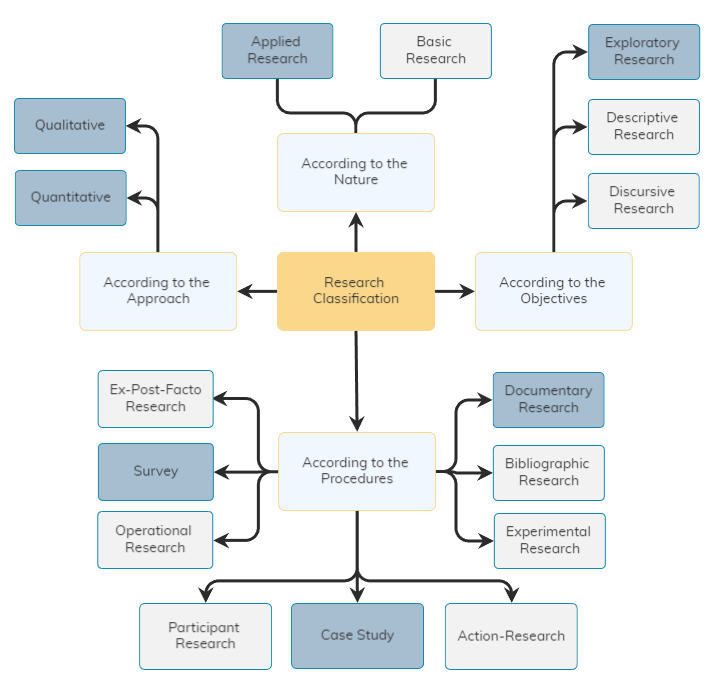
\includegraphics[width=14cm]{img/2-pesquisa-survey.png}
  \end{center}
  \fonte{Adapted from \cite{Prodanov:2013}.}
\end{figure}

\section{Research Design}\label{sec:met-design}

% Na \Cref{fig:research-design} está representada o fluxograma seguido no decorrer desta pesquisa, as atividades nele posicionadas estão divididas entre cinco fases:
In \Cref{fig:research-design} is represented the flowchart followed in the course of this research, the activities placed in it are divided into five phases:
\begin{inparaenum}[(1)]
  \item Information gathering;
  \item Partial development;
  \item Development;
  \item Evaluation;
  \item Publish.
\end{inparaenum}

% A primeira fase, \textbf{Information gathering}, é focada em organizar estruturas de pesquisa, questionarios, priorização de informações, aprendizado sobre o tema da pesquisa. Principalmente direcionada a produzir dois importantes artefatos da pesquisa, a revisão na literatura cinza e o survey com possíveis usuários finais.

The first phase, \textbf{Information Gathering}, is focused on organizing research structures, questionnaires, prioritization of information, and learning about the research topic. Mainly aimed at producing two important artifacts of the research, the review in the grey literature and the survey with possible end users.

% Seguindo para a segunda fase, \textbf{Partial Development}, onde foi decidido entre os envolvidos no projeto, que não seria viável implementar todo a ferramenta neste primeiro momento, então apenas algumas funcionalidades mais importantes e que ja seriam suficientes para um produto em estado inicial, seriam desenvolvidas.
% Dentro da fase de \textbf{Publish}, os dois Term Papers serão escritos e defendidos, ocorrendo de forma paralela ao desenvolvimento da ferramenta, majoritariamente acontecendo na fase de \textbf{Development}.

Moving on to the second phase, \textbf{Partial Development}, where it was decided among those involved in the project, that it would not be feasible to implement the entire tool at this first moment, so only some more important functionalities and that would already be sufficient for a \ac{MVP} \cite{Lenarduzzi:2016}, would be developed.
Within the \textbf{Publish} phase, the two \acp{TP} will be written and defended, occurring in parallel to the development of the tool, mostly happening in the \textbf{Development} phase.

% Após ja existir uma versão estável da ferramenta, onde usuários possam utiliza-la, esta será disponível para uso real, permitindo que um curso de extensão da Unipampa seja cadastrado e abrindo vagas para inscrições de participantes, com isto na fase de \textbf{Evaluation}, serão coletados os feedbacks, analisado os resultados e melhorias na ferramenta serão feitas.

After there is a stable version of the tool, where users can use it, it will be available for real use, allowing UNIPAMPA's outreach activities to be registered and opening vacancies for participant or volunteer registrations, with this in the phase of \textbf{Evaluation}, feedbacks will be collected, analyzed the results and improvements in the tool will be made.

\begin{figure}[htb]
  \caption{Research Design}\label{fig:research-design}
  \begin{center}
    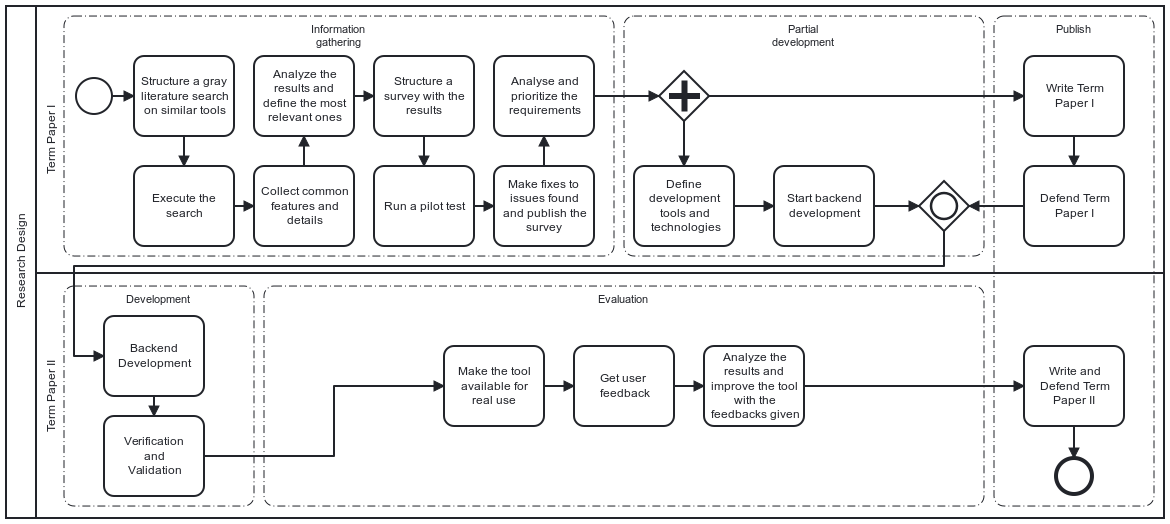
\includegraphics[width=16cm]{img/2-research-diagram.png}
  \end{center}
  \fonte{Author.}
\end{figure}

\section{Research Schedule}\label{sec:met-schedule}

% Para facilitar a visualização de como as atividades se deram ao decorrer do tempo, na \Cref{tbl:schedule} é apresentado todo o cronograma do que foi planejado desde o levantamento de informações até a defesa do Term Paper II.

To facilitate the visualization of how the activities took place over time. 
\Cref{tbl:schedule} presents the entire schedule of what was planned from the collection of information to the defense of \acl{TP} II.

\begin{table}[!htb]
  \centering
  \caption{Research Schedule}
  \label{tbl:schedule}
  \scriptsize
  \begin{tabular}{p{4cm}|l|lllll|lll}
    \bottomrule
    \rowcolor[rgb]{0.753,0.753,0.753} \multicolumn{1}{c|}{{\cellcolor[rgb]{0.753,0.753,0.753}}}                                       & \multicolumn{1}{c|}{\textbf{2021/2}} & \multicolumn{5}{c|}{\textbf{2022/1}} & \multicolumn{3}{c|}{\textbf{2022/2}}                                                                                                                                                                                                                                           \\
    \hhline{>{\arrayrulecolor[rgb]{0.753,0.753,0.753}}->{\arrayrulecolor{black}}---------|}
    \rowcolor[rgb]{0.753,0.753,0.753} \multicolumn{1}{c|}{\multirow{-2}{*}{{\cellcolor[rgb]{0.753,0.753,0.753}}\textbf{ Activities}}} & \textbf{Nov - Mar}                   & \multicolumn{1}{c}{\textbf{Apr}}     & \textbf{May}                         & \textbf{Jun}                         & \multicolumn{1}{l}{\textbf{Jul}}     & \textbf{Aug}                         & \textbf{Sep Oct Nov}                 & \textbf{Dec}                         & \multicolumn{1}{c|}{\textbf{Jan}}    \\
    \hline
    \rowcolor[rgb]{0.914,0.914,0.914} Plan and execute systematic review in the grey literature                                       & {\cellcolor[rgb]{0.753,0.753,0.753}} &                                      &                                      &                                      &                                      &                                      &                                      &                                      &                                      \\
    Plan and execute survey with target users                                                                                         &                                      & {\cellcolor[rgb]{0.753,0.753,0.753}} &                                      &                                      &                                      &                                      &                                      &                                      &                                      \\
    \rowcolor[rgb]{0.914,0.914,0.914} Analyze results from previous steps and map requirements                                        &                                      & {\cellcolor[rgb]{0.753,0.753,0.753}} & {\cellcolor[rgb]{0.753,0.753,0.753}} &                                      &                                      &                                      &                                      &                                      &                                      \\
    Plan and start tool development                                                                                                   &                                      &                                      & {\cellcolor[rgb]{0.753,0.753,0.753}} & {\cellcolor[rgb]{0.753,0.753,0.753}} &                                      &                                      &                                      &                                      &                                      \\
    \rowcolor[rgb]{0.914,0.914,0.914} Write Term Paper I                                                                              &                                      &                                      &                                      & {\cellcolor[rgb]{0.753,0.753,0.753}} & {\cellcolor[rgb]{0.753,0.753,0.753}} & {\cellcolor[rgb]{0.753,0.753,0.753}} &                                      &                                      &                                      \\
    Defend Term Paper I                                                                                                               &                                      &                                      &                                      &                                      &                                      & {\cellcolor[rgb]{0.753,0.753,0.753}} &                                      &                                      &                                      \\
    \rowcolor[rgb]{0.914,0.914,0.914} Continue the development of the tool                                                            &                                      &                                      &                                      &                                      &                                      & {\cellcolor[rgb]{0.753,0.753,0.753}} & {\cellcolor[rgb]{0.753,0.753,0.753}} & {\cellcolor[rgb]{0.753,0.753,0.753}} &                                      \\
    Execute a real use case on the tool                                                                                               &                                      &                                      &                                      &                                      &                                      &                                      &                                      & {\cellcolor[rgb]{0.753,0.753,0.753}} &                                      \\
    \rowcolor[rgb]{0.914,0.914,0.914} Write Term Paper II                                                                             &                                      &                                      &                                      &                                      &                                      &                                      &                                      & {\cellcolor[rgb]{0.753,0.753,0.753}} & {\cellcolor[rgb]{0.753,0.753,0.753}} \\
    Defend Term Paper II                                                                                                              &                                      &                                      &                                      &                                      &                                      &                                      &                                      &                                      & {\cellcolor[rgb]{0.753,0.753,0.753}} \\
    \toprule
  \end{tabular}
  \fonte{Author.}
\end{table}


\section{Chapter Summary}\label{sec:met-summary}

% Neste capitulo foi apresentado o significado de metodologia, e como ela pode ser classificada dentro de um ambito cientifico, juntamente com quais termos que se aplicam ao presente Term Paper. Além disso foi apresentado o design de pesquisa contendo os passos realizados pelo autor, como também os que serão dados.

In this chapter we have presented the meaning of methodology, and how it can be classified within a scientific scope, along with what terms apply to this \ac{TP}. 
In addition, the research design was presented containing the steps taken by the author, as well as those that will be given.

%------------------------------------------------------------------------------

%------------------------------------------------------------------------------
% Migrar o anteprojeto
%  Falar sobre a literatura cinza para identificar as ferramentas, atualizar a figura
%  Atualizara imagem colocar o survey e na classificaç~ao de pesquisa adicionar o survey. Retirar pesquisa documental
%  Olhar os outros TCCs para exemplo
%  Detalhar mais o que é cada caixa do desenho de pesquisa
%  Detalhar mais cada caixinha da figura 3
% Imagens: Cronograma desde 2021/2, atualizar (segundo semestre vai ate julho) (prox ano comeca em julho e vai ate janeiro) 
  % 20/07
% Fundamentação Teórica (Background) - CAP de extensão universitaria, CAP de curricularização da extensão, soluções/ferramentas de apoio a extensão (spoiler) se basear nas leis federais, resoluç~oes da unipampa (se aprofundar na previa do antreprojeto) como que a extensão funciona no Brasil, como é implantada nas universidades, o que foi a lei de curricularização, capitulo para falar da unipampa cidadã (Geral sobre extensão, tipos, perfis de pessoas, sempre com funcamentação. Programas e projetos de extensão na Unipampa (para demonstrar como é importante dentro da faculdade, impacto da ferramenta, graficos, valores)

%==============================================================================
\chapter{BACKGROUND}\label{background}
%==============================================================================
% 1 ou 2 paragrafos 

% ============================================================================
% Neste capitulo são discutidos assuntos assuntos que complementam o objetivo do presente trabalho, ajudando no entendimento das politicas e resoluções envolvidas. 
% Na \Cref{sec:3.1} sera apresentada a politica nacional de extensão, que vale para todo o Brasil sobre os objetivos que a extensão universitária tem em relação a comunidade academica e externa. 
% Logo em seguida na \Cref{sec:3.2} a visão de como a Unipampa se adaptou para receber estas novas regras. 
% Após, na \Cref{sec:3.2.1} a diferenca entre programas e projetos de extensão sera apresentada, seguido por uma explicação mais detalhada sobre o projeto 'Unipampa Cidadã' na \Cref{sec:3.2.2}. 
% A \Cref{sec:3.3} releva algumas ferramentas relacionadas ao assunto do trabalho, seus pontos em comum e uma descrição em alto nível. 
% Por fim na \Cref{sec:3.4} um resumo geral sobre o capitulo é apresentado.

This chapter discusses subjects that complement the objective of this work, helping to understand the policies and resolutions involved.
In \Cref {sec:3.1} the national outreach activity policy will be presented, which is valid for all of Brazil on the objectives that university outreach has in relation to the academic and external community.
Then in \Cref{sec:3.2} the vision of how Unipampa has adapted to receive these new rules.
After that, in \Cref {sec:3.2.1} the difference between outreach programs and projects will be presented, followed by a more detailed explanation about the ``Unipampa Cidadã'' project in \Cref{sec:3.2.2}.
The \Cref{sec:3.3} highlights some tools related to the subject of the work, their commonalities and a high-level description.
Finally in \Cref{sec:3.4} a general summary of the chapter is presented.
% ============================================================================

\section{National Outreach Policy}\label{sec:3.1}
% Descrever a politica em si
% ============================================================================
% Sabemos que a extensão universitária é uma area de grande importancia para a comunidade academica e externa, também sendo uma ferramenta de conexão entre professores, alunos e população, tendo muito impacto na formação de um estudante. 
% Para fortalecer os objetivos que a extensão universitaria tem dentro deste universo, o Fórum de Pró-Reitores de Extensão das Universidades Públicas Brasileiras (FORPROEX), acrescentou a versão antiga do documento da Politica Nacional de Extensão, publicado em 1999, com situações atuais e desafios encontrados nos ultimos anos. 
% A nova versão do documento, \cite{politicaNacional}, dentro dos seus objetivos, temos como exemplo os que seguem:

It is well-known that university outreach is an area of great importance for the academic and external community, also being a tool for connecting professors, students and the population, having a great impact on the formation of a student. 
To strengthen the objectives that university extension has within this universe, the \acl{FORPROEX} (\ac{FORPROEX}), updated the old version of the National Outreach Policy document, published in 1999, with current situations and challenges found in recent years.
The new version of the document, \cite{politicaNacional}, within its objectives, has as an example the following:
% ============================================================================

% ============================================================================
% \begin{itemize}
%     \item Conquistar o reconhecimento da extensão universitária, como uma ferramenta essencial para a universidade pública.
%     \item Garantir que a extensão seja a solução para qualquer tipo de problema social enfrentado pelo país.
%     \item Defender o financiamento de programas e projetos de extensão para que estes mantenham o seu funcionamento.
%     \item Promover a conscientização ambiental e sustentavel em projetos extensionistas no Brazil.
%     \item Além de nacionalmente, promover a solidariedade internacionalmente, abrangindo a aréa de impacto das ações extensionistas.
% \end{itemize}

\begin{itemize}
    \item Achieve the recognition of university outreach activities as an essential tool for the public university;
    \item Ensure that the outreach activity is the solution to any type of social problem faced by the country;
    \item Defend the funding of outreach programs and projects so that they can continue to function;
    \item Promote environmental and sustainable awareness in outreach projects in Brazil;
    \item Promote solidarity both nationally and internationally, covering the area of impact of outreach actions.
\end{itemize}
% ============================================================================

% ============================================================================
% Servindo como base para as universidades, o documento ``Referenciais para a construção de uma Política Nacional de Extensão nas ICES'' \cite{referenciaisPolitica}, 
% discute um pouco sobre a duvida da classificação de uma atividade academica como extensionista ou não, mas deixando como fato a seguinte frase ``Se a dimensão teórica da Extensão tende à maior rigidez - no sentido que precisa guardar princípios, retomar referenciais, 
% dialogar com outros documentos institucionais – a dimensão prática possibilita maior flexibilidade, originando uma considerável diversidade de ações''. 
% Este documento também destaca a importancia da integração da extensão com a pesquisa e ensino, com discussões de cunho social e efeitos dos resultados na sociedade.

Serving as a basis for universities, the document ``Referentials for the construction of a National Outreach Policy in \aclp{ICES} (\ac{ICES})'' \cite{referenciaisPolitica},
discusses a little about the doubt of classifying an academic activity as outreach or not, but leaving as a fact the following sentence ``If the theoretical dimension of university outreach tends towards greater rigidity - in the sense that it needs to keep principles, resume references,
dialogue with other institutional documents – the practical dimension allows for greater flexibility, giving rise to a considerable diversity of actions''.
This document also highlights the importance of integrating extension with research and teaching, with discussions of a social nature and the effects of the results on society.
% ============================================================================

% ============================================================================
% No documento supracitado, conjuntamente são aprofundados nove tipos de ações de extensão possíveis, cada um com suas peculiaridades, dividindo-as  em ações diretas de extensão e ações que permitem a integração entre extensão e ensino e extensão e pesquisa. 

In the aforementioned document, nine types of possible \acp{OA} are discussed in depth, each with its peculiarities, dividing them into direct outreach actions and actions that allow the integration between outreach and teaching or outreach and research.

% ============================================================================

%https://sites.unipampa.edu.br/proext/documentos/politica-nacional-de-extensao/
% Plano Nacional de Educação 2014-2024 (Lei 13.005/2014)
% https://curricularizacaodaextensao.ifsc.edu.br/files/2016/06/1_Artigo_Curricularizaca_da_Extensao_Universitaria_no_Brasil.pdf
% FOREXT. Extensão nas Instituições Comunitárias de Ensino Superior: referenciais para a construção de
% uma Política Nacional de Extensão nas ICES (2013). Recuperado em 12 de março, 2015, em
% <http://www1.pucminas.br/imagedb/documento/DOC_DSC_NOME_ARQUI20150309182334.pdf>
% FORPROEX. Política Nacional de Extensão Universitária (2012). Recuperado em 12 de outubro, 2014,
% de <http://www.renex.org.br/documentos/2012-07-13-Politica-Nacional-de-Extensao.pdf>

\subsection{\acl{OA} Curricularization in Higher Education}\label{sec:3.1.1}
% Descrever aqui a ideia geral de como implementar isso dentro dos cursos pelas diferentes IESs
% ============================================================================
% Entrando no âmbito do ensino superior foi criado a Resolução Nº 7, de 18 de Dezembro de 2018 \cite{ministerioSuperiorExtensao}, aonde ela instituí diretrizes, princípios, fundamentos e procedimentos para a extensão na educação superior brasileira.
% Desta maneira foi regulamentado que as atividades de extensão serão disponibilizadas na forma de componentes curriculares para os cursos.

Entering the scope of higher education, Resolution No. 7, of December 18, 2018 \cite{ministerioSuperiorExtensao} was created, where it established guidelines, principles, foundations and procedures for university outreach in Brazilian higher education.
In this way, it was regulated that the \acp{OA} will be made available in the form of curricular components for the courses.
% ============================================================================

% ============================================================================
% Neste documento também é determinado que as atividades de extensão devem compor no minimo 10\% (dez por cento) de toda a carga horária dos cursos de graduação, sendo elas caracterizadas como uma atividade intervencionista que envolva diretamente a comunidade externa e esteja relacionada com a formação estudantil.

In this document, it is also determined that \acp{OA} must make up at least 10\% (ten percent) of the entire workload of undergraduate courses, being characterized as an interventionist activity that directly involves the external community and is related to student training.
% ============================================================================

% ============================================================================
% Outro ponto importante levantado, tem relação com a autoavaliação das atividades de extensão, para ocorrer ao aperfeicoamento constante da mesma. Nesta avaliação deverá ser incluido a identificação da pertinência da utilização das atividades de extensão na
% creditação curricular, a contribuição para o cumprimento dos objetivos do Plano de Desenvolvimento Institucional e dos Projetos Pedagógico dos Cursos e por fim a apresentação dos resultados conquistados em relação ao público participante.

Another important point raised is related to the self-assessment of outreach activities, in order to constantly improve it. 
This evaluation should include the identification of the relevance of the use of \acp{OA} in curricular accreditation, the contribution to the fulfillment of the objectives of the \ac{IDP} and the Pedagogical Projects of the Courses and, finally, the presentation of the results achieved in relation to the participating public.
% ============================================================================

% ============================================================================
% Todas as atividades de extensão também deverão ser registradas conforme as regras citadas na mesma resolução \cite{ministerioSuperiorExtensao}, devendo conter o planejamento de suas atividades internas, as estratégias para a autoavaliação, proposta, desenvolvimento e conclusão, estes devem estar devidamente registrados e analisados para poder ser feito a organização de seus planos de trabalho. 

All \acp{OA} must also be registered according to the rules mentioned in the same resolution \cite{ministerioSuperiorExtensao}, and must contain the planning of their internal activities, strategies for self-assessment, proposal, development and conclusion, these must be duly registered and analyzed in order to be able to organize your work plans.
% ============================================================================

% ============================================================================
% Por fim, a resolução supramencionada determina que ``As instituições de ensino superior terão o prazo de até 3 (três) anos, a contar da data de sua homologação, para a implantação do disposto nestas Diretrizes.''

Finally, the aforementioned resolution determines that ``Higher education institutions will have a period of up to 3 (three) years, counting from the date of their approval, to implement the provisions of these Guidelines.''
% ============================================================================

\section{\acl{OA} Curricularization in \acl{UNIPAMPA}} \label{sec:3.2}
% Descrever a visão da unipampa 
% https://sites.unipampa.edu.br/proext/documentos/normas-de-extensao-da-unipampa/
% https://sites.unipampa.edu.br/proext/files/2021/05/res-317_2021-politica-de-extensao.pdf
% - RESOLUÇÃO CONSUNI/UNIPAMPA Nº 317, DE 29 DE ABRIL DE 2021
% https://sites.unipampa.edu.br/proext/files/2021/12/sei_unipampa-0700488-resolucao-consuni.pdf
% - RESOLUÇÃO CONSUNI/UNIPAMPA Nº 332, DE 21 DE DEZEMBRO DE 2021

% Citar os cases de sucesso como ES e outros cursos de Uruguaiana

% ============================================================================
% Estando na visão da Unipampa, ela como todas as universidades federais, deve ter uma resolução voltada para a normatização para as atividades de extensão de modo geral apresentando o que elas são, seu publico alvo, objetivos etc. 
% Tendo em vista isso a Unipampa na Resolução CONSUNI/UNIPAMPA Nº 332 de 2021, \cite{Resolucao-332:2021}, determina os tipos de atividades de extensão, ja mencionados na \Cref{introduction}, seus orgãos gerenciadores, equipe executora, possíveis processos relacionados, e algumas regras como a de duração mínima de 8 (oito) horas, levando-se em conta o período de organização, execução e elaboração de relatório final.

In \ac{UNIPAMPA}'s view, like all other \acl{HEI}, must have a resolution aimed at standardizing \acp{OA} in general, presenting what they are, their target audience, objectives, etc.
In view of this, \ac{UNIPAMPA}, in CONSUNI/UNIPAMPA Resolution No. 332 of 2021, \cite{Resolucao-332:2021}, determines the types of extension activities, already mentioned in \Cref{introduction}, its managing bodies, executing team, possible related processes, and some rules such as the minimum duration of 8 (eight) hours, taking into account the period of organization, execution and preparation of the final report.
% ============================================================================

% ============================================================================
% A algum tempo a Unipampa ja vem implantando alguns projetos de extensão dentro de sua grade curricular, por exemplo no curso de Engenharia de Software onde dentro da cadeira de Resolução de Problemas, os alunos se reunem em grupos, semelhante a times de desenvolvimento e gerencia de projetos, sendo eles designados para trabalhar em uma demanda real para alguém da comunidade externa. 
% Esta atividade proporciona ao aluno uma experiência muito recompensadora, pela oportunidade de falar, interagir e contribuir diretamente com um cliente que necessita de ajuda na resolução de algum problema.

For some time now, \ac{UNIPAMPA} has been implementing some outreach projects within its curriculum, for example in the Software Engineering course where, within the Problem Solving subject, students meet in groups, similar to development teams and project management, where they are assigned to work on real demand for someone in the external community.
This activity provides the student with a very rewarding experience, for the opportunity to talk, interact and contribute directly with a customer who needs help in solving a problem.

% ============================================================================

% ============================================================================
% Os principais objetivos na inserção das atividades extensionistas nos cursos de graduação, que a Unipampa ressalta em sua Resolução Nº 317 de 2021, \cite{CONSUNI-Unipampa:2021} são os seguintes: 
% \begin{itemize}
%   \item Ajudar ao discente desenvolver sua formação crítica, cidadã, interdisciplinar e responsável;
%   \item Aprimorar como um todo o ensino nos cursos de graduação e fortalecer aa indissociabilidade entre ensino, pesquisa e extensão;
%   \item Fortalecer o compromisso social da Unipampa; 
%   \item Estimular discussões construtivas em todos os setores da Unipampa; 
%   \item Promover ações que fortifiquem os princípios éticos, e o compromisso social da Unipampa em todas as áreas;
%   \item Instigar a comunidade academica a estar mais presente no desenvolvimento humano, academico, social, cultural e economico.
% \end{itemize}

The main objectives in the insertion of outreach activities in undergraduate courses, which \ac{UNIPAMPA} highlights in its Resolution No. 317 of 2021, \cite{CONSUNI-Unipampa:2021} are the following:
\begin{itemize}
  \item Help students develop their critical, citizen, interdisciplinary and responsible education;
  \item Improve teaching in undergraduate courses as a whole and strengthen the inseparability between teaching, research and outreach;
  \item Strengthen \ac{UNIPAMPA}'s social commitment;
  \item Stimulate constructive discussions in all sectors of \ac{UNIPAMPA}; 
  \item Promote actions that strengthen \ac{UNIPAMPA}'s ethical principles and social commitment in all areas;
  \item Encourage the academic community to be more present in human, academic, social, cultural, and economic development.
\end{itemize}
% ============================================================================

\subsection{Outreach Programs and Projects}\label{sec:3.2.1}
% Diferença entre eles
% Citar exemplos de Prog. e Proja. dos cursos do campus

% ============================================================================
% Para explicar o que são programas e projetos de extensão, sera utilizado as definições da \citeonline{referenciaisPolitica}, este diz que são atividades reguladas internamente pela instituição que articula eventos envolvendo ensino e pesquisa, sempre envolvendo a comunidade externa. 
% Com eles os alunos podem tomar atitudes e decisões diretamente sobre a comunidade em que vive, contribuindo na evolução e progresso da mesma. 
% Além de ajudar a comunidade externa, \ac{FOREXT} diz que os programas e projetos não buscam criar um laço de dependência com a universidade, sendo assim é necessário resolver o problema com mais eficácia e qualidade possível.

To explain what outreach projects and programs are, the definitions of \citeonline{referenciaisPolitica} will be used, which says that they are activities regulated internally by the institution that articulates events involving teaching and research, always involving the external community.
With them, students can take attitudes and decisions directly about the community in which they live, contributing to its evolution and progress.
In addition to helping the external community, \ac{FOREXT} says that the programs and projects do not seek to create a bond of dependence with the university, so it is necessary to solve the problem with the most efficiency and quality possible.

% ============================================================================

% ============================================================================
% Pelo fato dos dois termos serem semelhantes, alguma confusão pode acontecer, então \citeonline{Viero} destaca a diferença entre os dois, citando as definições feitas pela \ac{ProExt}:

Because the two terms are similar, some confusion can arise, so \citeonline{Viero} highlights the difference between the two, citing the definitions made by \ac{ProExt}:
% ============================================================================

% ============================================================================
% \begin{citacao}
% É importante salientar que o ProExt prevê dois conjuntos de ações de extensão universitária: projetos de extensão, definidos como “conjunto de ações processuais contínuas, de caráter educativo, social, cultural ou tecnológico, com objetivo específico e prazo determinado”; e programa de extensão, como “conjunto articulado de projetos e outras ações de extensão, preferencialmente de caráter multidisciplinar e integrado a atividades de pesquisa e de ensino \cite{Viero}
% \end{citacao}

\begin{citacao}
It is important to point out that ProExt provides for two sets of university outreach actions: outreach projects, defined as “a set of continuous procedural actions, of an educational, social, cultural or technological nature, with a specific objective and a determined period”; and outreach program, as “an articulated set of projects and other outreach actions, preferably of a multidisciplinary nature and integrated with research and teaching activities \cite{Viero}.
\end{citacao}
% ============================================================================

% ============================================================================
% Dentro da \ac{UNIPAMPA} campus Alegrete existem alguns projetos e programas vigentes, são exemplos deles com os seus respectivos coordenadores: 
% \begin{inparaenum}[(1)]
%   \item \textbf{Ciência a Cavalo: Universidade e Ensino Básico de Mãos Dadas pelo Fortalecimento da Educação}, Marco Antonio Durlo Tier;
%   \item \textbf{Consultoria de TI para empresas do agronegócio}, Elder de Macedo Rodrigues;
%   \item \textbf{Empresa Júnior: Multi Assessoria e Soluções em Engenharia Júnior - Masé Junior}, José Gabriel Vieira Neto;
%   \item \textbf{Espaço Maker} - Aprendizagem criativa, Vitor Almada;
%   \item \textbf{Programa UniHacker.Club}, Diego Luiz Kreutz;
%   \item \textbf{UNIPATAS Alegrete: Proteção, Esterilização e Adoção}, Camila da Costa Lacerda Tolio Richardt;
%   \item \textbf{Programa C}, Aline Vieira de Mello;
%   \item \textbf{Programa JEDI}, Maicon Bernardino da Silveira.
% \end{inparaenum}

% ########################
% Professor, fiquei em dúvida se traduzia os nomes dos programas de extensão, dai eu traduzi so o que eu achei que não fazia parte do nome em si.
% ########################
Within the \ac{UNIPAMPA} Alegrete campus there are some current projects and programs, examples of which are with their respective coordinators:
\begin{inparaenum}[(1)]
  \item \textbf{Ciência a Cavalo: University and Basic Education Hand in Hand for Strengthening Education}, Profº Marco Antonio Durlo Tier;
  \item \textbf{IT consultancy for Agribusiness Companies}, Profº Elder de Macedo Rodrigues;
  \item \textbf{Empresa Júnior: Multi Advisory and Solutions in Junior Engineering - MASE Junior}, Profº José Gabriel Vieira Neto;
  \item \textbf{Espaço Maker} - Criative Learning, TAE Vitor Almada;
  \item \textbf{Programa UniHacker.Club}, Profº Diego Luiz Kreutz;
  \item \textbf{UNIPATAS Alegrete: Protection, Sterilization and Adoption}, TAE Camila da Costa Lacerda Tolio Richardt;
  \item \textbf{Programa C}, Profª Aline Vieira de Mello;
  \item \textbf{Programa JEDI}, Profº Maicon Bernardino da Silveira.
\end{inparaenum}
% ============================================================================

% ============================================================================
% Utilizando a página online do ultimo programa citado \citeonline{JEDI}, este é um programa que se propoe a resolver problemas locais utilizando tecnologia e envolvimento com a comunidade. 
% No primeiro ciclo do programa quatro projetos de extensão foram propostos, cada um com seus objetivos, metodologias e atividades próprios, são eles:
% \begin{inparaenum}[(1)]
%   \item Padawan Academy;
%   \item Jedi Apprentice;
%   \item Jedi Problem-Solving;
%   \item Jedi Mind.
% \end{inparaenum}

% Using the online page of the last mentioned program \citeonline{JEDI}, this is a program that proposes to solve local problems using technology and community involvement.
% In the first cycle of the program, four outreach projects were proposed, each with its own objectives, methodologies and activities, they are:
% \begin{inparaenum}[(1)]
%   \item Padawan Academy;
%   \item Jedi Apprentice;
%   \item Jedi Problem-Solving;
%   \item Jedi Mind.
% \end{inparaenum}

% ============================================================================

\subsection{Processes for New Proposals for Outreach Programs and Projects}

% ============================================================================
% Para ser realizado o novo cadastro de um programa ou projeto de extensão e sua geração de certificados ao final, existem algumas normas definidas pela \citeonline{Resolucao-332:2021}, que devem ser desempenhados antes. 
% Tendo em maos estes documentos a \ac{UNIPAMPA} normatizou alguns esquemas de fluxo dos processos, para que todos os proponentes tenham conhecimento do que acontece depois que a proposta é realizada.

In order to register a new outreach program or project and generate certificates at the end, there are some rules defined by \citeonline{Resolucao-332:2021}, which must be performed beforehand.
With these documents in hand, \ac{UNIPAMPA} standardized some process flow schemes, so that all proponents are aware of what happens after the proposal is made.
% ============================================================================

% ============================================================================
% Na \Cref{fig:outreach-projects-registration}, o fluxo de cadastro de um novo projeto de extensão é apresentado, nele é possivel ver que a proposta passa por diversos passos de correções e avaliações, sendo enviada para diversos atores ao longo do processo.
% Por fim sendo decisão da \ac{PROEXT} solicitar alterações finais, ou homologar o projeto, deferindo um novo número de registro.

In \Cref{fig:outreach-projects-registration}, the registration flow of a new outreach project is presented, in which it is possible to see that the proposal goes through several steps of corrections and evaluations, being sent to several actors throughout the process.
% ============================================================================

\begin{figure}[htb]
  \caption{Outreach Projects Registration}\label{fig:outreach-projects-registration}
  \begin{center}
    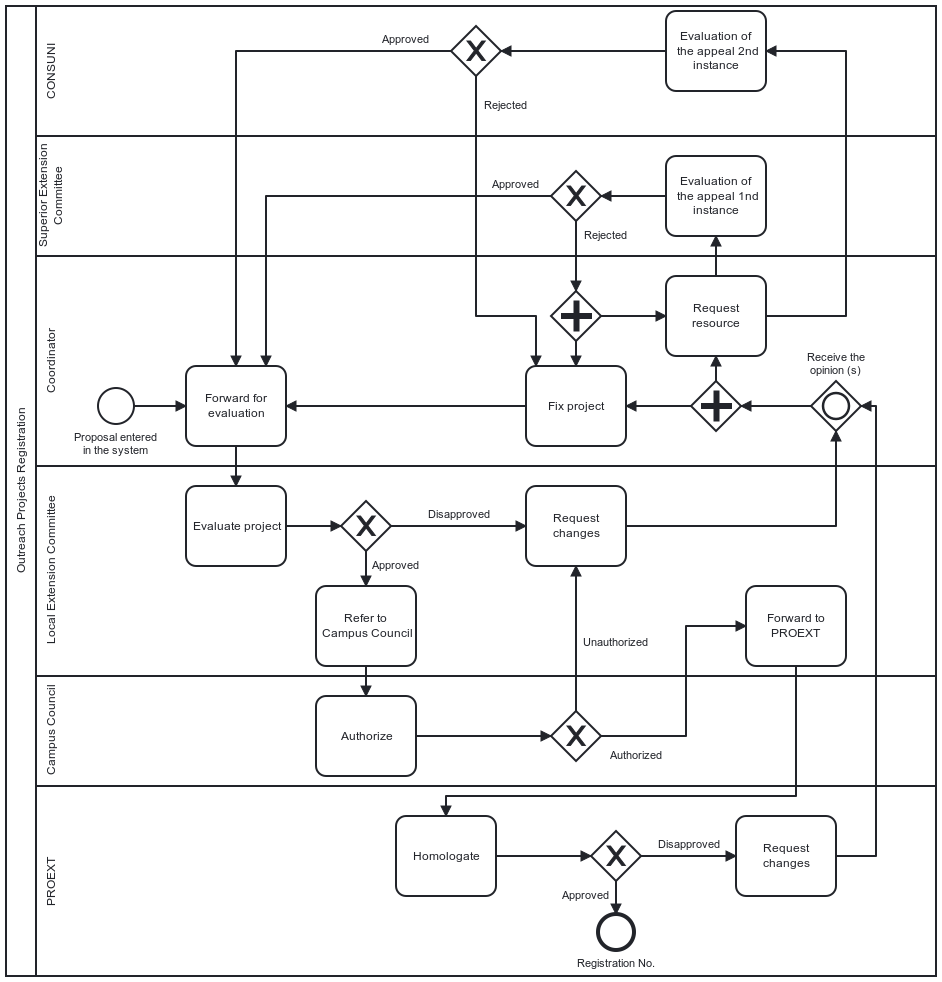
\includegraphics[width=16cm]{img/3-registro-de-projetos-de-extensao.png}
  \end{center}
  \fonte{Adapted from \cite{siteProcessos}.}
\end{figure}

% ============================================================================
% Já na \Cref{fig:issuance-certificates}, estão representados os passos relacionados a homologação e geração de certificados, comecando com o proponente da atividade tendo em maõs a lista de presença e a planilha com informações para a geração dos certificados, logo um relatorio final é construido e inserido no sistema \ac{SIPPEE}, este é avaliado e homologado, chegando novamente até a \ac{PROEXT} que com a planilha enviada, envia seus dados para o sistema \ac{SGCE}, recebendo os certificados e os enviando para os emails dos participantes. 

In the \Cref{fig:issuance-certificates}, the steps related to the approval and generation of certificates are represented, starting with the proponent of the activity having the attendance list and the spreadsheet with information for the generation of certificates. 
Then, a final report is built and inserted in the \ac{SIPPEE} system, it is evaluated and approved, reaching again at \ac{PROEXT} which, with the spreadsheet sent, sends its data to the \ac{SGCE} system, receiving the certificates and sending them to participants' emails.
% ============================================================================

\begin{figure}[htb]
  \caption{Issuance of certificates}\label{fig:issuance-certificates}
  \begin{center}
    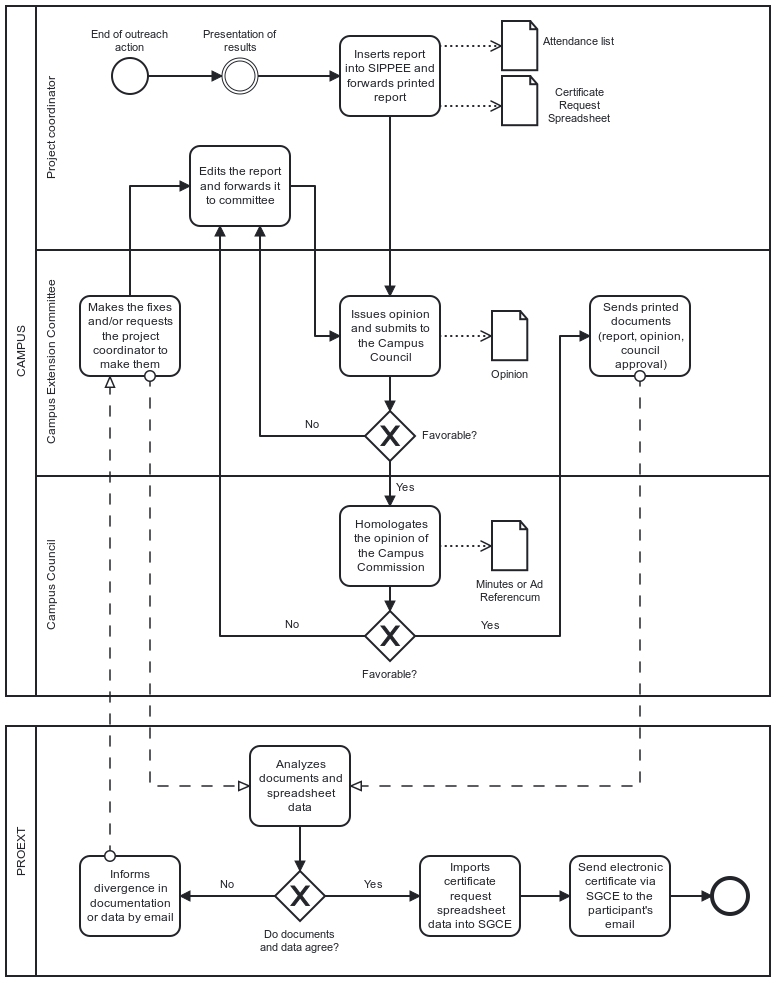
\includegraphics[width=16cm]{img/3-emissao-de-certificados.png}
  \end{center}
  \fonte{Adapted from \cite{siteProcessos}.}
\end{figure}

\subsection{``Unipampa Cidadã'' Program}\label{sec:3.2.2}
% https://unipampa.edu.br/portal/sites/default/files/documentos/instrucao_normativa_18-2021_revoga_in-17-2021_normatiza_o_programa_institucional_unipampa_cidada.pdf
% INSTRUÇÃO NORMATIVA UNIPAMPA Nº 18, 05 DE AGOSTO DE 2021

% ============================================================================
% A \ac{UNIPAMPA} atravez da Instrução Normativa Nº 18 \cite{unipampacidada}, usando a Resolução Nº317 \cite{CONSUNI-Unipampa:2021}, foi estabelecido que o projeto de extensão chamado "UNIPAMPA Cidadã" deverá ser ofertado por todos os cursos, sendo composto por atividades de cidadania e solidariedade e com o objetivo de  formar egressos cientes de sua responsabilidade social, estimulando e aumentando a integração com a comunidade local.

\ac{UNIPAMPA} through Normative Instruction No. 18 \cite{unipampacidada}, using Resolution No.317 \cite{CONSUNI-Unipampa:2021}, established that the outreach project called ``Unipampa Cidadã'' must be offered by all courses, consisting of citizenship and solidarity activities and with the objective of training graduates aware of their social responsibility, stimulating and increasing integration with the local community.
% ============================================================================

% ============================================================================
% Após a implementação do projeto nos cursos da instituição, esta deverá ser realizada por todos os discentes, a cadeira ofertada para o projeto deverá ter no mínimo 60 e no máximo 120 horas. 
% As ações comunitárias devem ser realizadas em instituições públicas, \acp{NGO} e organizações ou associações da sociedade civil organizada. O supervisor de extensão do curso é o encarregado por fazer a avaliação do projeto, planejamento, acompanhamento, validação e ele será responável por aprovar o inicio das atividades.

After the implementation of the project in the institution's courses, it must be carried out by all students, the course offered for the project must have a minimum of 60 and a maximum of 120 hours.
Community actions must be carried out in public institutions, \acp{NGO} and organizations or associations of organized civil society. 
The course extension supervisor is responsible for carrying out the project evaluation, planning, monitoring, validation and he will be responsible for approving the beginning of the activities.
% ============================================================================

% ============================================================================
% O projeto também disponibiliza na Instrução Normativa Nº 18, um modelo de formulário para preenchimento de dados quando as atividades são finalizadas, permitindo o discente refletir sobre o impacto do projeto sob sua visão apontando seus aprendizados durante a execução. 
% Por fim o supervisor pode realizar observaçoes sobre o discente e indicar se este foi aprovado ou reprovado.

The project also makes available in Normative Instruction Nº 18, a form template for filling in data when the activities are completed, allowing the student to reflect on the impact of the project under their view, pointing out what they learned during the execution.
Finally, the supervisor can make observations about the student and indicate whether he or she passed or failed.
% ============================================================================
\section{Similar Outreach Support Tools}\label{sec:3.3}
% Overview de soluções
% Descrever em alto nível e fazer gancho (spoiler) com o Capítulo do grey
% Funcionalidades comuns
% Foi feito um detalhamento metodologico no capitulo 4.1
% Tentamos fazer revisão sistematica, encontramos duas mas preferimos a cinza
% Citar artigos que falam do ferramental

% ============================================================================
% Em conjunto com o \Cref{cap:grey} que ira apresentar a revisão conduzida na literatura cinza, algumas ferramentas foram pesquisadas para adiquirir informaçoes de como o mercado está em relaçao a extensão nas universidades. 
% Com os resultados foi possível levantar funcionalidades, detalhes e pontos em comum dentre as ferramentas.

In conjunction with \Cref{grey_literature} that will present the review conducted in the grey literature, some tools were researched to acquire information on how the market is in relation to outreach in universities.
With the results it was possible to raise functionalities, details and common points among the tools.
% ============================================================================

% ============================================================================
% Em um primeiro momento os autores buscaram fazer uma revisão sistematica na literatura branca, mas os resultados encontrados não satisfazeriam por completo, visto que a exploração manual por várias ferramentas relacionadas ao tema, traria mais conteúdo para ser classificado e discutido entre os envolvidos na pesquisa.

At first, the authors sought to make a systematic review of the white literature, but the results found would not be completely satisfactory, since the manual exploration by various tools related to the topic would bring more content to be classified and discussed among those involved in the research.
% ============================================================================

% ============================================================================
% Durante a execução da revisão, a ferramenta que mais retornou resultados e estava sempre presente nas pesquisas, foi a \ac{SIGAA}, a qual é a mais utilizada por diversas instituições, sendo ela muito completa contendo partes em seu sistema voltados para a maioria dos processos que envolvem uma instituição. 
% Outra que apresentou resultados interessantes foi a \ac{CAEX}, que apresentou diversas funcionalidades únicas, sendo apenas ela que as apresentava, com ela foi possível retirar ideias de grande importancia para a construção de uma ferramenta completa.

During the execution of the review, the tool that returned the most results and was always present in the research was \ac{SIGAA}, which is the most used by several institutions, being very complete, containing parts in its system aimed at most processes involving an institution.
Another one that presented interesting results was \ac{CAEX}, which presented several unique features, being only it that presented them, with this it was possible to extract ideas of great importance for the construction of a complete tool.
% ============================================================================
\section{Chapter Summary}\label{sec:3.4}
% ============================================================================
% Neste capítulo foi apresentado diretrizes de varias resoluçoes e normativas relacionadas a extensão, tanto no pais como um todo, quanto na \ac{UNIPAMPA}. 
% Também foi discutido sobre as semelhanças e diferenças entre os termos programa e projeto de extensão, apresentando os processos mais relevantes envolvidos no seu periodo de vida.
% Como exemplo mais recente de programa de extensão, a "UNIPAMPA Cidadã" teve parte de seus objetivos e diretrizes apresentados, por fim foi discutido um pouco sobre a revisão na literatura cinza executada pelos participantes desta pesquisa, logo no proximo capítulo será mais aprofundado critérios, metodologia, resultados, questões de pesquisa, dentre outras informaçoes pertinentes a literatura cinza.

In this chapter, guidelines of various resolutions and regulations related to extension were presented, both in the country as a whole and in \ac{UNIPAMPA}.
It was also discussed the similarities and differences between the terms outreach program and project, presenting the most relevant processes involved in its life span.
As a more recent example of an extension program, ``Unipampa Cidadã'' had part of its objectives and guidelines presented, finally, a little discussion about the grey literature review carried out by the participants of this research was discussed, so in the next chapter, criteria will be more in-depth, methodology, results, research questions, among other information relevant to grey literature.
% ============================================================================   % 20/07
%==============================================================================
\chapter{GREY LITERATURE}\label{grey_literature}
%==============================================================================

Before beginning to develop the solution itself, it would be extremely beneficial to conduct a systematic review of the grey literature to map and assess existing tools and solutions that already address the issue of managing outreach activities in the context of \acp{HEI}. This research will ultimately result in a software product. Two authors did the review. Although the two \ac{TP} were prepared independently, as was already indicated, the artifacts produced to support the study were produced collectively.

The systematic review of the grey literature is described in this chapter. Additionally, data gathered during the study that is pertinent to the creation of the target product will be presented. In addition to a thorough examination and comparison of the chosen tools, the protocol established to conduct the evaluation will be covered, citing details such research questions, inclusion and exclusion criteria, extracted data, and search strings.

In this manner, the chapter is structured in the following way: Introduced in the \Cref{sec:gl-background} are words and ideas utilized in the study. The technique outlined by the authors will be presented in \Cref{sec:gl-planning}. The methods used in the study and the information gathered to address the research questions will be explained in the \Cref{sec:gl-reporting}, while the \Cref{sec:gl-validity} highlights risks to the study's validity. The systematic review is concluded by \Cref{sec:gl-considerations}.

\section{Background}\label{sec:gl-background}

The following definition of grey literature comes from \textcite[p.2]{garousi2019guidelines}:
\begin{citacao}
  <grey literature> is produced at all levels of government, academia, business, and industry in print and electronic formats, but is not controlled by commercial publishers, or that is, where publication is not the main activity of the producing body.
\end{citacao}

The quality of software described as a ``black box'' is one in which the internal workings of the system are unknown; its use solely concentrates on the outputs produced in response to chosen inputs and execution conditions \textcite{nidhra2012black}.

This description was used in relation to the Google search engine, where it is unknown exactly what occurs internally other than the fact that occasionally, despite the identical search word, the results differ just little.

\section{Planning}\label{sec:gl-planning}

Due to the limited amount of formal works published on the issue of outreach activities management, the authors determined that a systematic review of the grey literature would be more interesting and valuable to the study than one in the white literature.

\subsection{Reasons for Carrying out the Review}\label{sec:gl-planning-motives}

The following were the key justifications given by the authors to include a review of grey literature in their study:
\begin{inparaenum}[(i)]
    \item More tools than formal articles in search results;
    \item Very few results were obtained when the search terms were applied to white literature;
  \item There are a number of tools and solutions without published articles;
  \item The authors are looking for tools in order to gather functionality ideas and inspiration for the creation of the intended product.
\end{inparaenum}

The questions and their responses that were used to make the choice to conduct the review of the grey literature can be found in \Cref{tab:questoesgarousi}. Additionally, the following objectives were specified for carrying out the review:

\begin{inparaenum}[(i)]
  \item Find free tools that partially support academic management;
  \item Find features in existing tools;
  \item Validate ideas for features and data that will be used in the solution.
\end{inparaenum}

\begin{table}[!htb]
  \centering
  \caption{Questions for Inclusion of Grey Literature}
  \label{tab:questoesgarousi}
  \footnotesize
  \begin{tabular}{p{12cm}|c}
    \bottomrule
    \rowcolor[rgb]{0.753,0.753,0.753} \multicolumn{1}{c|}{\textbf{Question}}                                                                    & \textbf{Answer} \\
    \hline
    \rowcolor[rgb]{0.898,0.898,0.898} Is the subject “complex” and insoluble considering only the formal literature?                            & No              \\
    Is there a lack of volume or quality of evidence, or lack of consensus on outcome measurement in the formal literature?                     & Yes             \\
    \rowcolor[rgb]{0.898,0.898,0.898} Is contextual information important to the subject under study?                                           & Yes             \\
    Is the objective to validate or corroborate scientific results with practical experiences?                                                  & No              \\
    \rowcolor[rgb]{0.898,0.898,0.898} Is the aim to challenge assumptions or falsify results of practice using academic research or vice versa? & No              \\
    Would a synthesis of insights and evidence from the industrial and academiccommunity be useful to one or even both communities?             & Yes             \\
    \rowcolor[rgb]{0.898,0.898,0.898} Is there a large volume of professional sources that indicate high professional interest in a topic?      & Yes             \\
    \toprule
  \end{tabular}
  \fonte{Adapted from \textcite{garousi2019guidelines}.}
\end{table}

\subsection{Research Questions}\label{sec:gl-planning-rq}

The research questions that the authors have identified for the systematic review are listed in \Cref{tab:research-questions}.

\begin{table}[!htb]
  \centering
  \caption{Research Questions}
  \label{tab:research-questions}
  \footnotesize
  \begin{tabular}{l|p{12cm}}
    \bottomrule
    \rowcolor[rgb]{0.753,0.753,0.753} \multicolumn{1}{c|}{\textbf{ID}} & \multicolumn{1}{c}{\textbf{Question}}                                                                 \\
    \hline
    \rowcolor[rgb]{0.898,0.898,0.898} RQ 1.                            & What tools currently exist that perform academic management?                                          \\
    RQ 1.1.                                                            & Which ones have related functionality or support outreach activities?                                 \\
    \rowcolor[rgb]{0.898,0.898,0.898} RQ 1.2.                          & What are the features offered by these tools?                                                         \\
    RQ 1.3.                                                            & What are the most common features between this type of tool?                                          \\
    \rowcolor[rgb]{0.898,0.898,0.898} RQ 1.4.                          & What data do the tools use in relation to activities, participant registration and user registration? \\
    \toprule
  \end{tabular}
  \fonte{Author.}
\end{table}

The search terms were developed by modifying the approach utilized in \cite{godin2015applying}. The first step was to establish search phrases using words like \textbf{extensão} (outreach), \textbf{programa} (program), \textbf{projeto} (project), \textbf{gerenciamento} (management) and \textbf{atividade} (activity).

Additionally, because the search engine's site filter was initially employed and the scope of the project was restricted to outreach initiatives at Brazilian universities, only websites with the specified ``.edu.br'' ending would be displayed. Later on, it was discovered that it would have been wiser to remove the filter because some private universities do not use the .edu domain extension.

In the end, the authors generated ten search strings, seven of which combined the terms ``\textbf{extensão} (\textbf{programa} | \textbf{projeto})'', which were deemed to be the most pertinent terms. There were 100 (one hundred) entries per string and a limit of only using the first ten pages of the search engine's results meant that there were a total of 1000 (one thousand) records.

The keyword ``\acs{SIGAA}'' was removed after the first search because it is a tool used by many public universities as said by \textcite{das2013sistema}, it cluttered the results with essentially the same record, potentially hiding other solutions. The defined strings are presented in \Cref{tab:gl-strings}.

\begin{table}[!htb]
  \centering
  \caption{Search Strings}
  \label{tab:gl-strings}
  \footnotesize
  \begin{tabular}{c|l}
    \bottomrule
    \rowcolor[rgb]{0.753,0.753,0.753} \textbf{No.} & \multicolumn{1}{c}{\textbf{Search String}}                                                                                  \\
    \hline
    \rowcolor[rgb]{0.898,0.898,0.898} 1            & sistema gestão acadêmicas (atividades \textbar{} projetos) site:.edu.br                                                     \\
    2                                              & (sistema \textbar{} ferramenta) gestão acadêmicas (atividades \textbar{} projetos) extensão site:.edu.br -SIGAA             \\
    \rowcolor[rgb]{0.898,0.898,0.898} 3            & (ferramenta \textbar{} aplicação) extensão (programa \textbar{} projeto) (gestão \textbar{} gerenciamento) -SIGAA           \\
    4                                              & (app \textbar{} aplicativo) extensão (programa \textbar{} projeto) (administração \textbar{} gerência) -SIGAA               \\
    \rowcolor[rgb]{0.898,0.898,0.898} 5            & ferramenta extensão (programa \textbar{} projeto) (gestão \textbar{} gerência) -SIGAA                                       \\
    6                                              & (ferramenta \textbar{} aplicação \textbar{} app \textbar{} aplicativo) extensão (programa \textbar{} projeto) gestão -SIGAA \\
    \rowcolor[rgb]{0.898,0.898,0.898} 7            & software extensão (programa \textbar{} projeto) (gerência \textbar{} gestão \textbar{} controle) -SIGAA                     \\
    8                                              & (software \textbar{} ferramenta \textbar{} aplicação) extensão atividade -SIGAA                                             \\
    \rowcolor[rgb]{0.898,0.898,0.898} 9            & sistema extensão (projeto \textbar{} programa \textbar{} atividade) gestão -SIGAA                                           \\
    10                                             & acadêmica extensão (projeto \textbar{} programa \textbar{} atividade) -SIGAA                                                \\
    \toprule
  \end{tabular}
  \fonte{Author.}
\end{table}

The Google search engine was used to conduct the actual search for the strings.

\subsection{Inclusion Criteria}\label{sec:gl-planning-inc}

The inclusion criteria were developed over the course of two stages. The authors implemented a filter in the first stage to distinguish tools from catalogs due to the significant number of institutional sites that were simply catalogs of outreach initiatives. The outcome must meet at least three of the following standards in order to be considered:
\begin{inparaenum}[(a)]
  \item User login;
  \item Registration of activities;
  \item Activity listing;
  \item Possibility of signing up for outreach activities.
\end{inparaenum}

Step 2 was implemented once the results had been filtered using the aforementioned criteria. In it, the criteria defined for inclusion were more rigorous. They are listed in \Cref{tbl:gl-inclusion-criteria} as follows:

\begin{table}[!htb]
  \centering
  \caption{Inclusion Criteria}
  \label{tbl:gl-inclusion-criteria}
  \footnotesize
  \begin{tabular}{c|l}
    \bottomrule
    \rowcolor[rgb]{0.753,0.753,0.753} \textbf{ID} & \multicolumn{1}{c}{\textbf{Inclusion Criteria}}                     \\
    \hline
    \rowcolor[HTML]{DEDEDE}
    IC 1.                                         & The tool or website supports the management of outreach activities. \\
    IC 2.                                         & The tool or website has a stable version.                           \\
    \rowcolor[HTML]{DEDEDE}
    IC 3.                                         & If it is a tool, it must have documentation.                        \\
    \toprule
  \end{tabular}
  \fonte{Author.}
\end{table}

\subsection{Exclusion Criteria}\label{sec:gl-planning-exc}

Exclusion criteria were also established, and any result that met even one of these was automatically disqualified from further consideration. Six criteria were initially created by the authors, but following alignments with the adviser, it was determined that two of them were superfluous. The remaining factors, which affected the results, are shown in \Cref{tbl:gl-exclusion-criteria}.

\begin{table}[!htb]
  \centering
  \caption{Exclusion Criteria}
  \label{tbl:gl-exclusion-criteria}
  \footnotesize
  \begin{tabular}{c|p{12cm}}
    \bottomrule
    \rowcolor[rgb]{0.753,0.753,0.753} \textbf{ID} & \multicolumn{1}{c}{\textbf{Exclusion Criteria}}                                                           \\
    \hline
    \rowcolor[rgb]{0.898,0.898,0.898} EC 1.       & If it is a tool, it does not have a source code download or an online page.                               \\
    EC 2.                                         & The tool or the website has not received updates for more than 10 years.                                  \\
    \rowcolor[rgb]{0.898,0.898,0.898} EC 3.       & The tool or website is for the exclusive use of the organization, that is, closed to the external public. \\
    EC 4.                                         & The tool or website is paid and does not provide a trial version or all outreach activities are paid.     \\
    \toprule
  \end{tabular}
  \fonte{Author.}
\end{table}

\subsection{Quality Criteria}\label{sec:gl-planning-qlty}

Five quality criteria that are focused on traits deemed relevant within a tool and how it differs from the others were created to evaluate the quality of the tools that passed the inclusion and exclusion criteria. The scale used in the article by \textcite{iung2020systematic} was modified to quantify the scores for each criterion and is as follows:
\begin{inparaenum}[(i)]
  \item \textbf{Y}es: 1.0;
  \item \textbf{P}artially: 0.5;
  \item \textbf{N}o: 0.
\end{inparaenum}
The defined criteria are shown in \Cref{tbl:gl-quality-criteria}.

\begin{table}[!htb]
  \centering
  \caption{Quality Criteria}
  \label{tbl:gl-quality-criteria}
  \arrayrulecolor{black}
  \footnotesize
  \begin{tabular}{c|p{4.2cm}|p{3cm}|p{2.5cm}|p{3cm}}
    \bottomrule
    \rowcolor[rgb]{0.753,0.753,0.753} {\cellcolor[rgb]{0.753,0.753,0.753}}                              & \multicolumn{1}{c|}{{\cellcolor[rgb]{0.753,0.753,0.753}}}                                            & \multicolumn{3}{c}{\textbf{\textbf{Score}}}                                                                                       \\
    \hhline{>{\arrayrulecolor[rgb]{0.753,0.753,0.753}}-->{\arrayrulecolor{black}}---}
    \rowcolor[rgb]{0.753,0.753,0.753} \multirow{-2}{*}{{\cellcolor[rgb]{0.753,0.753,0.753}}\textbf{ID}} & \multicolumn{1}{c|}{\multirow{-2}{*}{{\cellcolor[rgb]{0.753,0.753,0.753}}\textbf{Quality Criteria}}} & \multicolumn{1}{c|}{\textbf{Yes (1)}}       & \multicolumn{1}{c|}{\textbf{Partial (0.5)}} & \multicolumn{1}{c}{\textbf{No (0)}}   \\
    \hline
    \rowcolor[rgb]{0.898,0.898,0.898} QC 1.                                                             & Does the tool use a relevant amount of data related to outreach activities?                          & The tool uses >=20                          & 10 - 19                                     & 10 pieces of information              \\
    QC 2.                                                                                               & Does the tool have unique features among the selected tools?                                         & The tool has 1                              & 1                                           & No unique features                    \\
    \rowcolor[rgb]{0.898,0.898,0.898} QC 3.                                                             & Does the tool have a relevant amount of features among those collected?                              & The tool has >=14                           & 9-13                                        & 8 features in common with other tools \\
    \multicolumn{1}{l|}{QC 4.}                                                                          & Does the tool have specialized support?                                                              & Yes                                         & Partially                                   & No                                    \\
    \rowcolor[rgb]{0.898,0.898,0.898} \multicolumn{1}{l|}{QC 5.}                                        & Has the tool been maintained frequently?                                                             & The last update was in 2022                 & 2021-2019                                   & 2018 and before                       \\
    \toprule
  \end{tabular}
  \fonte{Author.}
\end{table}

\subsection{Data Extraction Strategy}\label{sec:gl-planning-datastrategy}

After the final list of tools was selected, a manual data extraction was done in order to respond to the research questions that have been established \Cref{tab:research-questions}. In the beginning, we look for all the \ac{OA} functionalities the program has, creating a data matrix. There, all the different functionalities found between the results are listed. The matrix is discussed in more detail in \Cref{sec:gl-feature-matrix} below.

Afterwards, a new manual extraction was carried out while highlighting the first four most pertinent properties that were shared by all of the studied tools. Now with the intention of discovering every feature these solutions had. It is much simpler to handle similar problems that will eventually arise when constructing the goal product if this data is refined and tabulated.

\section{Reporting}\label{sec:gl-reporting}

The search and record mapping was carried out between 17/02/2022 and 20/02/2022, with the objective of starting and ending in close dates, thus reducing one of the threats to validity.

\subsection{Research}\label{sec:gl-research}

Both authors contributed equally to the overall workload. In this manner, each person examined five of the ten pages using the search term, yielding 50 (fifty) results per search string and 500 (five hundred) results per author. Initially, 169 (one hundred sixty nine) results were collected, as shown in \Cref{tbl:gl-search-results}.

There were 56 (fifty six) results left after applying the first step of the inclusion criterion. The findings were then further decreased once the verification with the second step of the inclusion and exclusion criteria was completed, with 19 (nineteen) tools failing \textbf{IC 1.}, 8 (eight) tools failing \textbf{IC 2.}, and 24 (twenty four) tools being rejected for failing \textbf{IC 3.} Regarding the exclusion criterion, only one tool was removed by \textbf{EC 1.} and also only one by \textbf{EC 2.}. However, 14 (fourteen) tools failed \textbf{EC 3.}, and the same number failed \textbf{EC 4.} As can be seen in \Cref{fig:gl-results-criteria}, there were only 12 (twelve) tools and websites left to be examined.

\begin{table}[!htb]
  \centering
  \caption{Search Results}
  \label{tbl:gl-search-results}
  \scriptsize
  \begin{tabular}{c|p{6cm}|l|p{1.5cm}|c}
    \bottomrule
    \rowcolor[rgb]{0.753,0.753,0.753} \textbf{No.} & \multicolumn{1}{c|}{\textbf{Search String}}                                                                                 & \textbf{Evaluated Results}  & \textcolor[rgb]{0.137,0.137,0.145}{\textbf{Potential New Tools}} & \textbf{Total} \\
    \hline
    \rowcolor[rgb]{0.898,0.898,0.898} 1            & sistema gestão acadêmicas (atividades \textbar{} projetos) site:.edu.br                                                     & 100 out of $\sim$1.250.000  & 4                                                                & 4              \\
    2                                              & (sistema \textbar{} ferramenta) gestão acadêmicas (atividades \textbar{} projetos) extensão site:.edu.br -SIGAA             & 100 out of $\sim$182.000    & 11                                                               & 15             \\
    \hhline{>{\arrayrulecolor[rgb]{0.898,0.898,0.898}}->{\arrayrulecolor{black}}->{\arrayrulecolor[rgb]{0.898,0.898,0.898}}---}
    \rowcolor[rgb]{0.898,0.898,0.898} 3            & (ferramenta \textbar{} aplicação) extensão (programa \textbar{} projeto) (gestão \textbar{} gerenciamento) -SIGAA           & 100 out of $\sim$15.600.000 & 9                                                                & 24             \\
    4                                              & (app \textbar{} aplicativo) extensão (programa \textbar{} projeto) (administração \textbar{} gerência) -SIGAA               & 100 out of $\sim$7.140.000  & 13                                                               & 37             \\
    \rowcolor[rgb]{0.898,0.898,0.898} 5            & ferramenta extensão (programa \textbar{} projeto) (gestão \textbar{} gerência) -SIGAA                                       & 100 out of $\sim$11.000.000 & 27                                                               & 64             \\
    6                                              & (ferramenta \textbar{} aplicação \textbar{} app \textbar{} aplicativo) extensão (programa \textbar{} projeto) gestão -SIGAA & 100 out of $\sim$22.500.000 & 15                                                               & 79             \\
    \rowcolor[rgb]{0.898,0.898,0.898} 7            & software extensão (programa \textbar{} projeto) (gerência \textbar{} gestão \textbar{} controle) -SIGAA                     & 100 out of $\sim$8.300.000  & 24                                                               & 103            \\
    8                                              & (software \textbar{} ferramenta \textbar{} aplicação) extensão atividade -SIGAA                                             & 100 out of $\sim$30.900.000 & 10                                                               & 113            \\
    \rowcolor[rgb]{0.898,0.898,0.898} 9            & sistema extensão (projeto \textbar{} programa \textbar{} atividade) gestão -SIGAA                                           & 100 out of $\sim$26.400.000 & 30                                                               & 143            \\
    10                                             & acadêmica extensão (projeto \textbar{} programa \textbar{} atividade) -SIGAA                                                & 100 out of $\sim$17.000.000 & 26                                                               & 169            \\
    \arrayrulecolor{black}\toprule
  \end{tabular}
  \fonte{Author.}
\end{table}

\begin{figure}[!htb]
  \caption{Results x Criteria}\label{fig:gl-results-criteria}
  \begin{center}
    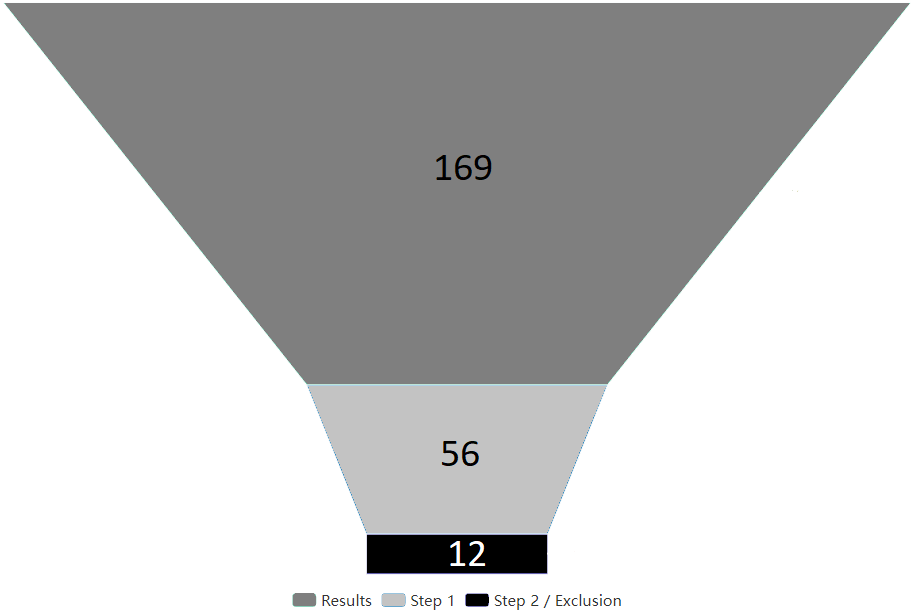
\includegraphics[width=12cm]{img/4-results.png}
  \end{center}
  \fonte{Author.}
\end{figure}

\subsection{Data Extraction}\label{sec:gl-data-extraction}

This section explains how the two data extractions from the discovered tools were carried out: one for the feature matrix and the other to collect more details on the key features shared by the tools.

\subsubsection{Feature Matrix}\label{sec:gl-feature-matrix}

It was important to develop a functions matrix among the filtered results after the research was completed in order to apply the quality standards. In this way, the authors were able to understand which features are present most frequently among the evaluated tools. There were determined to be 37 features in total, some of which repeated more frequently than others. The matrix can be seen in \Cref{fig:gl-matrix}.

\begin{figure}[!htb]
  \caption{Feature Matrix}\label{fig:gl-matrix}
  \begin{center}
    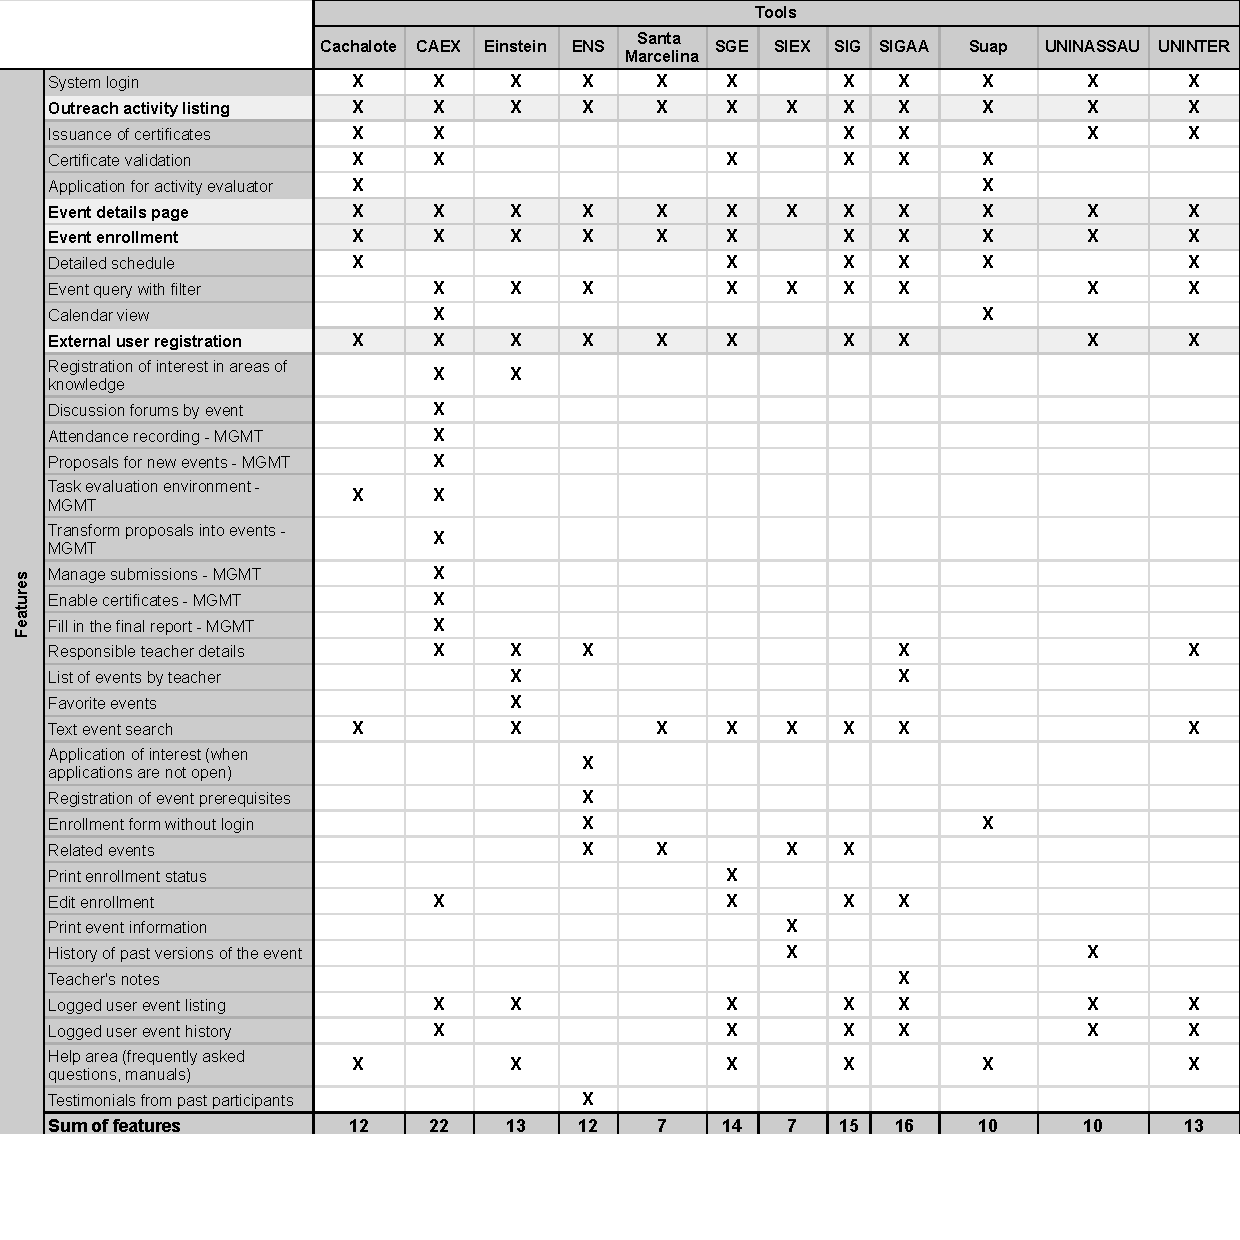
\includegraphics[width=16cm]{img/4-functionality-matrix.pdf}
  \end{center}
  \fonte{Author.}
\end{figure}

Lighter gray highlights were utilized to draw attention to the characteristics that were shared by all of the examined tools and websites so that they could be used as criteria in the subsequent stage of data extraction.

\subsubsection{More Information from Important Features}\label{sec:gl-data-extraction-2}

The goal of the second data extraction was to determine which data was utilized to 
\begin{inparaenum}[(i)]
  \item Listing of outreach activities;
  \item Detailed page of an activity;
  \item Enrollment of a participant into an activity;
  \item Registration of users external to the institution.
\end{inparaenum}

It was challenging to unify the analysis because each tool has its own format and attribute naming, so the original names were kept. To prevent confusion, tools that lacked the chosen features have been highlighted in grey, rather than having the cells left blank. Because it was nearly impossible to try to follow a pattern for all the tools, the extracted findings are written informally. The extracted data can be seen in \Cref{fig:gl-additional-extraction}.

\begin{figure}[!htb]
  \caption{Additional Information Extraction}\label{fig:gl-additional-extraction}
  \begin{center}
    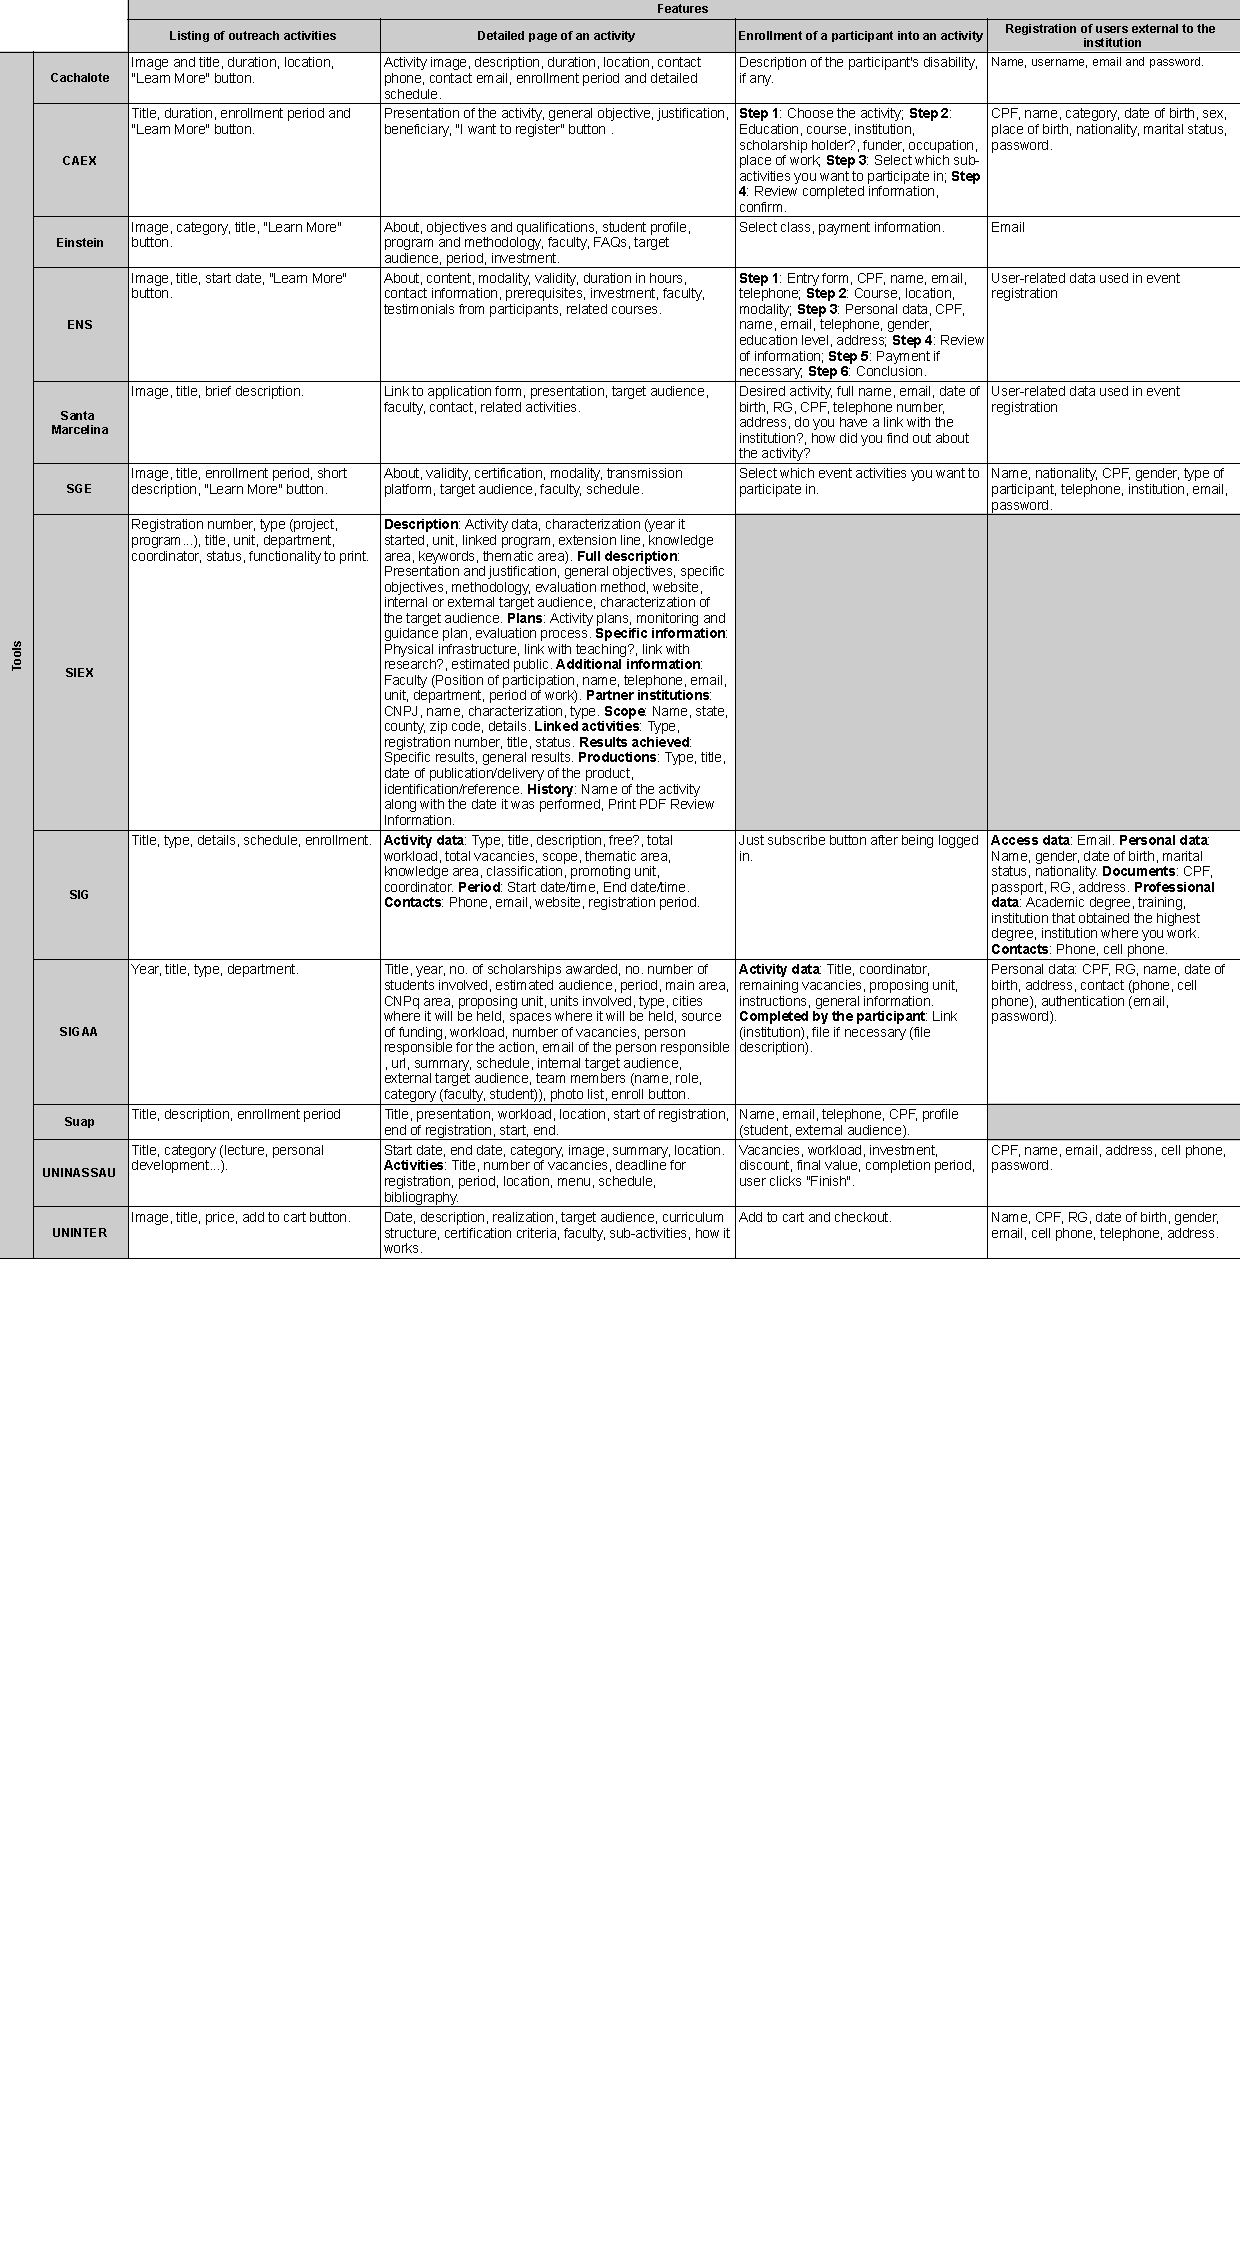
\includegraphics[width=16cm]{img/4-data-extraction-2.pdf}
  \end{center}
  \fonte{Author.}
\end{figure}

\subsection{Tool Classification}\label{sec:gl-tool-classification}

The extracted and tabulated data allowed for the classification of the tools based on the previously established quality standards. The scoring range for a tool is from 0 (zero) to 5 (five). The final results are shown in the table \Cref{tbl:gl-quality-criteria-results}.

\begin{table}[!htb]
  \centering
  \caption{Quality Criteria Evaluation}
  \label{tbl:gl-quality-criteria-results}
  \arrayrulecolor{black}
  \scriptsize
  \begin{tabular}{c|p{2cm}|cc|cc|cc|cc|cc|c}
    \hhline{~~-----------}
    \multicolumn{2}{l}{\multirow{3}{*}{~ ~ ~ ~ ~ ~}}                                & \multicolumn{11}{c}{{\cellcolor[rgb]{0.753,0.753,0.753}}\textbf{Quality Criteria ~ ~ ~ ~ ~ ~ ~ ~}}                                                                                                                                                                                                                                                                                                                                                                                                                                                                                                                                                                                                                                                                                                                                                         \\
    \hhline{~~-----------}
    \multicolumn{2}{l}{}                                                            & \multicolumn{2}{c|}{{\cellcolor[rgb]{0.753,0.753,0.753}}\textbf{QC 1. ~}}                          & \multicolumn{2}{c|}{{\cellcolor[rgb]{0.753,0.753,0.753}}\textbf{QC 2. ~}} & \multicolumn{2}{c|}{{\cellcolor[rgb]{0.753,0.753,0.753}}\textbf{QC 3. ~}} & \multicolumn{2}{c|}{{\cellcolor[rgb]{0.753,0.753,0.753}}\textbf{QC 4. ~}} & \multicolumn{2}{c|}{{\cellcolor[rgb]{0.753,0.753,0.753}}\textbf{QC 5. }} & \multicolumn{1}{l}{{\cellcolor[rgb]{0.753,0.753,0.753}}}                                                                                                                                                                                                                                                                                                                                                                               \\
    \multicolumn{2}{l}{}                                                            & {\cellcolor[rgb]{0.753,0.753,0.753}}\textbf{Ans.}                                                  & {\cellcolor[rgb]{0.753,0.753,0.753}}\textbf{Score}                        & {\cellcolor[rgb]{0.753,0.753,0.753}}\textbf{Ans.}                         & {\cellcolor[rgb]{0.753,0.753,0.753}}\textbf{Score}                        & {\cellcolor[rgb]{0.753,0.753,0.753}}\textbf{Ans.}                        & {\cellcolor[rgb]{0.753,0.753,0.753}}\textbf{Score}       & {\cellcolor[rgb]{0.753,0.753,0.753}}\textbf{Ans.} & {\cellcolor[rgb]{0.753,0.753,0.753}}\textbf{Score} & {\cellcolor[rgb]{0.753,0.753,0.753}}\textbf{Ans.} & {\cellcolor[rgb]{0.753,0.753,0.753}}\textbf{Score} & \multicolumn{1}{l}{\multirow{-2}{*}{{\cellcolor[rgb]{0.753,0.753,0.753}}\begin{tabular}[c]{@{}l@{}}\textbf{Final}\\\textbf{Results }\end{tabular}}}       \\
    \hhline{>{\arrayrulecolor[rgb]{0.753,0.753,0.753}}-->{\arrayrulecolor{black}}-----------}
    \rowcolor[rgb]{0.898,0.898,0.898} {\cellcolor[rgb]{0.753,0.753,0.753}}          & {\cellcolor[rgb]{0.753,0.753,0.753}}\textbf{Cachalote}                                             & 9                                                                         & 0,0                                                                       & No                                                                        & 0,0                                                                      & 12                                                       & 0,5                                               & Partially                                          & 0,5                                               & 2021                                               & 0,5                                                                                                                                                 & 1,5 \\
    {\cellcolor[rgb]{0.753,0.753,0.753}}                                            & {\cellcolor[rgb]{0.753,0.753,0.753}}\textbf{CAEX}                                                  & 4                                                                         & 0,0                                                                       & 7                                                                         & 1,0                                                                      & 22                                                       & 1,0                                               & Yes                                                & 1,0                                               & 2022                                               & 1,0                                                                                                                                                 & 4,0 \\
    \rowcolor[rgb]{0.898,0.898,0.898} {\cellcolor[rgb]{0.753,0.753,0.753}}          & {\cellcolor[rgb]{0.753,0.753,0.753}}\textbf{Einstein}                                              & 12                                                                        & 0,5                                                                       & 1                                                                         & 0,5                                                                      & 13                                                       & 0,5                                               & Partially                                          & 0,5                                               & 2022                                               & 1,0                                                                                                                                                 & 3,0 \\
    {\cellcolor[rgb]{0.753,0.753,0.753}}                                            & {\cellcolor[rgb]{0.753,0.753,0.753}}\textbf{ENS}                                                   & 11                                                                        & 0,5                                                                       & 3                                                                         & 1,0                                                                      & 12                                                       & 0,5                                               & Partially                                          & 0,5                                               & 2022                                               & 1,0                                                                                                                                                 & 3,5 \\
    \rowcolor[rgb]{0.898,0.898,0.898} {\cellcolor[rgb]{0.753,0.753,0.753}}          & {\cellcolor[rgb]{0.753,0.753,0.753}}\textbf{Santa Marcelina}                                       & 6                                                                         & 0,0                                                                       & No                                                                        & 0,0                                                                      & 7                                                        & 0,0                                               & Partially                                          & 0,5                                               & 2022                                               & 1,0                                                                                                                                                 & 1,5 \\
    {\cellcolor[rgb]{0.753,0.753,0.753}}                                            & {\cellcolor[rgb]{0.753,0.753,0.753}}\textbf{SGE}                                                   & 8                                                                         & 0,0                                                                       & 1                                                                         & 0,5                                                                      & 14                                                       & 1,0                                               & Yes                                                & 1,0                                               & 2016                                               & 0,0                                                                                                                                                 & 2,5 \\
    \rowcolor[rgb]{0.898,0.898,0.898} {\cellcolor[rgb]{0.753,0.753,0.753}}          & {\cellcolor[rgb]{0.753,0.753,0.753}}\textbf{SIEX}                                                  & 53                                                                        & 1,0                                                                       & 1                                                                         & 0,5                                                                      & 7                                                        & 0,0                                               & Yes                                                & 1,0                                               & 2022                                               & 1,0                                                                                                                                                 & 3,5 \\
    {\cellcolor[rgb]{0.753,0.753,0.753}}                                            & {\cellcolor[rgb]{0.753,0.753,0.753}}\textbf{SIG}                                                   & 18                                                                        & 0,5                                                                       & No                                                                        & 0,0                                                                      & 15                                                       & 1,0                                               & Partially                                          & 0,5                                               & 2022                                               & 1,0                                                                                                                                                 & 3,0 \\
    \rowcolor[rgb]{0.898,0.898,0.898} {\cellcolor[rgb]{0.753,0.753,0.753}}          & {\cellcolor[rgb]{0.753,0.753,0.753}}\textbf{SIGAA}                                                 & 28                                                                        & 1,0                                                                       & 1                                                                         & 0,5                                                                      & 16                                                       & 1,0                                               & Yes                                                & 1,0                                               & 2022                                               & 1,0                                                                                                                                                 & 4,5 \\
    {\cellcolor[rgb]{0.753,0.753,0.753}}                                            & {\cellcolor[rgb]{0.753,0.753,0.753}}\textbf{Suap}                                                  & 8                                                                         & 0,0                                                                       & No                                                                        & 0,0                                                                      & 10                                                       & 0,5                                               & Yes                                                & 1,0                                               & 2022                                               & 1,0                                                                                                                                                 & 2,5 \\
    \rowcolor[rgb]{0.898,0.898,0.898} {\cellcolor[rgb]{0.753,0.753,0.753}}          & {\cellcolor[rgb]{0.753,0.753,0.753}}\textbf{UNINASSAU}                                             & 14                                                                        & 0,5                                                                       & No                                                                        & 0,0                                                                      & 10                                                       & 0,5                                               & Partially                                          & 0,5                                               & 2022                                               & 1,0                                                                                                                                                 & 2,5 \\
    \multirow{-12}{*}{{\cellcolor[rgb]{0.753,0.753,0.753}}\rotcell{\textbf{Tools}}} & {\cellcolor[rgb]{0.753,0.753,0.753}}\textbf{UNINTER}                                               & 9                                                                         & 0,0                                                                       & No                                                                        & 0,0                                                                      & 13                                                       & 0,5                                               & Partially                                          & 0,5                                               & 2022                                               & 1,0                                                                                                                                                 & 2,0 \\
    \toprule
  \end{tabular}

  \fonte{Author.}
\end{table}

With this classification, it is clear that the \ac{CAEX} tool and \ac{SIGAA} received the highest ratings, which was exactly what was anticipated. First, \ac{SIGAA} is one of the academic management tools that institutions in the nation utilize the most, and \ac{CAEX} is the tool that offered the most distinctive features. As a result, they were two instruments that had a lot of promise and were very helpful in gathering data to create the goal product.

\subsection{Answering the Research Questions}\label{sec:gl-answer-research-questions}

The research questions are under \Cref{tab:research-questions} and were introduced earlier in the study. However, each question is also described below, for the sake of convenience.

\begin{itemize}
  \item \textbf{RQ 1.} What tools currently exist that perform academic management?

        This is a question that also refers to some instruments that were eliminated during the use of inclusion and exclusion criteria. In this instance, 36 tools supporting academic management of various kinds were found, but only 12 of them meet the required requirements and are mentioned in the tool matrix in \Cref{fig:gl-matrix}.
  \item \textbf{RQ 1.1.} Which ones have related functionality or support outreach activities?

        The following tools were found, as it was already demonstrated in \Cref{fig:gl-matrix}, which describes the relationships between tools and features:
        \begin{inparaenum}[(1)]
          \item Cachalote;
          \item CAEX;
          \item Einstein;
          \item ENS;
          \item Santa Marcelina;
          \item SGE;
          \item SIEX;
          \item SIG;
          \item SIGAA;
          \item SUAP;
          \item UNINASSAU and
          \item UNINTER.
        \end{inparaenum}

  \item \textbf{RQ 1.2.} What are the features offered by these tools?

        The features matrix, which is present in \Cref{fig:gl-matrix} and has a total of 37 features, contains a list of every feature that was discovered.
  \item \textbf{RQ 1.3.} What are the most common features between this type of tool?

        The most common functionalities in this type of tool are:
        \begin{inparaenum}[(i)]
          \item A login system;
          \item Lististing of \aclp{OA};
          \item \ac{OA} details page;
          \item \ac{OA} enrollment and
          \item Registration of external users.
        \end{inparaenum}
        The ability to search for events by text is another feature that is present regularly but not as frequently as the other features; 8 of the tools were found to support this functionality.
  \item \textbf{RQ 1.4.} What data do the tools use in relation to activities, participant registration and user registration?

        By analyzing the second data extraction presented in \Cref{sec:gl-data-extraction-2}, the most common fields for \acp{OA} are:
        \begin{inparaenum}[(a)]
          \item Title;
          \item Duration;
          \item Enrollment period;
          \item Contact information;
          \item Description;
          \item Target audience;
          \item Faculty and
          \item Schedule.
        \end{inparaenum}

        Regarding enrollment, the most common fields found are:
        \begin{inparaenum}[(a)]
          \item Participant's personal data;
          \item Institutional affiliation;
          \item Participant type and
          \item Information about the participant's disability, if any.
        \end{inparaenum}

        When it comes to user registration, these tools mostly employ personal information, authentication information, and an address; however, some also request information about the institution, participant type, and professional data.
\end{itemize}

\section{Validity}\label{sec:gl-validity}

Some validity threats were found as the systematic review mapping process progressed. Most of them the authors were able to minimize, but others remain unresolved. They are as follows:

\begin{itemize}
  \item When comparing the findings they both found throughout the study phase, the authors observed that the search results varied just little, between one or two different records. It was an easy threat to mitigate, but it couldn't be completely ruled out. It was decided to perform the search in anonymous mode and log out of the account that was logged into the browser. As a result, there were fewer divergences overall, though there were still some instances of inconsistent outcomes.
  \item Functionalities of the tools weren't checked with the creators. Unfortunately, the authors were unable to reach any universities to ask about the management strategy being employed.
  \item The authors aimed to conduct the search in as little time as possible, beginning and finishing it in just three days, in order to reduce the divergence of findings. As the search engine is regarded as a ``black box'', making it challenging to predict the precise results that will emerge with each search string, the longer the delay, there would be an increasing opportunity to bring threats to the study.
\end{itemize}

\section{Considerations}\label{sec:gl-considerations}

Through this systematic review of the grey literature, it was possible to find tools similar to what the goal product of the whole study should be. Before conducting the review, there was no idea of the current state of the area and of which solutions are most widely used by Brazilian \ac{HEI}.

AA lot of valuable data was gathered regarding the instruments used today. The management and processes for \aclp{OA} were now much more clearly defined. This information will be useful when putting the objective product into use, which seeks to provide a comprehensive solution for \ac{OA} management.

Additionally, it was possible to provide answers to every research question that had been previously stated in the review protocol.         % 27/07
%==============================================================================
\chapter{SURVEY}\label{sec:5}
%==============================================================================

%==============================================================================
Neste capítulo informações mais detalhadas são apresentadas sobre o levantamento (\textit{survey}) que foi conduzido. 
Na \Cref{sec:survey-protocol}, é apresentado detalhes sobre o protocolo adotado, autor de referencia e divisão de tarefas entre os pesquisadores. 
Logo na \Cref{sec:survey-threats}, as ameaças a validade do estudo são relatadas, e por fim na \Cref{sec:survey-results}, todos os resultados alcançados durante a execução são discorridos.

%==============================================================================

\section{Survey Protocol} \label{sec:survey-protocol}

%==============================================================================
Um levantamento (\textit{survey}) é uma abordagem de coleta e análise de dados em que os participantes respondem a perguntas ou a declarações que foram desenvolvidas antecipadamente. 
O protocolo escolhido para a elaboração desta pesquisa foi inspirado nas diretrizes propostas por \citeonline{kasunic2005designing}, em \textit{Designing an effective survey} e está ilustrado na \Cref{fig:setepassos}.

%==============================================================================

\begin{figure}[htb]
  \caption{Seven steps of the research process}\label{fig:setepassos}
  \begin{center}
    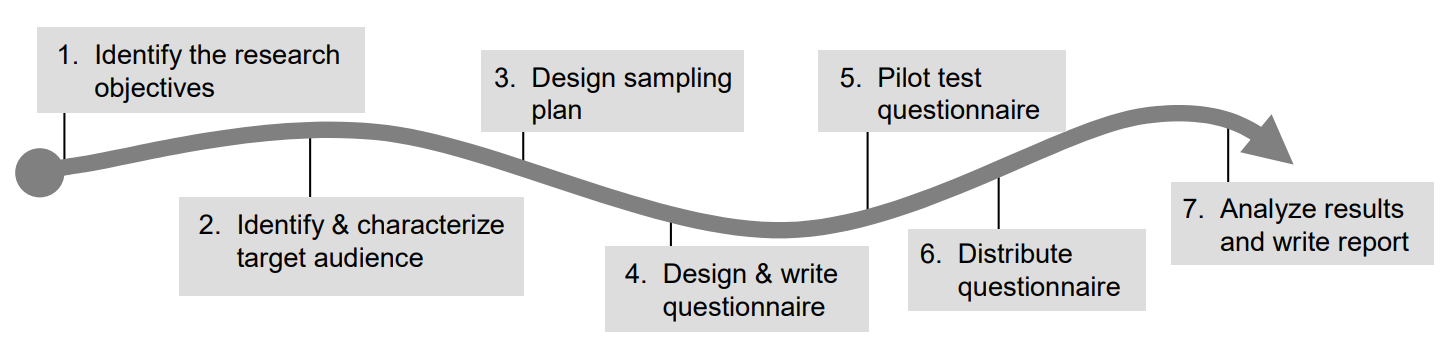
\includegraphics[width=16cm]{img/kasunic_process.png}
  \end{center}
  \fonte{\cite{kasunic2005designing}.}
\end{figure}

%==============================================================================
Como será dito posteriormente, o objetivo é compreender as necessidades de discentes e docentes em relação aos projetos e atividades de extensão. 
A escolha do \textit{survey} como abordagem de coleta de dados se deve ao fato de que as características de uma pesquisa deste tipo nos permite generalizar sobre as crenças e opiniões de muitas pessoas estudando apenas um subconjunto delas \cite{kasunic2005designing}. 
Sendo, neste caso, a ferramenta ideal.

%==============================================================================

%==============================================================================
Tendo em vista que esta pesquisa foi executada por dois estudantes, a carga de trabalho foi dividida, de maneira que a qualidade e desempenho fossem melhorados. 
Na \Cref{tbl:survey-tasks} se encontra a divisão de atividades adotada, contemplando as já definidas por \citeonline{kasunic2005designing}.

%==============================================================================

% Tabela \Cref{tbl:survey-tasks} Activity Division
\begin{table}[!htb]
  \centering
  \caption{Tasks Separation}
  \label{tbl:survey-tasks}
  \footnotesize
  \begin{tabular}{l|l}
    \bottomrule
    \rowcolor[rgb]{0.753,0.753,0.753} \multicolumn{1}{c|}{\textbf{Activity}}                             & \multicolumn{1}{c}{\textbf{Responsibility}} \\
    \hline
    \rowcolor[rgb]{0.898,0.898,0.898} Define and document research objectives                            & Lucas F.                                    \\
    Define and document research questions                                                               & Lucas F.                                    \\
    \rowcolor[rgb]{0.898,0.898,0.898} Define and document how research results will be used              & Lucas F.                                    \\
    Define the appropriate target audience for the research                                              & Igor C.                                     \\
    \rowcolor[rgb]{0.898,0.898,0.898} Determine the appropriate media to apply the research in           & Igor C.                                     \\
    Recruit members of the target audience to participate in pilot test                                  & Igor C.                                     \\
    \rowcolor[rgb]{0.898,0.898,0.898} Breakdown research questions into questionnaire topics             & Lucas F.                                    \\
    Organize and sequence questions                                                                      & Lucas F.                                    \\
    \rowcolor[rgb]{0.898,0.898,0.898} Review the questionnaire based on the pilot test                   & Igor C. and Lucas F.                        \\
    Perform the pilot test                                                                               & Igor C. and Lucas F.                        \\
    \rowcolor[rgb]{0.898,0.898,0.898} Evaluate comments                                                  & Igor C. and Lucas F.                        \\
    Perform final corrections before the distribution of the questionnaire                               & Lucas F.                                    \\
    \rowcolor[rgb]{0.753,0.753,0.753} \multicolumn{1}{c|}{\textbf{Questionnaire ready for distribution}} &                                             \\
    Distribute questionnaires                                                                            & Lucas F.                                    \\
    \rowcolor[rgb]{0.898,0.898,0.898} Monitor answers                                                    & Igor C. and Lucas F.                        \\
    Send reminders                                                                                       & Igor C.                                     \\
    \rowcolor[rgb]{0.753,0.753,0.753} \multicolumn{1}{c|}{\textbf{Questionnaire response deadline}}      &                                             \\
    Perform analysis                                                                                     & Igor C. and Lucas F.                        \\
    \rowcolor[rgb]{0.898,0.898,0.898} Write draft report                                                 & Igor C.                                     \\
    Revise draft                                                                                         & Igor C. and Lucas F.                        \\
    \rowcolor[rgb]{0.898,0.898,0.898} Perform the final corrections                                      & Igor C. and Lucas F.                        \\
    \toprule
  \end{tabular}
\end{table}

\subsection{Identify the Research Objectives} \label{sec:survey-objectives}
% Objetivo do survey -> refinamento dos requisitos, validar, importancia
% Transformar em uma questão de pesquisa, pergunta
% grey gerou resultados pra usar no survey com o olhar dos futuros usuarios

%==============================================================================
O objetivo deste primeiro passo é identificar qual a importância e o por que de fazer um survey, o que poderia ser conquistado com ele.
Levando em conta os resultados gerados pela revisão na literatura cinza, mencionados no \Cref{grey_literature}, foi possível elaborar questões de maneira que o participante informe, na sua visão, a importância de determinado requisito levantado. 
Logo, o objetivo deste survey é ordená-los por prioridade, utilizando a opinião de possíveis usuários finais.
%==============================================================================

%==============================================================================
Além de ser perguntado a opinião dos participantes, foi permitido com que eles fornecessem sugestões ou melhorias em relação a requisitos da ferramenta, já que um dos objetivos da pesquisa está voltado a entender as necessidades dos possíveis usuários do sistema. 
Assim, tendo uma base mais sólida para começar o processo de desenvolvimento da solução corretamente, com os escopos das atividades mais bem definidos.

%==============================================================================
\subsection{Identify and Characterize the Target Audience} \label{sec:survey-targets}
%==============================================================================
Neste estágio, é necessário olhar para os possíveis públicos respondentes e identificar quem será o público respondente e quem é a população do estudo. Assim sendo, a população é composta por todos as pessoas dentro da comunidade acadêmica, logo foi escolhido para representarem a amostra desta população os coordenadores de programas ou projetos de extensão, docentes e discentes, tendo preferência em participantes que tenham experiência com atividades de extensão. Com este público é possível ter o ponto de vista de todos os usuários da ferramenta, quem cria atividades e quem se inscreve em uma.
%==============================================================================
% Para possívelmente conseguir melhores sugestões nas respostas do survey, foi necessário abrangir a maior quantidade de campus da \ac{UNIPAMPA} possivel, era esperado que campus como Uruguaiana, Bagé e Dom Pedrito que, como visto na \Cref{fig:number-of-projects} foram os campus que mais possuiram atividades de extensão no ano de 2017 de acordo com \cite{relatorio-2017}, fornecessem mais respondentes, mas no final isto nao aconteceu.

% \begin{figure}[htb]
%   \caption{Number of Projects Contemplated in the Internal Public Notices}\label{fig:number-of-projects}
%   \begin{center}
%     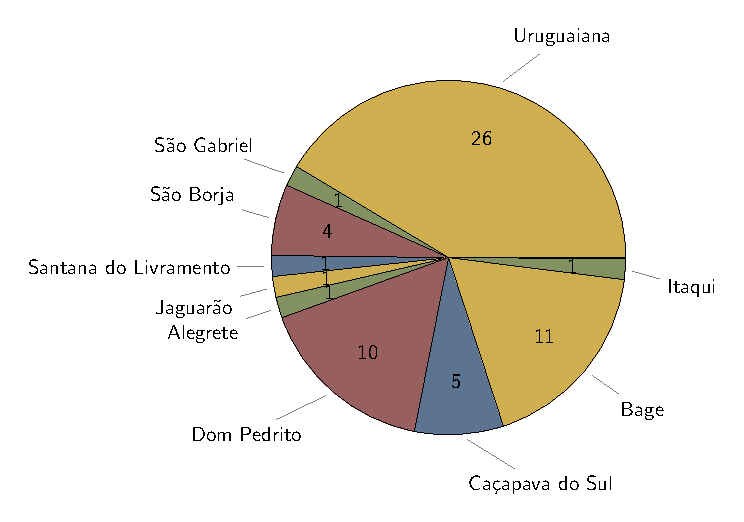
\includegraphics[width=16cm]{img/uruguaiana.pdf}
%   \end{center}
%   \fonte{Adapted from \cite{relatorio-2017}}
% \end{figure}

\subsection{Design the Sampling Plan} \label{sec:survey-sampling}

%==============================================================================
De acordo com \citeonline{kasunic2005designing}, o objetivo desta fase é determinar os seguintes tópicos:
\begin{itemize}
    \item How individuals will be selected to participate in the survey;
    \item The required size of the sample.
\end{itemize}
%==============================================================================

%==============================================================================
Por isso, o primeiro tópico buscou abrangir a maioria de campus da \ac{UNIPAMPA} possível por meio de envio de emails para as suas secretarias academicas, direcionados para os alunos e para listas de coordenadores de programas e projetos de extensão, mantendo o equilibrio entre docentes e discentes. 
Com isso, campus como Uruguaiana, Bagé e Dom Pedrito que, como visto na \Cref{fig:number-of-projects} foram os campus que mais possuíram atividades de extensão no ano de 2017 \cite{relatorio-2017}, assim, esperava-se que fornecessem mais respondentes para a pesquisa.
%==============================================================================
\begin{figure}[htb]
  \caption{Number of Projects Contemplated in the Internal Public Notices}\label{fig:number-of-projects}
  \begin{center}
    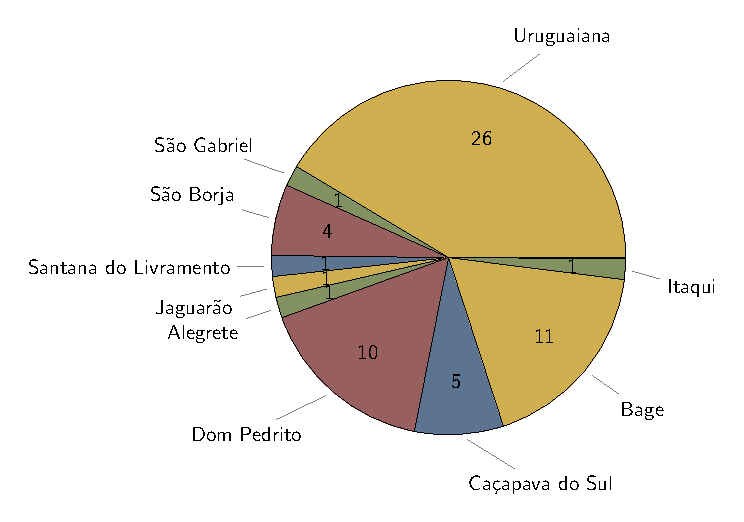
\includegraphics[width=16cm]{img/uruguaiana.pdf}
  \end{center}
  \fonte{Adapted from \cite{relatorio-2017}}
\end{figure}

%==============================================================================
Em relaçao ao tamanho mínimo da amostra, tamanhos entre 100 e 150 respondentes já seriam suficientes, pois além das respostas quantitativas teriam todas as respostas qualitativas com sugestões e melhorias, demandando mais tempo para análise.
%==============================================================================

%==============================================================================
A separação da amostra é um ponto essencial para a melhor eficiência do survey, estando de acordo com a prática recomendada 22 definida por \citeonline{Jefferson}, em que diz que a amostra deve ser dividida de acordo com as suas caracteristicas e semelhanças. 
Para contemplá-la, os respondentes do questionário que se declarassem como \acp{TAE} ou docentes eram direcionados para uma área do questionário, e discentes para outra, ambas as áreas com perguntas relacionadas ao perfil reclarado pelo respondente.

%==============================================================================
\subsection{Design and Write the Questionnaire} \label{sec:survey-questionnaire}

% (kasunic) objetivos e caracteristicas da sample para fazer o questionario, importancia dos dois
% (guideline) resultados dependem da qualidade das perguntas

% (kasunic) 4 tipos de perguntas, colcoar as que se encaixam em cada uma
% (kasunic) close ended e open ended questions 52, todas sao ordinal responses usando MoSCoW

% Colocar o questionario em apendice
%==============================================================================
\citeonline{kasunic2005designing} ressalta que para a estruturação e escrita do questionário, os objetivos de pesquisa e as características da amostra devem ser levados em conta. 
De acordo com o autor, questionarios que não possuem objetivos bem definidos tem mais chances de possuirem perguntas que só consomem tempo do respondente, ele ressalta isso com uma pergunta \citeonline[p.34]{kasunic2005designing} ``How can you reach insightful conclusions if you do not know what you were looking for or planning to observe?'', neste questionário o objetivo é bem definido, focado em priorização de requisitos e levantamento de sugestões pelos possíveis usuários finais como bem descrito na \Cref{sec:survey-objectives}. 
Da mesma maneira, as caracteristicas da amostra são importantes para escrever as perguntas de um modo que todos entendam e não apenas pensando no entendimento dos proprios pesquisadores. 
% \citeonline[p.23]
\citeonline{surveyGuidelines} atenta que os resultados que serão obtidos com o survey, estão diretamente relacionados com a qualidade do questionário utilizado.
%==============================================================================

%==============================================================================
Para \citeonline{surveyGuidelines} existem dois tipos de questionários, self-administrated and interviewer-administrated questionnaire, de acordo com suas definições este se encaixa no primeiro tipo, pois por ser um questionario web-based, não é necessário ao acompanhamento dos pesquisadores. 
Este modelo permite a maior abrangência de respondentes, mas por outro lado tende a maior taxa de desistência, ressaltando a importância de uma boa estruturação.
%==============================================================================

%==============================================================================
Para a realização do survey, foi escolhida a ferramenta do Google Forms, já que ela contribui com uma interface simples e de facil entendimento, logo que esta já é utilizada pela maioria dos perfis dos respondentes.
%==============================================================================

%==============================================================================
A estrutura do questionário que está contido no \Cref{annex:questionnaire} se da pela página inicial, questões de perfil do respondente, questões de priorização de requisitos e por fim sugestões de funcionalidades, estas estão descritas a seguir em suas respectivas seções.
%==============================================================================
\subsubsection{The Welcome Screen}
%==============================================================================
% \citeonline[p.65]
Seguindo instruções de \citeonline{kasunic2005designing}, a primeira página do questionário contém informações importantes para o participante como:

%==============================================================================

%==============================================================================
\begin{itemize}
  \item O objetivo da pesquisa;
  \item Duração estimada do questionário;
  \item Endereços de email para contato;
  \item Pesquisadores envolvidos;
  \item Caráter voluntário, anônimo e confidencial da pesquisa;
  \item Instituição e organização envolvida.
\end{itemize} 
Por fim perguntando para o participante se ele aceita em continuar com a pesquisa.

%==============================================================================

\subsubsection{Profile Questions}\label{survey:profile-questions}
%==============================================================================
As questões referentes a adiquirir informações sobre o participante são importantes nas primeiras fases do questionario, pois motivam os participantes a continuar respondendo-o sem confundi-los com perguntas complexas logo no começo, \cite{LMRea}. Além que com uma boa classificação de participantes, permite que a analise destes seja feita de maneira mais controlada e organizada como bem mencionado por \citeonline{legramante}.
%==============================================================================

%==============================================================================
Os dados que foram retirados com as perguntas de perfil, são listadas a seguir:
\begin{inparaenum}[(1)]
  \item Se o participante faz parte da \ac{UNIPAMPA};
  \item Sexo do participante;
  \item Faixa etária;
  \item Formação acadêmica;
  \item Se o participante ja esteve em alguma atividade extensionista;
  \item Se a anterior for verdadeira, quais papeis ele desempenhou;
  \item Papel do participante na comunidade acadêmica;
  \item Campus/Cidade do participante;
  \item Curso em que esta relacionado.
\end{inparaenum}
%==============================================================================

\subsubsection{Requisites Priorization Questions}
%==============================================================================
Nas perguntas relacionadas ao objetivo da pesquisa foram utilizados alguns direcionamentos descritos por \citeonline{forza}, são eles:
% \citeonline[p.168]
\begin{description}
  \item \textbf{Suggestion 1.} Define the way questions are asked to collect the information on a specific concept;\label{suggestion:1}
  \item \textbf{Suggestion 2.} For each question decide the scale on which the answers are placed;\label{suggestion:2}
  \item \textbf{Suggestion 3.} Identify the appropriate respondent(s) to each question;\label{suggestion:3}
  \item \textbf{Suggestion 4.} Put together the questions in questionnaires that facilitate and motivate the respondent(s) to respond.\label{suggestion:4}
\end{description}
%==============================================================================

%==============================================================================
Em se tratando do \textbf{Suggestion 1}, onde é sugerido que as perguntas estejam escritas de maneira que toda a amostra respondente consiga entender e formular uma resposta. 
Já que as perguntas deste questionario se referem a requisitos de software, foi utilizado o modelo de estórias de usuário, em que deixa bem explícito qual o ator, o que se deseja com o determinado requisito e o seu motivo. 
Também foi determinado que as perguntas seriam classificadas como closed questions, que determinam as possíveis respostas do respondente como descrito por \citeonline{forza}. 
Assim, no final de cada página do questionário também continha uma questão open-ended permitindo o respondente dissertar da maneira que bem entender.
%==============================================================================

%==============================================================================
A \textbf{Suggestion 2} se trata da escala utilizada nas perguntas, em um primeiro momento pensou-se em utilizar a escala Likert, mas melhor pensado posteriormente decidiu-se utilizar a escala \ac{MoSCoW}, sendo as possíveis respostas as já presentes no seu próprio nome. 
Ela foi escolhida porque esta mais relacionada a requisitos e serve justamente para a priorização de requisitos de software.
%==============================================================================

%==============================================================================
Em seguida na \textbf{Suggestion 3}, sugere-se que o questionário direcione os participantes para as perguntas que eles possuam mais propriedade para respondê-las, trazendo respostas mais construtivas e relevantes. 
No questionário utilizado, esta divisão esta sendo feita utilizando as perguntas de perfil comentadas na \Cref{survey:profile-questions}, sendo o participante automaticamente direcionado para a seção correspondente com seu perfil.
%==============================================================================

%==============================================================================
Por fim, na \textbf{Suggestion 4} é aconselhado que todas as perguntas que tem um assunto em comum, sejam organizadas próximas umas das outras para facilitar as verificações cruzadas entre as respostas. 
Para implementar esta sugestão, os requisitos estão agrupados por papéis conforme os atores do sistema, sendo eles: 
\begin{inparaenum}[(1)]
    \item Proponente de atividade de extensão;
    \item Instrutor de atividades de extensão;
    \item Coordenador de projetos ou programas de extensão;
    \item Participante de atividades de extensão.
\end{inparaenum}
%==============================================================================
\subsubsection{Feature Suggestions}
%==============================================================================
Para a última página do questionário foi disponibilizado um campo em que os respondentes podem sugerir aos pesquisadores qualquer melhoria, funcionalidade, correção etc. Com estas respostas é possível fazer uma analise qualitativa e conseguir novas ideias para o desenvolvimento e completude da ferramenta final.
%==============================================================================
\subsection{Pilot Questionnaire}\label{sec:survey-pilot}
%==============================================================================
Após ser gerado uma versão estável do questionario, é necessário validá-lo, para isto foi realizado um questionário piloto. 
% \citeonline[p.75]{kasunic2005designing} 
De acordo com \citeonline{kasunic2005designing} a pilot test is a simulation of the real questionnaire carried out with a small number of members from the target audience. 
Para realizá-lo foram escolhidas 7 (sete) pessoas, divididas em: 4 (quatro) alunos de graduação, 2 (dois) professores da \ac{UNIPAMPA} campus Alegrete e 1 (um) \ac{TAE}. 
A escolha dos respondentes do questionario piloto se deu porque ela representa todos os perfis esperados na target sample, e representa a proporção esperada na realização real do questionario.
%==============================================================================

%==============================================================================
Dos escolhidos para a participação do questionário piloto apenas um não conseguiu respondê-lo a tempo, este foi o \ac{TAE}, mas isto no final não foi um problema pois como mencionado na \Cref{sec:survey-sampling}, o questionário está divido em duas partes em que \acp{TAE} e docentes respondem a mesma.
%==============================================================================

%==============================================================================
Com a execução deste piloto foi possível adiquirir diversas sugestões, correções e pontos importantes para a versão final do questionário. 
Um exemplo disso, foi que um participante não se sentiu confortável expondo a sua idade exata, então foi sugerido que esta fosse solicitada utilizando faixas etárias.
%==============================================================================
\subsection{Distribute the Questionnaire}\label{sec:survey-distribute}

O questionário foi distribuído para todas as pessoas que compõem a amostra desta pesquisa. 
Para isto ser executado, primeiro foi realizado uma pesquisa para levantar todos os emails de coordenadores de projetos ou programas de extensão de todos os campus da \ac{UNIPAMPA}, sendo eles os primeiros a responder as respostas do questionario. 
Após 2 (dois) dias, foi enviado emails para todas as secretarias academicas dos campus, solicitando que fosse repassado para todos os seus alunos de todos os cursos. 
Concluindo, ao todo o survey ficou aberto para respostas por 18 (dezoito) dias.

\subsection{Analyze the Results and Write a Report}\label{sec:survey-analyse}

Os resultados quantitativos relacionados a priorização de requisitos, devem ser coletados e organizados em gráficos para melhor entendimento e visualização dos dados. 
Assim será possível ter uma lista ordenada de requisitos que foram considerados mais importantes para os usuários finais.

Em relação as respostas qualitativas, estas serão analisadas caso a caso e se pertinente a sugestão, serão adicionadas dentro do leque final de funcionalidades ou melhorias.

\section{Threats to Validity}\label{sec:survey-threats}

% Decições, problemas, descrever como tentamos contornar a ocorrencia
% Olhar nos trabalhos para exemplos de ameaças
% Piloto, estruturação...

\section{Result Analysis}\label{sec:survey-results}

\subsection{--} % Separação dos participantes, aluno, professor, idade, campus...

\subsection{--} % Participação em algum projeto de extensão

\subsection{--} % Classificação final, graficos       % 27/07
% Extensionly - análise e projeto de software, artefatos da implementação, maior capítulo de todos, modelo de domínio, diagrama de componentes, paradigma de programação, tecnologias, processo da engenharia de software, separação frontend/backend (com mais detalhes técnicos), usar figuras e modelos
%==============================================================================
\chapter{Extensionly Backend Design}\label{extensionly}
%==============================================================================

% ===================================
% Este capítulo descreve particularidades da ferramenta Extensionly, decisões relacionadas ao backend entre outras decisões de design.

This chapter describes the particularities of the Extensionly tool, decisions related to the backend and other design decisions.
% ===================================

\section{Initial Considerations}\label{sec:ext-considerations}
% ===================================
% A ferramenta Extensionly, por ter como objetivo incorporar e reproduzir todos ou a maioria dos processos envolvendo atividades de extensão, o seu desenvolvimento é divido entre dois alunos estando um responável pelo frontend e outro pelo backend que é o objetivo deste trabalho. 
% Para o desenvolvimento acontecer de forma fluida e performatica, a comunicação entre os desenvolvedores deve ser constante, pois qualquer mudanca em regras de negocio devem estar muito claras por ambas as partes.

The Extensionly tool, as it aims to incorporate and reproduce all or most of the processes involving \acl{OA}, its development is divided between two students, one being responsible for the frontend and the other for the backend, which is the objective of this work.
The project will be versioned utilizing Git, a version control tool designed to efficiently and quickly manage any project, no matter how big or small \cite{chacon2014pro}. The source code will be split between two repositories, one for the frontend\footnote{Extensionly Frontend code is available at \url{https://github.com/Dalepfell/extensionly-frontend}} and one for the backend\footnote{Extensionly Backend code is available at \url{https://github.com/IgorDalepiane/extensionly-backend-service}}.

For development to happen in a fluid and performative way, communication between developers must be constant, as any change in business rules must be very clear by both parties.
% ===================================

% ===================================
% O propósito geral da ferramenta além de suportar variados processos envolvendo extensão universitária, é estreitar as relações entre a comunidade externa e acadêmica, criando um canal de comunicação em que possa ser geradas demandas para a universidade. 
% Sendo assim, os alunos vão estar cada vez mais acostumados e vinculados com a comunidade como um todo, atribuindo muito valor e experiencia a sua formação.

The general purpose of the tool, in addition to supporting various processes involving university outreach, is to strengthen relations between the external and academic community, creating a communication channel in which demands can be generated for the university.
Therefore, students will be increasingly accustomed to and linked to the community as a whole, attributing much value and experience to their formation.
% ===================================

% ===================================
% A ferramenta tem como primeiro objetivo ser utilizada pela unipampa campus alegrete, mas não dispensando possiveis expansões futuras, para todos os campus da instituição e até mesmo para outras instituições do Brasil. 
% Para isto a implementação deve ser realizada de uma maneira que seja diminuido o custo quando estas novas decisões de projeto forem tomadas.

The first objective of the tool is to be used by \ac{UNIPAMPA} Campus Alegrete, but not dispensing with possible future expansions, for all the institution's campuses and even for other institutions in Brazil.
For this the implementation must be carried out in a way that the cost is reduced when these new design decisions are made.
% ===================================
% Ferramenta Desenvolvida em conjunto
% Comunicação entre os dois
% Proposito da ferramenta é estreitar as relações entre a comunidade, alunos estrem mais vinculados com a comunidade como um todo,
% Objetivo de fazer um teste piloto em 2023 janeiro
% Primeiro case da ferramenta é a Unipampa, mas ja pensando em possiveis expansoes para todas as instituições

\section{Extensionly Requirements}\label{sec:ext-req}
% ===================================
% Esta seção esta direcionada a apresentar em mais detalhes os requisitos funcionais levantados pelo estudo, o qual foi divido em duas partes principais, primeiro sendo conduzida uma revisão na literatura cinza, como apresentado na \Cref{grey_literature}, e depois com os resultados analisados e transformados em estorias de usuario, foi aplicado o survey descrito na \Cref{sec:5} 
This section is intended to present in more detail the functional requirements raised by the study, which was divided into two main parts, first being conducted a review of the gray literature, as presented in \Cref{grey_literature}, and then, with the results analyzed and transformed into user stories, they were applied to the survey described in \Cref{sec:5}

% ===================================

\subsection{Requirements Obtained through the Grey Literature Review}\label{req-grey}
% ===================================
% Na execução da revisão da literatura cinza, analisando outras ferramentas similares, como ja bem descrito na \Cref{grey_literature}, foram levantados algumas funcionalidades presentes nas ferramentas como mostra a \Cref{sec:gl-feature-matrix}, dentre eles 28 (twenty eight) \acp{FR} foram selecionados para participarem da proxima fase, o survey. 
% Então os desenvolvedores junto com seu supervisor, analisaram caso a caso e classificaram a sua prioridade entre:
% \begin{inparaenum}[(1)]
% \item High 
% \item Medium 
% \item Low 
% \end{inparaenum}.
% Alguns destes requisitos foram removidos após a classificação, pois eram muito complexos para o contexto de um \ac{MVP}, ou não faziam parte de escopo simplesmente.

In carrying out the review of the gray literature, analyzing other similar tools, as already described in \Cref{grey_literature}, some functionalities present in the tools were raised, as shown in \Cref{sec:gl-feature-matrix}, among them 28 (twenty eight) \acp{FR} were selected to participate in the next phase, the survey.
So the developers, together with their supervisor, analyzed it on a case-by-case basis and ranked their priority among:
\begin{inparaenum}[(1)]
    \item High;
    \item Medium;
    \item Low.
\end{inparaenum}
Some of these requirements were removed after classification, as they were too complex for the context of an \ac{MVP}, or simply not in scope. All the initial requirements among with their priority can be found in \Cref{tab:initial-requirements}.
% ===================================

\begin{table}[!htb]
  \centering
  \setlength{\aboverulesep}{0pt}
  \setlength{\belowrulesep}{0pt}
  \caption{Initial Requirements}
  \label{tab:initial-requirements}
  \footnotesize
  \begin{tabular}{c|l|c}
    \toprule
    \rowcolor[rgb]{0.753,0.753,0.753} \textbf{ID} & \multicolumn{1}{c|}{\textbf{Requirement}}                    & \textbf{Priority} \\
    \hline
    \rowcolor[rgb]{0.898,0.898,0.898} FR. 01      & Propose new OAs                                              & High              \\
    FR. 02                                        & Allow enrollments in OA                                      & High              \\
    \rowcolor[rgb]{0.898,0.898,0.898} FR. 03      & Record participant attendance                                & High              \\
    FR. 04                                        & Review and approve OA proposals                              & High              \\
    \rowcolor[rgb]{0.898,0.898,0.898} FR. 05      & Text search for OAs                                          & High              \\
    FR. 06                                        & Registration of OA prerequisites                             & High              \\
    \rowcolor[rgb]{0.898,0.898,0.898} FR. 07      & Edit enrollment status in OAs                                & High              \\
    FR. 08                                        & List OAs the user is enrolled in                             & High              \\
    \rowcolor[rgb]{0.898,0.898,0.898} FR. 09      & Maintain history of OAs participated                         & High              \\
    FR. 10                                        & Help area (frequently asked questions, manuals)              & High              \\
    \rowcolor[rgb]{0.898,0.898,0.898} FR. 11      & OAs query with filter                                        & Medium            \\
    FR. 12                                        & External user registration                                   & Medium            \\
    \rowcolor[rgb]{0.898,0.898,0.898} FR. 13      & Registration of interest in areas of knowledge               & Medium            \\
    FR. 14                                        & Show proponent details                                       & Medium            \\
    \rowcolor[rgb]{0.898,0.898,0.898} FR. 15      & Favorites list for OAs                                       & Medium            \\
    FR. 16                                        & Declare interest in an OA (when enrollments are not open)    & Medium            \\
    \rowcolor[rgb]{0.898,0.898,0.898} FR. 17      & Share OA information                                         & Medium            \\
    FR. 18                                        & OA past versions history                                     & Medium            \\
    \rowcolor[rgb]{0.898,0.898,0.898} FR. 19      & Teacher's note in the OA details                             & Medium            \\
    FR. 20                                        & Final OA assessment by the student                           & Medium            \\
    \rowcolor[rgb]{0.898,0.898,0.898} FR. 21      & Detailed schedule for upcoming OAs                           & Low               \\
    FR. 22                                        & Fill in final OA report~                                     & Low               \\
    \rowcolor[rgb]{0.898,0.898,0.898} FR. 23      & Print enrollment status                                      & Removed           \\
    FR. 24                                        & Testimonies/reviews from past participants in the OA details & Removed           \\
    \rowcolor[rgb]{0.898,0.898,0.898} FR. 25      & Instructor/student communication channel                     & Removed           \\
    FR. 26                                        & Environment for evaluation of students submitted works       & Removed           \\
    \rowcolor[rgb]{0.898,0.898,0.898} FR. 27      & List of OAs by teacher                                       & Removed           \\
    FR. 28                                        & List of related OAs                                          & Removed           \\
    \bottomrule
  \end{tabular}
\end{table}

The following are sketches of how the initial requirements relate to the defined user roles. \Cref{fig:use-case-1} presents the first 14 \ac{FR} and \Cref{fig:use-case-2}, the remaining 8, excluding the ones that were removed.

\begin{figure}[!htb]
  \caption{User Roles on the First 14 \ac{FR}}\label{fig:use-case-1}
  \begin{center}
    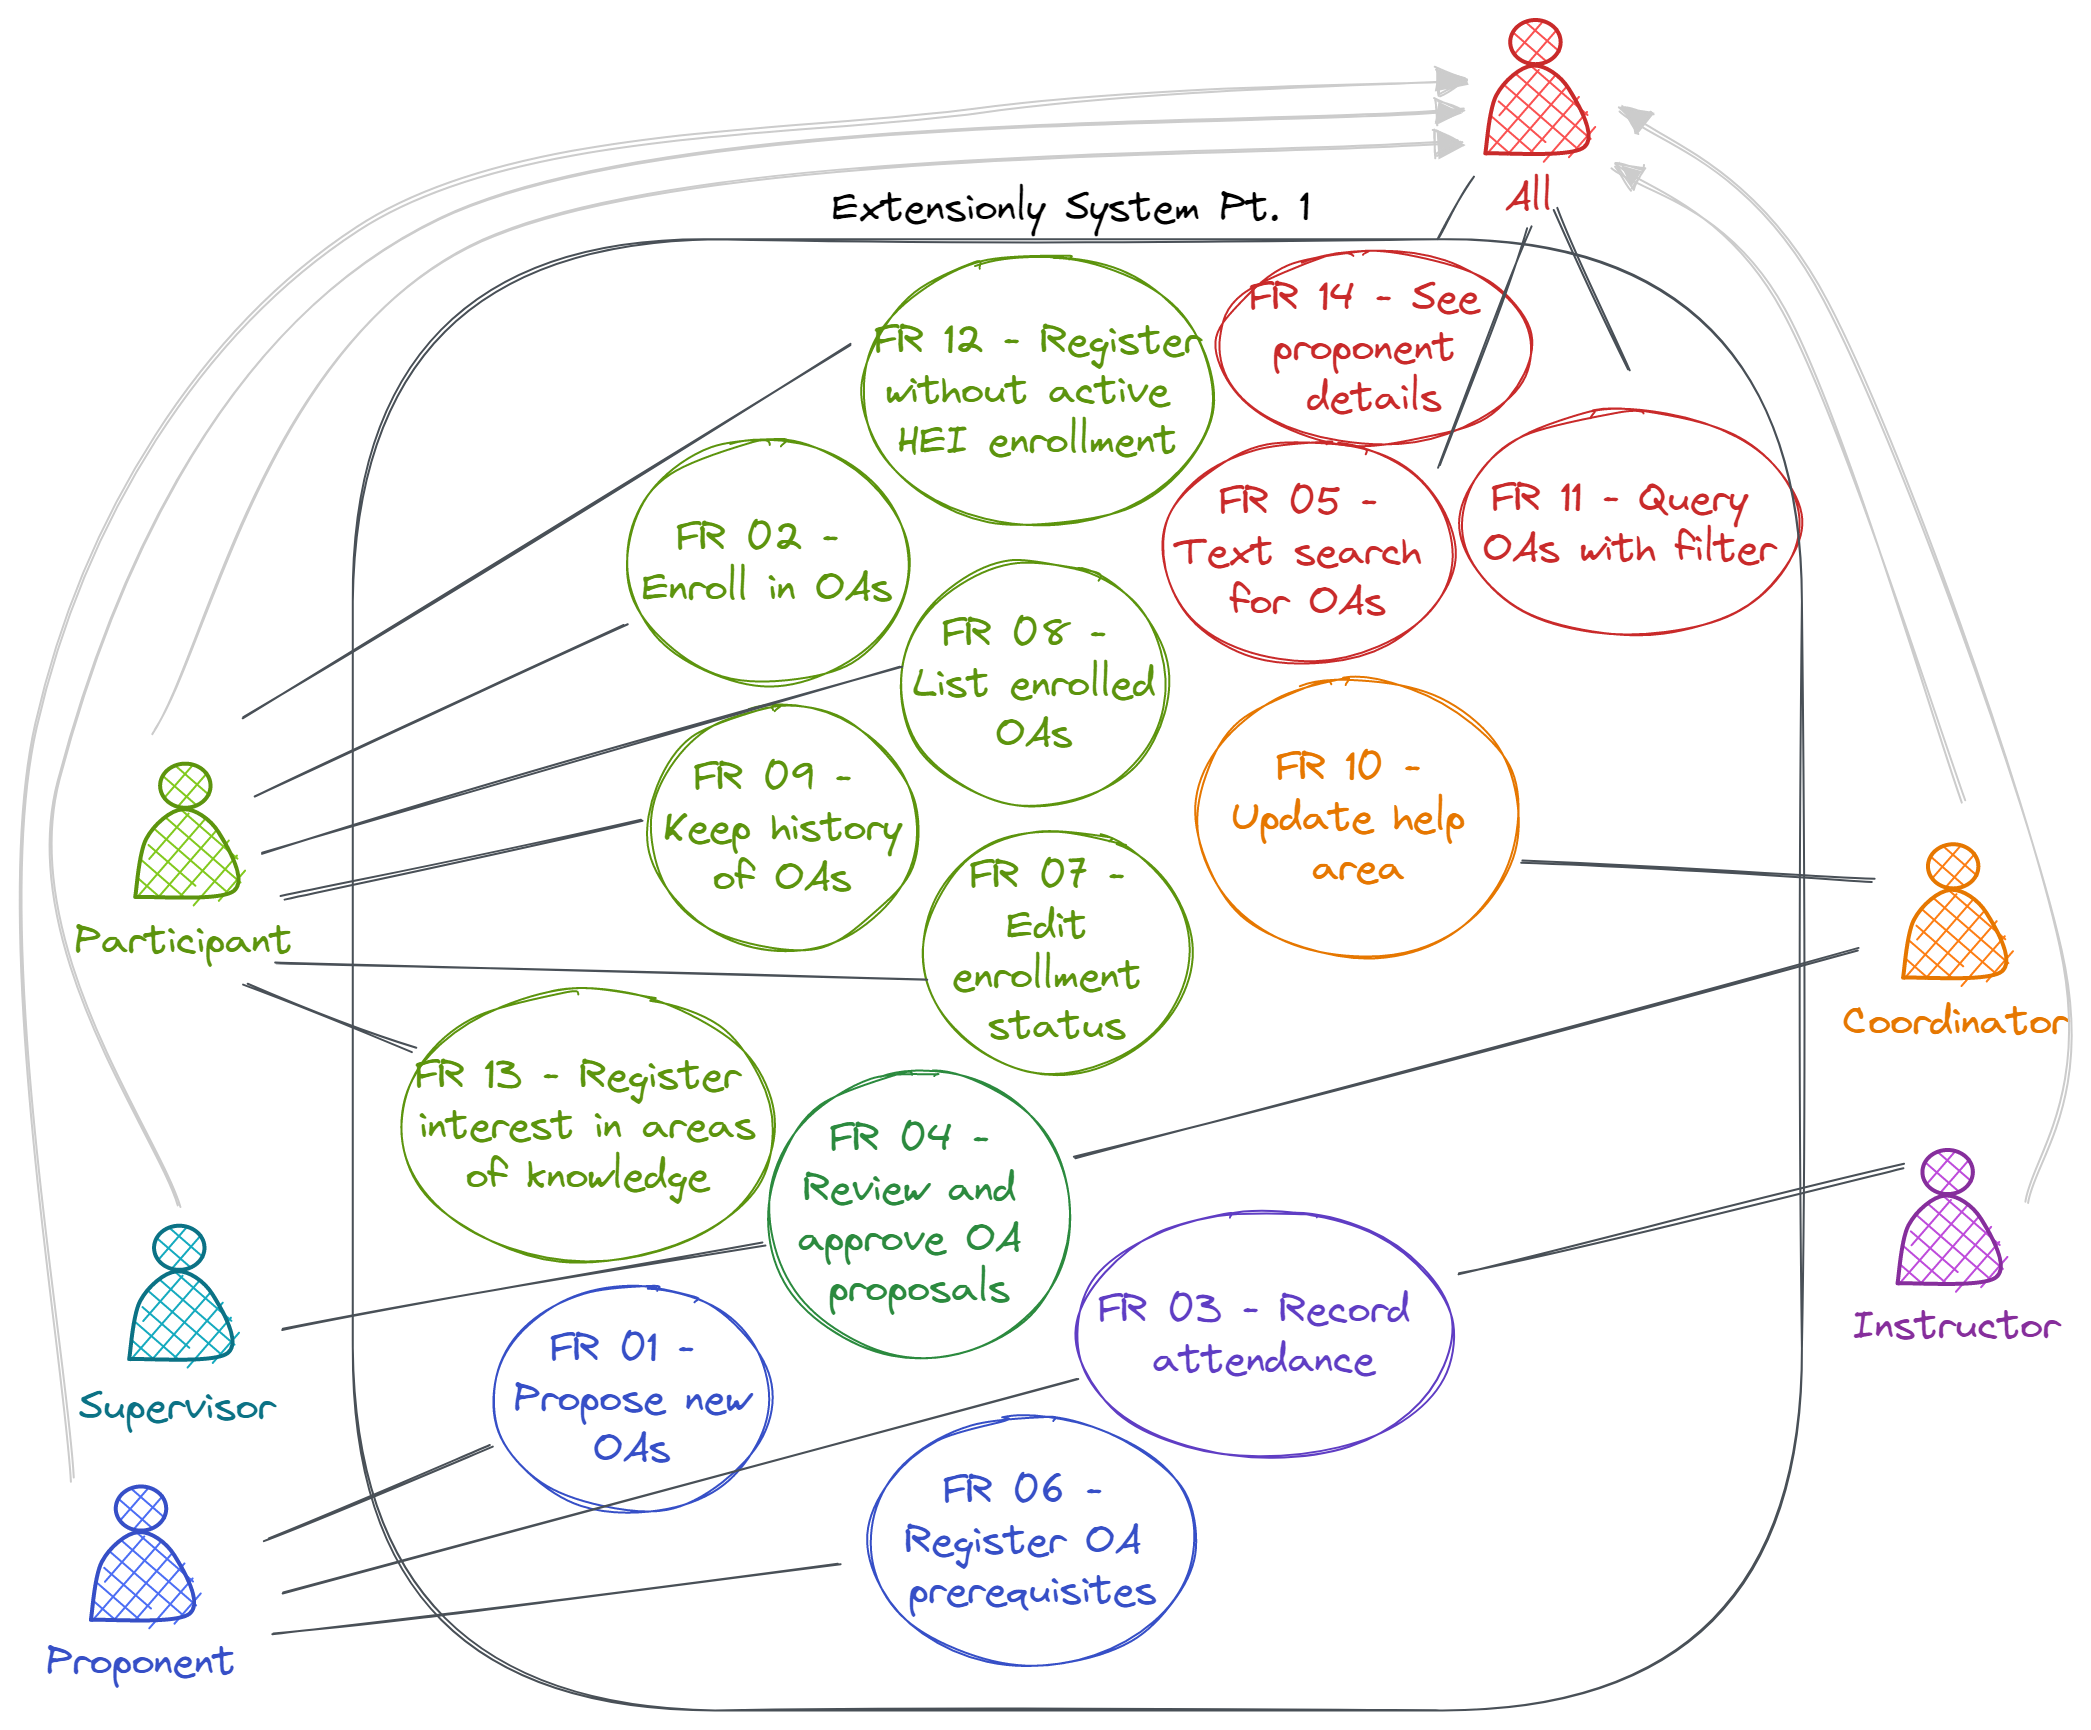
\includegraphics[width=15cm]{img/6-use-case-1.png}
  \end{center}
  \fonte{Author.}
\end{figure}

\begin{figure}[!htb]
  \caption{User Roles on the Last 8 \ac{FR}}\label{fig:use-case-2}
  \begin{center}
    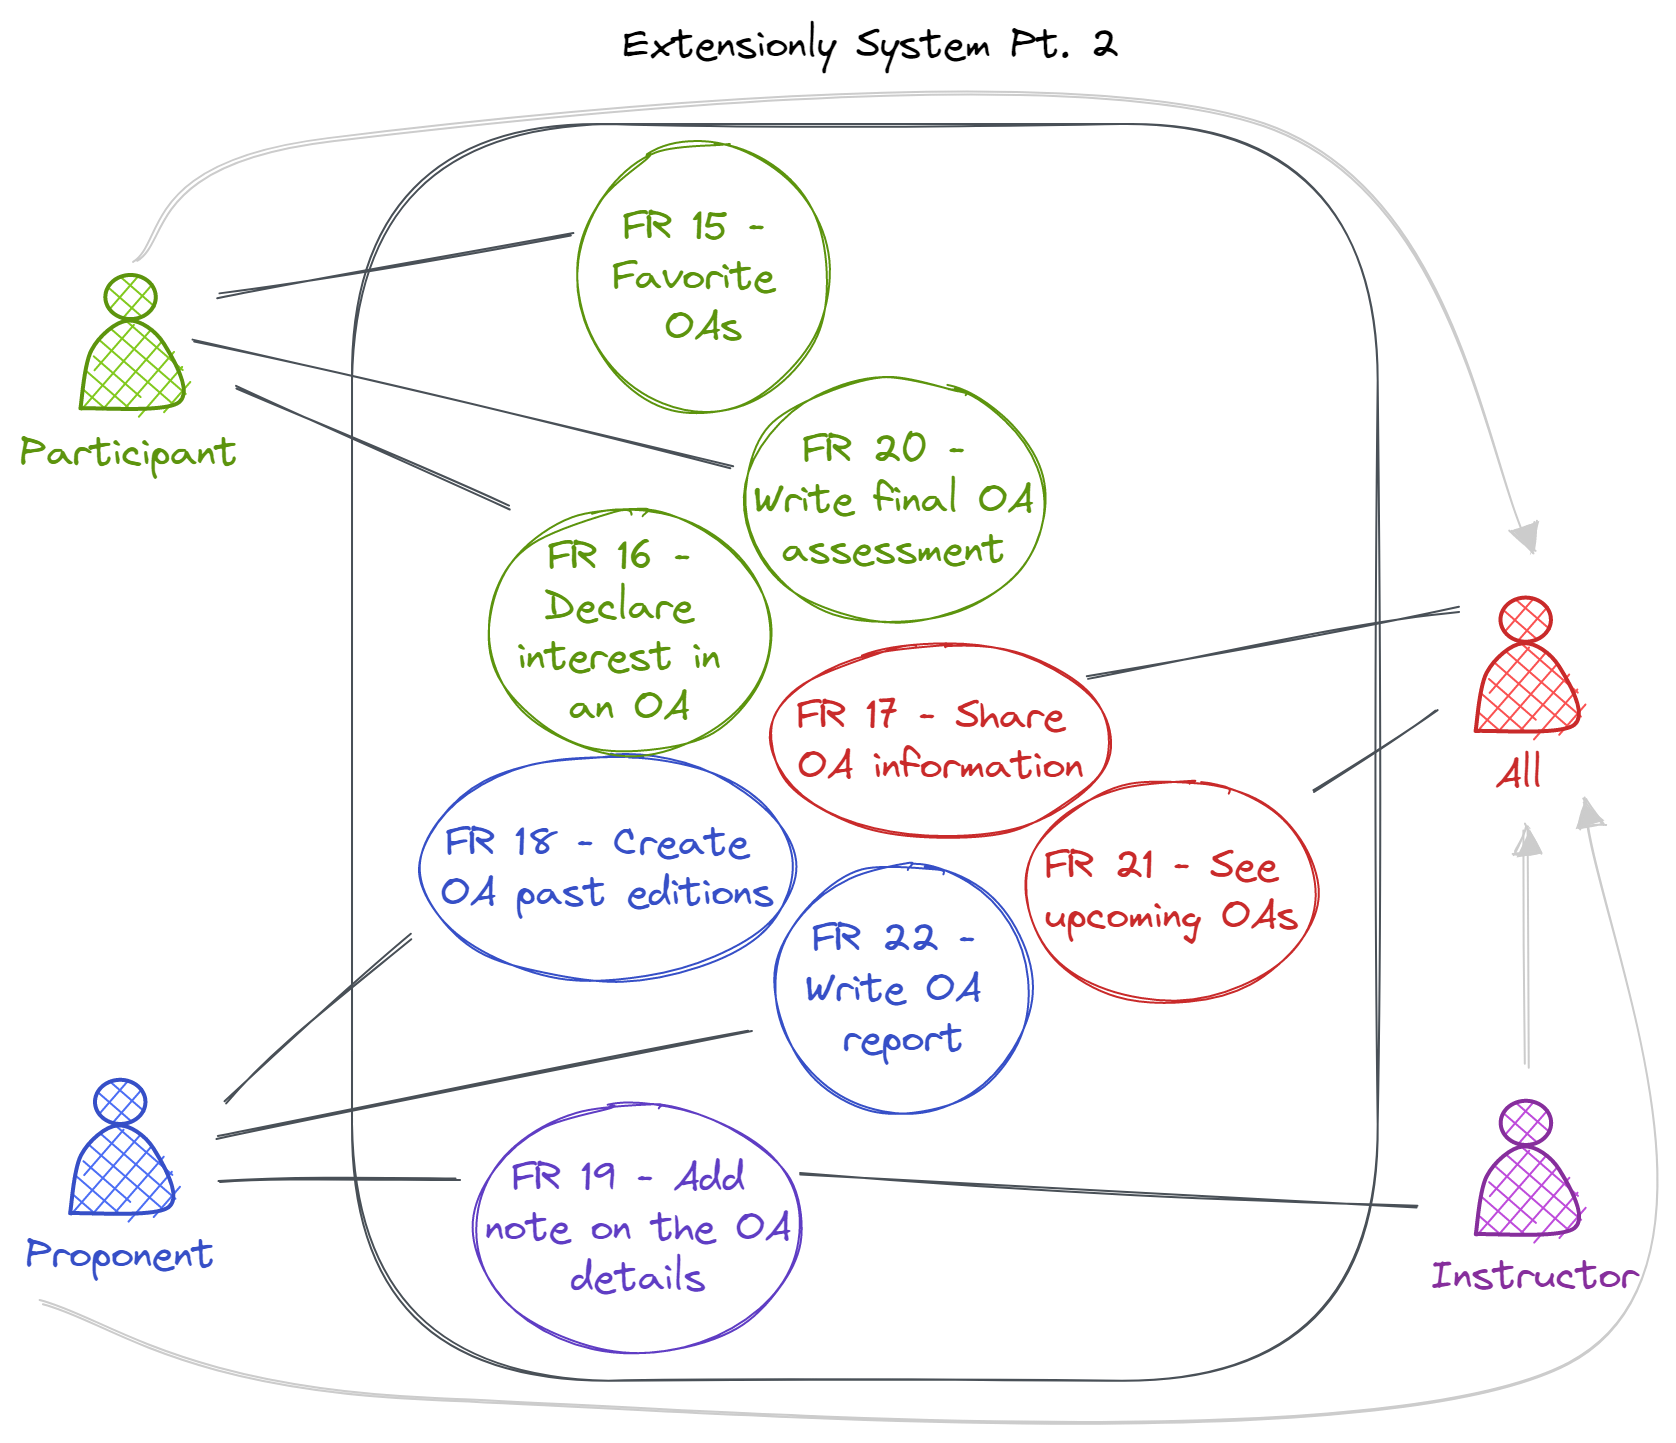
\includegraphics[width=12cm]{img/6-use-case-2.png}
  \end{center}
  \fonte{Author.}
\end{figure}

\subsection{User Stories Derived from the Requirements}
% ===================================
% Para o survey ser aplicado, um modelo de pergunta deveria ser montado com que a maioria dos respondentes compreendessem a mensagem a ser passada. 
% Para isso utilizando o modelo de historias de usuario que busca apresentar o papel do usuario, que vai desempenhar aquele determinado requisito, o objetivo da historia e o motivo por traz. 

For the survey to be applied, a question template should be set up so that most respondents understand the message to be conveyed. The user stories were derived from the \aclp{FR} presented by \Cref{tab:initial-requirements} and were divided between the roles of the system users. \Cref{tab:proponent-user-stories} shows user stories related to the proposer, then \cref{tab:instructor-user-stories} shows those related to the instructor, \Cref{tab:participant-user-stories} lists those related to the participant, and finally the \Cref{tab:coordinator-user-stories} contains the coordinator's user stories.

\begin{table}[!htb]
  \centering
  \setlength{\aboverulesep}{0pt}
  \setlength{\belowrulesep}{0pt}
  \caption{Proponent User Stories}
  \label{tab:proponent-user-stories}
  \footnotesize
  \begin{tabularx}{\textwidth}{c|X}
    \toprule
    \rowcolor[rgb]{0.753,0.753,0.753} \textbf{ID} & \textbf{User Story}                    \\
    \hline
    \rowcolor[rgb]{0.898,0.898,0.898} P1          & As a Proponent, I would like to propose an outreach activity, creating knowledge opportunities for other people.                                           \\
    P2                                            & As a Proponent, I would like to define desired prerequisites for enrollment in my outreach activity proposal, so that my applicants do not come unprepared.                                      \\
    \rowcolor[rgb]{0.898,0.898,0.898} P3          & As a Proponent, I would like my data to be shown along the details page of my outreach activity, so that participants have more details of who I am.                                \\
    P4                                            & As a Proponent, I would like to leave comments on the outreach activity page, to request some special material for carrying out the activity or just leave a note of mine for the participants.                              \\
    \rowcolor[rgb]{0.898,0.898,0.898} P5          & As a Proponent, I would like to fill in a general report on the progress of the outreach activity carried out, for archiving purposes.                                \\
    P6                                            & As a Proponent, I would like to register multiple editions of the same outreach activity, so that new participants can check past editions.                              \\
    \rowcolor[rgb]{0.898,0.898,0.898} P7          & As a Proponent or Instructor, I would like to get in touch with the participants of the outreach activity, so that it is easy to pass on information relevant to the activity.                                \\
    P8                                            & As a Proponent, I would like to receive the evaluation of the participants of my outreach activity in a detailed report/form format, so that I am aware of what I should improve for the next edition.                              \\
    \bottomrule
  \end{tabularx}
\end{table}
\begin{table}[!htb]
  \centering
  \setlength{\aboverulesep}{0pt}
  \setlength{\belowrulesep}{0pt}
  \caption{Instructor User Stories}
  \label{tab:instructor-user-stories}
  \footnotesize
  \begin{tabularx}{\textwidth}{c|X}
    \toprule
    \rowcolor[rgb]{0.753,0.753,0.753} \textbf{ID} & \textbf{User Story}         \\
    \hline
    \rowcolor[rgb]{0.898,0.898,0.898} I1          & As an Instructor, I would like to manage the attendance of registered participants so that certificates can be issued for those present.                                           \\
    \bottomrule
  \end{tabularx}
\end{table}
\begin{table}[!htb]
  \centering
  \setlength{\aboverulesep}{0pt}
  \setlength{\belowrulesep}{0pt}
  \caption{Participant User Stories}
  \label{tab:participant-user-stories}
  \footnotesize
  \begin{tabularx}{\textwidth}{c|X}
    \toprule
    \rowcolor[rgb]{0.753,0.753,0.753} \textbf{ID} & \textbf{User Story}                   \\
    \hline
    \rowcolor[rgb]{0.898,0.898,0.898} A1          & As a Participant, I would like to apply for outreach activities such as events, courses and lectures, to enter the waiting list and be accepted in the activity.                                          \\
    A2                                            & As a Participant, I would like to be able to search for outreach activities, so that I can find what I am looking for more easily.                                     \\
    \rowcolor[rgb]{0.898,0.898,0.898} A3          & As a Participant, I would like to cancel or edit the information of an outreach activity enrollment made by me, to have more freedom in case I change my mind.                                \\
    A4                                            & As a Participant, I would like to see previous editions of outreach activities, so that I can read past proposals.                              \\
    \rowcolor[rgb]{0.898,0.898,0.898} A5          & As a Participant, I would like to view the history of all the outreach activities I have participated in, so that I don't have to keep the record outside of the tool.                                \\
    A6                                            & As a Participant, I would like to have a help area within the system, to guide me with any questions or problems that I may face with the activity I signed up for.                              \\
    \rowcolor[rgb]{0.898,0.898,0.898} A7          & As a Participant without college enrollment, I would like to register in the system to participate in outreach activities that interest me.                                \\
    A8                                            & As a Participant, I would like to inform my interest in areas of knowledge, so that I can see outreach activities related to them.                              \\
    \rowcolor[rgb]{0.898,0.898,0.898} A9          & As a Participant, I would like to favor outreach activities that I deem interesting, so that I have easy access to them when I need them.                                \\
    A10                                           & As a Participant, I would like to show my interest in unavailable outreach activities, so that I will be notified when a new issue opens.                              \\
    \rowcolor[rgb]{0.898,0.898,0.898} A11         & As a Participant, I would like to register for outreach activities without registering in the system, so that my information is not saved.                                \\
    A12                                           & As a Participant, I would like to share information about the outreach activity, so that I can share it more easily with my friends.                              \\
    \rowcolor[rgb]{0.898,0.898,0.898} A13         & As a Participant, I would like to evaluate the outreach activity in which I participated, so that other participants can see the grade I assigned.                                \\
    A14                                           & As a Participant, I would like to see the outreach activities in which I am enrolled in the form of a calendar, so that I can organize myself better.                              \\
    \bottomrule
  \end{tabularx}
\end{table}
\begin{table}[!htb]
  \centering
  \setlength{\aboverulesep}{0pt}
  \setlength{\belowrulesep}{0pt}
  \caption{Coordinator User Stories}
  \label{tab:coordinator-user-stories}
  \footnotesize
  \begin{tabularx}{\textwidth}{c|X}
    \toprule
    \rowcolor[rgb]{0.753,0.753,0.753} \textbf{ID} & \textbf{User Story}         \\
    \hline
    \rowcolor[rgb]{0.898,0.898,0.898} C1          & As Coordinator, I would like to manage the submissions of new outreach activities carried out, so that each proposal goes through a review process before being accepted.                                           \\
    C2                                            & As Coordinator, I would like to issue certificates of participation with a certain number of hours for all involved, participants, instructors and coordinator, so that the individual's involvement in the outreach activity is proven.                                     \\
    \bottomrule
  \end{tabularx}
\end{table}
% ===================================

% ===================================
They were applyed directly, with no other refinements, in the final survey and can be seen in \Cref{appendix:questionnaire}.
However, in order to relate \acp{FR} with the questions and also update their ranking based on the survey results, \Cref{tab:stories-requirements-relation} was created.
% ===================================

\begin{table}[!htb]
  \centering
  \setlength{\aboverulesep}{0pt}
  \setlength{\belowrulesep}{0pt}
  \caption{Requirements vs User Stories Priorities}
  \label{tab:stories-requirements-relation}
  \footnotesize
  \begin{tabular}{c|c|c}
    \toprule
    \rowcolor[rgb]{0.753,0.753,0.753} \textbf{Requirement ID} & \textbf{Question/Story ID} & \textbf{Priority} \\
    \hline
    \rowcolor[rgb]{0.898,0.898,0.898} FR. 01                  & P1                         & Must have         \\
    FR. 02                                                    & A1                         & Must have         \\
    \rowcolor[rgb]{0.898,0.898,0.898} FR. 03                  & I1                         & Must have         \\
    FR. 04                                                    & C1                         & Must have         \\
    \rowcolor[rgb]{0.898,0.898,0.898} FR. 05                  & A2                         & Must have         \\
    FR. 06                                                    & P2                         & Should have       \\
    \rowcolor[rgb]{0.898,0.898,0.898} FR. 07                  & A3                         & Must have         \\
    FR. 08                                                    & A5                         & Must have         \\
    \rowcolor[rgb]{0.898,0.898,0.898} FR. 09                  & A5                         & Must have         \\
    FR. 10                                                    & A6                         & Must have         \\
    \rowcolor[rgb]{0.898,0.898,0.898} FR. 11                  & A2                         & Must have         \\
    FR. 12                                                    & A11                        & Will not have     \\
    \rowcolor[rgb]{0.898,0.898,0.898} FR. 13                  & A8                         & Must have         \\
    FR. 14                                                    & P3                         & Should have       \\
    \rowcolor[rgb]{0.898,0.898,0.898} FR. 15                  & A9                         & Must have         \\
    FR. 16                                                    & A10                        & Must have         \\
    \rowcolor[rgb]{0.898,0.898,0.898} FR. 17                  & A12                        & Should have       \\
    FR. 18                                                    & P6                         & Must have         \\
    \rowcolor[rgb]{0.898,0.898,0.898} FR. 19                  & P4                         & Should have       \\
    FR. 20                                                    & A13                        & Should have       \\
    \rowcolor[rgb]{0.898,0.898,0.898} FR. 21                  & A14                        & Must have         \\
    FR. 22                                                    & P5                         & Should have       \\
    \bottomrule
  \end{tabular}
\end{table}

\subsection{Roles}\label{ext:roles}
% ===================================
% Para o servico funcionar corretamente e de uma maneira organizada foram criados papeis de usuarios, controlando o que cada um pode ou não desempenhar dentro da ferramenta. 
% Estes papeis foram pensados tomando em conta os atuais papeis que existem relacionados a \acp{OA} dentro de uma \acp{HEI}, os papeissão os seguintes: 
% \begin{inparaenum}[(1)]
%   \item Participant - a listener, someone who enrolls to passively participate in the activity;
%   \item Instructor - a speaker, someone who presents or teaches something to participants;
%   \item Proponent - the one who proposes the \ac{OA}, usually a professor;
%   \item Coordinator - a role that can review and approve proposed activities for one campus;
%   \item Supervisor - usually does not interact with the process, but can monitor the system as a whole, having access to \ac{OA} in multiple campuses.
% \end{inparaenum}

For the service to work correctly and in an organized way, user roles were created, controlling what each one can or cannot perform within the tool.
These roles were designed taking into account the current roles that exist related to \acp{OA} within an \acp{HEI}, the roles are the following:
\begin{inparaenum}[(1)]
  \item Participant - a listener, someone who enrolls to passively participate in the activity;
  \item Instructor - a speaker, someone who presents or teaches something to participants;
  \item Proponent - the one who proposes the \ac{OA}, usually a professor;
  \item Coordinator - a role that can review and approve proposed activities for one campus;
  \item Supervisor - usually does not interact with the process, but can monitor the system as a whole, having access to \ac{OA} in multiple campuses.
\end{inparaenum}
% ===================================

% ===================================
% Além dos papeis citados acima, outro que não esta dentro do escopo do \ac{MVP} foi pensado, este é o ``External Participant'', que tem permissões semelhantes ao Participant, mas é uma pessoa que não tem relação direta com a universidade, mas que consegue se inscrever em atividades de extensão da mesma maneira.

In addition to the roles mentioned above, another that is not within the scope of \ac{MVP} was thought, this is the ``External Participant'', which has similar permissions to the Participant, but is a person who has no direct relationship with the university, but who manages to enroll in \aclp{OA} in the same way.
% ===================================
% Participant
% Instructor
% Proponent
% Coordinator
% Supervisor
% External

\section{Design Decisions}\label{sec:ext-design}
% ===================================
This section describes the design decisions taken to carry out this study and the development of this tool:
\begin{description}
    % \item[\textbf{Programming Language:}] \ac{TS} foi escolhido porque ela fornece diversas soluções e frameworks disponiveis para uso, que simplificam o desenvolvimento. Um ponto positivo e que se destaca da linguagem base \ac{JS}, é que esta linguagem adiciona tipagem estática ao código, reduzindo muito as chances de erro por sintaxe e agilizando o desenvolvimento. Outro fator de escolha se da pela experiencia dos desenvolvedores, que ja estão familiarizados com esta linguagem e seus frameworks, a mesma linguagem foi escolhida no frontend, facilitando o entendimento entre os códigos fonte.  
    
    \item[\textbf{Programming Language:}] \ac{TS} was chosen because it enriches \ac{JS} with a module system, classes, interfaces, and a static type system, as said by \textcite{Bierman_2014}.
    The authors also comments that a typed language helps a lot in development, finding and preventing bugs, providing auto-completion, hover tips, navigation through the code, and also helps in code refactoring.
    % A positive point that stands out from the base language \ac{JS} is that this language adds static typing to the code, greatly reducing the chances of syntax errors and speeding up development. 
    Another choice factor is given by the experience of the developers, who are already familiar with this language and its frameworks, the same language was chosen in the frontend, facilitating the understanding between the source codes;
    % ===================================
    
    % ===================================
    % \item[\textbf{Framework:}] NestJS desenvolvido por \cite{nestDocs}, foi o framework escolhido devido o seu potencial e facilidade em escalabilidade de aplicações. Ele possui uma organizaçao de arquivos muito simples, chamada de model-service-controller, onde a camada model é responsavel pelo gerenciamento de dados, controller é responsável pelo gerenciamento de entradas e saidas de requisiçoes na nossa aplicaçao e a camada service contém toda a lógicade implementação, parte dessa organizaçao pode ser vista na \Cref{fig:architecture}.
    
    \item[\textbf{Framework:}] NestJS developed by \textcite{nestDocs}, was the chosen framework due to its potential and ease of application scalability. The author also mention that it has a very simple file organization, called model-service-controller, where the model layer is responsible for managing data, controller is responsible for managing input and output requests in our application and the service layer contains all the logic of implementation, part of this organization can be seen in \Cref{fig:architecture};
    % ===================================
    
    % ===================================
    % Outro ponto muito forte do NestJS é o seu suporte a modularização, em que mesmo que o código seja escrito de uma maneira monolítica, as controllers e servicos estarão separadas por responsabilidades, facilitando uma possivel futura transição entre arquiteturas. Combinado a modularizaçao, este framework fornece um poderoso sistema de injeção de dependencias permitindo que códigos sejam reutilizados entre módulos de maneira muito simples, basta injeta-lo no modulo destino.
    
    Another very strong point of NestJS is its support for modularization, as demonstrated by \textcite{nestDocs},  in which even if the code is written in a monolithic way, the controllers and services will be separated by responsibilities, facilitating a possible future transition between architectures. Combined with modularization, this framework provides a powerful dependency injection system allowing code to be reused between modules in a very simple way, just inject it into the target module;
    % ===================================
    
    % ===================================
    % Em relaçao a persistencia de dados, o NestJS permite a utilização de \acp{ORM}, que facilitam esta interaçao com os bancos de dados, ficando ele responsavel por todas as complicaçoes envolvidas neste processo, mais sobre o assunto sera explicado no \Cref{data-persistance}.
    
    Regarding data persistence, Nest allows the use of \acp{ORM}, which are, as \textcite{Wiphusitphunpol_2017} said, a tool for mapping database query results to strongly typed or weakly typed objects in object-oriented programming languages, increasing the speed of development and maintainability. More on the subject will be explained in \Cref{data-persistence};
    % ===================================
    
    % ===================================
    % \item[\textbf{Architecture:}] A arquitetura escolhida para o desenvolvimento da Extensionly foi server-client model que de acordo com \textcite{puliafito_riccobene_scarpa}, é uma arquitetura que dispõe servicos ou servidores duplicados para uma rede de clientes que os utilizam. 
    
    \item[\textbf{Architecture:}] The architecture chosen for the development of Extensionly was the server-client model which, according to \textcite{puliafito_riccobene_scarpa}, is an architecture that has duplicated services or servers for a network of clients that use them.
    % ===================================
    
    % ===================================
    % Na \Cref{fig:architecture} está representado a arquitetura pensada para este \ac{MVP}, ainda há possibilidades de melhoria como por exemplo, adicionar um Load Balancer entre as chamadas do cliente para o servidor, sendo responsável por duplicar as instâncias existentes do servidor caso haja um pico de acessos na aplicação. Outra melhoria está na adição de cache nas chamadas para o banco de dados, que serve para acessar mais rapidamente dados que estão sendo requisitados com frequencia.
    
    The architecture designed for this \ac{MVP} is represented in \Cref{fig:architecture}, there are still possibilities for improvement, such as adding a server load balancer between client calls to the server, being responsible for spreading out the transmission of information flow and data operations, as well as lowering the risk of information loss and computing time, as \textcite{Chen_2015} described.
    Another improvement is the addition of caching in calls to the database, which serves to more quickly access data that is being requested frequentl.
    % ===================================
    
    \begin{figure}[htb]
      \caption{Backend Achitecture}\label{fig:architecture}
      \begin{center}
        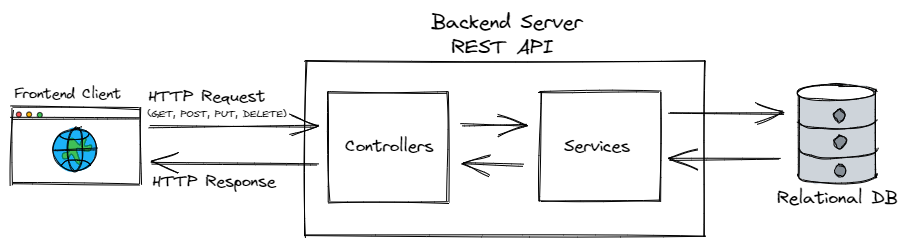
\includegraphics[width=15cm]{img/6-architecture.png}
      \end{center}
      \fonte{Author.}
    \end{figure}
    
    % ===================================
    % O servidor backend utiliza a arquitetura API Rest, onde \ac{API}, de acordo com \textcite{restApi}, utiliza de requisições \ac{HTTP} como: 
    % \begin{inparaenum}[(1)]
    %   \item GET;
    %   \item POST;
    %   \item PUT;
    %   \item DELETE, 
    % \end{inparaenum} para realizar a manipulaçao de dados do sistema. Em seguida, o autor define \ac{REST} como restrições utilizadas para que as requisições \ac{HTTP} atendam as diretrizes definidas na arquitetura, dentre elas estão:
    % \begin{inparaenum}[(1)]
    %   \item Utilizar arquitetura cliente-servidor;
    %   \item Não possuir estado, requisiçoes sendo independentes;
    %   \item Possuir cache;
    %   \item Possuir uma nterface uniforme.
    % \end{inparaenum}
    
    The backend server uses the REST API architecture, where \ac{API}, according to \textcite{restApi}, uses \ac{HTTP} requests such as:
    \begin{inparaenum}[(1)]
      \item GET;
      \item POST;
      \item PUT;
      \item DELETE, 
    \end{inparaenum} to perform system data manipulation. Then, \textcite{restApi} defines \ac{REST} as restrictions used so that \ac{HTTP} requests meet the guidelines defined in the architecture, among them are:
    \begin{inparaenum}[(1)]
      \item Use server-client architecture;
      \item Not having state, requests being independent;
      \item Have cache;
      \item Have a uniform interface;
    \end{inparaenum}
    % ===================================
    
    % Client Server
    % API
    % Diretrizes REST
    % ===================================
    % \item[\textbf{License:}] A ferramenta Extensionly sera em um primeiro momento uma soluçao Open Source, ja que desta maneira outras pessoas poderão contribuir com a aplicação. Entretanto existe a possíbilidade de que a aplicaçao seja fornecida em modelo de serviço no futuro, logo funcionalidades pagas podem ser adicionadas.
    
    \item[\textbf{License:}] The Extensionly backend is licensed under the GNU General Public License v3.0, which is an open source license and is very permissive, allowing even for commercial use. However, it is very important to keep in mind that all works and modifications must be released under the same license, with the source code made available, and that the distribution of closed source versions is not permitted. Additionally, it does not provide the software with any guarantees or liabilities \cite{gnugpl3}.
    
    % ===================================
    % Open-source
    % Futuramente Pago algumas funcionalidades
    % ===================================
    % \item[\textbf{Data Persistence:}]\label{data-persistance}
    % Para realizar a persistencia dos dados, será utilizado banco de dados relacional, que é o mais adequado ao carater do problema por ter muitas relaçoes entre os objetos presentes no sistema, para isso será utilizado o \ac{DBMS} \ac{MySQL}.
    \item[\textbf{Data Persistence:}]\label{data-persistence} To perform the data persistence, a relational database will be used, which is the most suitable for this problem because it has many relationships between the objects present in the system, for which \ac{DBMS} \ac{MySQL} will be used.
    % ===================================
    
    % ===================================
    % Também sera utilizado o Prisma como o \ac{ORM} da ferramenta, que de acordo com \textcite{prisma}, is an \ac{ORM} that helps app developers build faster and make fewer errors, disponibilizando um schema do banco de dados que allows developers to define their application models in an intuitive data modeling language, reducing boilerplate so developers can focus on the important parts of the app.
    
    Prisma will also be used as the \ac{ORM} of the tool, which according to \textcite{prisma}, is an \ac{ORM} that helps app developers build faster and make fewer errors, providing a database schema which allows developers to define their application models in an intuitive data modeling language, reducing boilerplate so developers can focus on the important parts of the app;
    % ===================================
    % Banco relacional
    % MySQL
    % Prisma
    % ===================================
    % \item[\textbf{DevOps:}] Para que a aplicação seja automatica quando se trata de build, testes e deploy, serão utilizadas algumas soluçoes de DevOps, comecando com as pipelines do GitHub Actions, que são muito simples para o entendimento e ja estão alocadas junto com o repositório\footnote{Extensionly Backend code is available at \url{https://github.com/IgorDalepiane/extensionly-backend-service}} do backend. 
    % Com as pipelines é possível bloquear um \ac{PR} até que o código para ser adicionado esteja de acordo com as diretrizes definidas, realizar o deploy quando determinadas açoes acontecem, testar codigo automaticamente, tudo isso melhora o controle e organizaçao do código, será utilizado como base o tutorial\footnote{CICD Tutorial is available at \url{https://github.com/IgorDalepiane/CICD-Tutorial/wiki}} feito pelo autor.
    
    
\end{description}

\section{\ac{DevOps}}\label{sec:dev-ops}

\textcite{perera2017improve} describes \ac{DevOps} as a set of techniques that allows developers and operators to interact and work together to provide software and services quickly, consistently, and of higher quality. The solution chosen was the GitHub Actions, which are very simple to understand and already are allocated along with the backend repository.

% ========================================================
% Integrado a prática de DevOps o autor \textcite{Shahin_2017} explica três diferentes termos muito importantes para o entendimento do funcionamento desta prática, a estrutura da pipeline e do funcionamento na prática destes termos esta representada na \Cref{fig:relationship-ci-cde-cd}, os termos são os que seguem:

Integrated into the \ac{DevOps} practice, the author \textcite{Shahin_2017} explains three different terms that are very important to understand how this practice works, the structure of the pipeline and how these terms work in practice is represented in \Cref{fig:relationship-ci-cde-cd}, the terms are as follows:
% ========================================================

\begin{description}
    % ========================================================
    % \item[\textbf{\ac{CI}}] A definiçao do termo diz a respeito de times de desenvolvimento mergearem trabalho de desenvolvimento com mais frequencia, aumentando a qualidade do produto, o desempenho do time e reduzindo prazos de entrega, incluindo passos de build e testes automatizados.
    
    \item[\textbf{\ac{CI}}] The definition of the term is about development teams merging development work more frequently, increasing product quality, team performance and reducing delivery times, including steps of build and automated tests.
    
    % ========================================================
    % \item[\textbf{\ac{CDE}}] Este termo representa o processo que garante que a aplicação vai sempre estar em um estado pronto para ser enviada para produçao, passando em pipelines com testes automatizados e checagens de qualidade. Esta prática reduz o esforço necessário e riscos envolvidos na hora de enviar um software para produçao.
    
    \item[\textbf{\ac{CDE}}] This term represents the process that guarantees that the application will always be in a state ready to be sent to production, passing through pipelines with automated tests and quality checks. This practice reduces the effort required and risks involved when sending software to production.
    % ========================================================
    % \item[\textbf{\ac{CD}}] Este termo pode ser muito semelhante ao anterior, pois busca fazer as mesmas coisas mas de uma maneira mais automatica, enquanto o item anterior necessita da ação humana para aprovar um deploy para produçao, este termo utiliza de pipelines que enviam diretamente qualquer mudança de código mergeada, para o ambiente real de produção.
    
    \item[\textbf{\ac{CD}}] This term can be very similar to the previous one, as it seeks to do the same things but in a more automatic way, while the previous item needs human action to approve a deploy for production, this term uses pipelines that send any merged code changes directly to the real production environment.
    % ========================================================
\end{description} 

\begin{figure}[htb]
  \caption{The relationship between continuous integration, delivery and deployment}\label{fig:relationship-ci-cde-cd}
  \begin{center}
    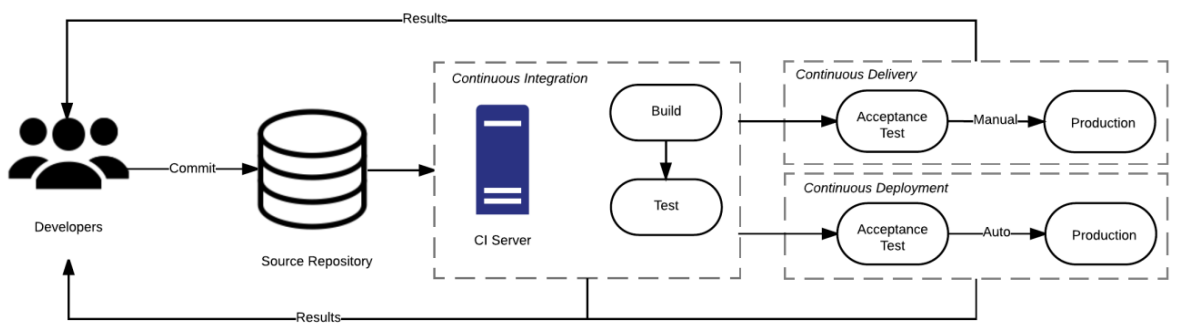
\includegraphics[width=15cm]{img/6-ci-cde-structure.png}
  \end{center}
  \fonte{\cite{Shahin_2017}.}
\end{figure}
% ========================================================
% Os termos que serão implementados no backend da ferramenta Extensionly serão o \ac{CI} e o \ac{CDE}, pois assim é possivel ter mais controle no versionamento da solução, e sempre mantendo ela testada e pronta para ser enviada para produçao.

The terms that will be implemented in the backend of the Extensionly tool will be \ac{CI} and \ac{CDE}, because this way it is possible to have more control in the versioning of the solution, and always keeping it tested and ready to be sent to production.
% ========================================================
% Para que a aplicaçao de DevOps funcione corretamente uma boa configuraçao de repositório, projetos, deploys e pipelines deve ser executada, para isso sera utilizado o tutorial\footnote{CICD Tutorial is available at \url{https://github.com/IgorDalepiane/CICD-Tutorial/wiki}} desenvolvido pelo autor deste \ac{TP}.

For the \ac{DevOps} application to work correctly, a good configuration of repository, projects, deploys and pipelines must be performed, for this will be used the tutorial\footnote{CICD Tutorial is available at \url{https://github.com/IgorDalepiane /CICD-Tutorial/wiki}} developed by the author of this \ac{TP}.
% ========================================================

% With pipelines it is possible to block a \ac{PR} until the code to be added complies with the defined guidelines, perform the deployment when certain actions happen, test code automatically, all this improves the control and organization of the code, it will be used as a basis the tutorial\footnote{CICD Tutorial is available at \url{https://github.com/IgorDalepiane/CICD-Tutorial/wiki}} made by the author.
% ===================================
% ===================================
% Para a realizaçao do deploy, será utilizado o Hiroku, que é uma solução gratis e muito eficaz, sendo o suficiente para o proposito deste \ac{MVP}.

For the deployment, Heroku will be used, which according to \textcite{heroku} is a cloud platform that lets developers build, deliver, monitor and scale apps. Heroku's \ac{PaaS} service will be used, which according to \textcite{Zvarevashe2014TheAO}, is a service that allows the contractor to publish their applications in the cloud without having to install any software on their local machine, it also already solves configurations related to infrastructure and machine configurations, allowing the developer to focus only on the development of the tool.
% ===================================
% Pipelines, testes, build
% Deploy, Netlify, Vercel ou Hiroku

\section{Chapter Summary}
% ===================================
% Este capitulo discorreu sobre decisões relacionadas a produção da ferramenta Extensionly, primeiro sendo explicado alguns pontos de atenção na \Cref{sec:ext-considerations}, logo na \Cref{sec:ext-req}, foram apresentados os requisitos finais levantados pela literatura cinza e as estorias de usuario com as suas pontuaçoes recebidas pela execução do survey. Por fim, \Cref{sec:ext-design} reporta as decisoes de design para a execução do projeto, como tecnologias e arquitetura utilizada.

This chapter discussed decisions related to the production of the Extensionly tool, first explaining some points of attention in \Cref{sec:ext-considerations}, then in \Cref{sec:ext-req}, the final requirements raised by grey literature review and user stories with their scores received for carrying out the survey, are shown. \Cref{sec:ext-design} reports the design decisions for the execution of the project, such as technologies and architecture used. Finally, in \Cref{sec:dev-ops}, some terms related to \ac{DevOps} were discussed, along with the choices that will be used in the tool development processes.

% ===================================


% \section{Requirement Engineering}
% \subsection{Requirements Elicitation, Modeling and Analysis}
% \subsection{User Stories}

% \section{Features}
% \begin{landscape}
\begin{figure}[!htb]
\caption{Taxonomy of performance testing tools represented by feature model.}
\label{fig:featuremodel}
\begin{adjustbox}{max width=1.5\textwidth}
%% https://tex.stackexchange.com/questions/335708/feature-diagram-in-latex
    \begin{forest}  
    disjunction tree,
    disjuncts from'=1,
    concrete from'=1,
    concrete colour=blue!55!cyan!40,
    abstract colour=blue!85!cyan!15,
    draw colour=darkgray,
    [Performance Testing Process
        [Profiles/Roles, mandatory, l=25mm
            [Performance Engineer, l=20mm
                [Architect, l=20mm]
                [Tester, l=20mm]
                [Analyst, l=20mm]
            ]
        ]
        [Methods, mandatory, l=25mm
            [Scripting, l=20mm]
            [CR, l=20mm]
            [MBT, l=20mm]
        ]
        [Artifacts, mandatory, l=25mm
            [Test Plan, optional, l=20mm]
            [Model, optional, l=20mm]
            [Script, l=20mm]
            [Workload, l=20mm]
            [Scenario, l=20mm]
            [Test Report, l=20mm]
        ]
        [Approaches, mandatory, l=25mm,
            [Load, l=20mm]
            [Stress, l=20mm]
            [Endurance, l=20mm]
            [Spike, l=20mm]
        ]
        [Stages, mandatory, l=71mm
            [Pre-Test, mandatory, l=20mm
                [Planning, optional, l=20mm]
                [Scripting, l=20mm]
                [Design, l=20mm]
                [Configuration, l=20mm]
            ]
            [Test, mandatory, l=20mm
                [Execution, l=20mm]
                [Monitoring, l=20mm]
            ]
            [Post-Test, mandatory, l=20mm
                [Analysis, optional, l=20mm]
                [Reporting, l=20mm]
            ]
        ]
    ]
    \end{forest}
    \end{adjustbox}
    \centering
    \fonte{Author.}
    \end{figure}
\end{landscape}
% \subsection{Roles}

% \section{Development}
% \subsection{Technology Stack}
% \subsection{Programming Paradigm}
% \subsection{Design Patterns}

% \section{Software Architecture}
% \subsection{DevOps}
% \subsection{Pipeline}

% \section{Testing}

% \section{Software Artifacts}
% \subsection{Domain Model}
% \subsection{Component Diagram}
% \subsection{Database Schema}
  % 03/08
%==============================================================================
\chapter{PRELIMINARY CONCLUSIONS}\label{conclusions}
%==============================================================================
% 1-Recapitular o tema do trabalho, aspectos da justificativa, motivos de escolha do tema, contribuições do trabalho
% 1-Metodologia do trabalho
% Esse trabalho pretendeu entender [apresente o tema] para [justificativa do trabalho], a partir de [metodologia utilizada].
%==============================================================================
% O presente trabalho buscou se aprofundar em processos de gerenciamento de atividades de extensão, para construir uma ferramenta que de suporte nos processos burocraticos envolvidos, facilite a comunicação com a comunidade externa, e aumente a divulgação e integração dos alunos com as atividades. Para isso utilizou-se de duas metodologias, uma revisão na literatura cinza para encontrar soluções similares ja existentes elicitando as suas funcionalidades principais, e um survey com os possíveis usuários finais da ferramenta, em busca de ordenar os requisitos baseado em sua importância, também adiquirindo mais sugestões relacionadas ao assunto.

The present work sought to delve into processes of management of \aclp{OA}, to build a tool that supports the bureaucratic processes involved, facilitates communication with the external community, and increases the dissemination and integration of students with the activities. 
For this, two methodologies were used, a review in the grey literature to find similar solutions that already exist, eliciting their main functionalities, and a survey with the possible end users of the tool, in search of ordering the requirements based on their importance, also acquiring more suggestions related to the subject.
%==============================================================================

%==============================================================================
% 2-Objetivos do TCC, atingiu os objetivos? explicar a opinião
% Para se atingir uma compreensão do [objetivo geral], definiu-se três objetivos específicos. O primeiro [objetivo específico]. Verificou-se que [resultado]. Depois, [objetivo específico 2]. A análise permitiu concluir que [resultado].
%==============================================================================
%==============================================================================
% 3 - apresentar resultados obtidos(sem dados), não pode aparecer nenhuma informação NOVA, 
% 3 - Avanços em relação aos objetivos definidos
%==============================================================================
% Para ser possivel atingir o objetivo geral do trabalho, que é Develop the backend of the tool to support the management of outreach programs and projects of \ac{UNIPAMPA}, foram definidos cinco objetivos especificos. 
% O primeiro objetivo era de realizar a revisão na literatura cinza em busca de funcionalidades em ferramentas similares, com os resultados obtidos pode-se verificar que este foi atingido, pois foi possível levantar diversas ferramentas e no final sair com uma lista de tamanho significante juntamente com suas funcionalidades e detalhes especificos, contribuindo muito no planejamento.  
% O segundo objetivo esta relacionado com a elaboração de um survey para compreender as opiniões dos possíveis usuários finais, este objetivo foi atingido com sucesso pois foi possivel analisar as dores e preocupações dos usuários, sendo possível com os resultados, extrair várias melhorias e funcionalidades para a ferramenta proposta.

In order to achieve the general objective of the work, which is develop the backend of the tool to support the management of outreach programs and projects of \ac{UNIPAMPA}, five specific objectives were defined.
The first objective was to carry out a review in the grey literature in search of features in similar tools, with the results obtained it can be seen that this was achieved, as it was possible to raise several tools and in the end to come out with a list of significant size together with its functionalities and specific details, contributing a lot in planning.
The second objective is related to the elaboration of a survey to understand the opinions of the possible end users, this objective was successfully achieved because it was possible to analyze the pains and concerns of the users, being possible with the results, to extract several improvements and functionalities for the proposed tool.

%==============================================================================
% A construção de um roadmap e tasks concretas para o desenvolvimento, define o terceiro objetivo especifico, este foi atingido de modo parcial pois a transformação de \ac{FR} para tarefas de desenvolvimento apenas ocorrerá no desenvolvimento da segunda parte deste trabalho, durante o \ac{TP} II. 
% O quarto objetivo diz sobre o estudo, analise e escolha de uma stack de desenvolvimento para o backend da ferramenta proposta, incluindo linguagem de programação, arquiteturas e frameworks, este objetivo foi atingido com sucesso, as escolhas feitas podem ser vistas na \Cref{extensionly}. 
% Como quinto e ultimo objetivo especifico está no próprio desenvolvimento de um \ac{MVP} do backend da ferramenta, este objetivo ainda não foi atingido, pois está planejado que o desenvolvimento venha a acontecer ainda.

The construction of a roadmap and concrete tasks for the development, defines the third specific objective, this was partially achieved because the transformation from \ac{FR} to development tasks will only occur in the development of the second part of this work, during the \ac{TP} II.
The fourth objective says about the study, analysis and choice of a development stack for the backend of the proposed tool, including programming language, architectures and frameworks, this objective was successfully achieved, the choices made can be seen in \Cref{extensionly}.
As the fifth and last specific objective is the development of an \ac{MVP} for the tool's backend, this objective has not yet been achieved, as it is planned that the development will happen yet.
%==============================================================================
% 4 - Verificar a hipotese, confirmou ou refutou? explicar
% Com isso, a hipótese do trabalho de que [hipótese] se [ confirmou ou se refutou], por [motivos].
%==============================================================================
% Com os objetivos e resultados analisados, a hipotese deste trabalho de que ``With a tool to support the management of outreach programs and projects, it’s possible to have a reduction on the effort needed to create an outreach activity and an increase in the engagement of volunteer outreach participants'', ainda não pode ser confirmada ou refutada, pelo fato de que ainda não foi desenvolvida a aplicação e testada com os usuários finais. Mas tendo em vista todas as reações positivas que os respondentes proporcionaram por meio do survey, é bem provável que com o desenvolvimento correto e completo da aplicação, esta hipotese seja confirmada.

With the objectives and results analyzed, the hypothesis of this work is that ``With a tool to support the management of outreach programs and projects, it's possible to have a reduction on the effort needed to create an outreach activity and an increase in the engagement of volunteer outreach participants'', cannot yet be confirmed or refuted, as the application has not yet been developed and tested with end users. 
But in view of all the positive reactions that the respondents provided through the survey, it is very likely that with the correct and complete development of the application, this hypothesis will be confirmed.

%==============================================================================
% 5- Responder a questão de pesquisa, apresentar a resposta que foi feita depois da pesquisa
% Sendo assim, [resposta ao problema de pesquisa].
%==============================================================================
% Sendo assim, respondendo a questão de pesquisa deste trabalho, presenta na \Cref{tbl:tableObjectives}, é possível com uma ferramenta deste tipo, diminuir o trabalho manual e repetitivo necessário no registro de novas propostas de ações de extensão, facilitando processos como por exemplo geração de certificados de maneira mais eficiente, também com uma ferramenta que centraliza as informações relacionadas a extensão, os alunos saberão onde procurar quando precisarem, aumentando a disseminação de novas ações. Com a ferramenta a relação entre professor e participante, também sera fortalecida, permitindo experiências e interações mais significativas entre eles.

Therefore, answering the research question of this work, presented in \Cref{tbl:tableObjectives}, it is possible with a tool of this type, to reduce the manual and repetitive work necessary in the registration of new proposals for outreach actions, facilitating processes such as generate certificates more efficiently, also with a tool that centralizes information related to the outreach, students will know where to look when they need to, increasing the dissemination of new actions. 
With the tool, the relationship between teacher and participant will also be strengthened, allowing for more meaningful experiences and interactions between them.

%==============================================================================
% 6 - Avaliar a participação do Survey para obter as respostas da pesquisa
% Os instrumentos de coleta dos danos permitiram [avaliação dos instrumentos].
%==============================================================================
% Os resultados obtidos com o survey permitiram os pesquisadores entender a opinião que os possíveis usuários finais tem em relação a existir uma ferramenta como essa para auxiliar-los em processos do genero, com ele foi possível reavaliar algumas questões de implementação, levando em conta sugestões levantadas. É seguro dizer que sem uma pesquisa de opinião com estes usuários, a ferramenta correria muito perigo de não contemplar as expectativas previamente definidas.

The results obtained with the survey allowed the researchers to understand the opinion that possible end users have in relation to the existence of a tool like this to assist them in similar processes, with it it was possible to reassess some implementation issues, taking into account suggestions raised. 
It is safe to say that without an opinion survey with these users, the tool would be in great danger of not meeting the expectations previously defined.

%==============================================================================
%  7 - Propor melhoirias e trabalhos futuros
% Em pesquisas futuras, pode-se [melhorias e direcionamentos].
%==============================================================================
% Para a segunda versão deste \ac{TP}, pretende-se focar muito tempo no desenvolvimento da aplicação, para que seja possível executar um teste real com docentes e discentes, utilizando as funcionalidades presentes na ferramenta com programas e projetos de extensão reais da \ac{UNIPAMPA}, conseguindo assim feedback de dentro da ferramenta, possivelmente realizando outro survey para a coleta de dados.

For the second version of this \ac{TP}, we intend to focus a lot of time on the development of the application, so that it is possible to run a real test with teachers and students, using the features present in the tool with real outreach programs and projects from \ac{UNIPAMPA}, thus obtaining feedback from within the tool, possibly carrying out another survey for data collection.
%==============================================================================
  % 03/08

% ELEMENTOS PÓS-TEXTUAIS
\postextual

% Nome(s) do(s) arquivo(s) .bib (sem a extensão)
% \bibliography{bibliografia}
\printbibliography[title={References}]

\begin{apendicesenv}

% Imprime uma página indicando o início dos apêndices
\partapendices

% Para cada apêndice, um \chapter


%==============================================================================
\chapter{Primeiro Apêndice}
%==============================================================================

De acordo com a ABNT:

\begin{quotation}
Apêndice (opcional): texto utilizado quando o autor pretende complementar sua argumentação. São identificados por letras maiúsculas e travessão, seguido do título. Ex.: APÊNDICE A - Avaliação de células totais aos quatro dias de evolução

Anexo (opcional): texto ou documento \textbf{não elaborado pelo autor} para comprovar ou ilustrar. São identificados por letras maiúsculas e travessão, seguido do título. Ex.: ANEXO A - Representação gráfica de contagem de células
\end{quotation}

Tais definições (e outras) podem ser encontradas na NBR 14724-2001 Informação e documentação - trabalhos acadêmicos\footnote{http://www.firb.br/abntmonograf.htm}.


%==============================================================================
\chapter{Segundo Apêndice}
%==============================================================================

Pode ser que tenha outro...


\end{apendicesenv}
 % Apêndices [OPCIONAL]
\begin{anexosenv}

% Imprime uma página indicando o início dos anexos
\partanexos

% Para cada anexo, um \chapter

%==============================================================================
\chapter{Survey Questionnaire}\label{annex:questionnaire}
%==============================================================================




\end{anexosenv}
 % Anexos [OPCIONAL]
\printindex % Índice Remissivo [OPCIONAL]

\end{document}
